% Chapter 1

\chapter{Literature Review} % Main chapter title

\label{Chapter1} % For referencing the chapter elsewhere, use \ref{Chapter1} 

\lhead{Chapter 1. \emph{Literature Review}} % This is for the header on each page - perhaps a shortened title

%----------------------------------------------------------------------------------------
\begin{comment}

Review of the Literature – sufficient review of the relevant research to demonstrate an
understanding of the subject and major components

A Preliminary Literature Review which indicates: 
(i) that you have studied the work of the major authors in your research field 
(ii) that you are familiar with the major themes relevant to that subject area 
(iii) what further investigations you intend to pursue as part of this dissertation.
You should bear in mind that you are reviewing the literature in order to develop sharper, more insightful and focused research questions about your topic.
Therefore, your literature review should lead to and justify your research objectives and questions

4.2.6. Literature Review:
The main reasons for the inclusion, in a Masters dissertation, of a literature review
section are:

• To present and to analyse, in a critical manner, that part of the published literature which is relevant to your research topic and which acts as the basis for a fuller understanding of the context in which you are conducting your research; thus helping the reader to a more rounded appreciation of what you have completed.
Remember critical does not mean looking at the negatives but forming an evaluation.

To act as a backdrop against which what you have done in the remainder of the dissertation may be analysed and critically evaluated so as to give the reader the opportunity to assess the worth of your writing, analytical and research skills.

To show that not only have you discovered and reported what you have found to be relevant in the literature search, but that you have understood it and that you are able to analyse it in a critical manner.
10

To show that your knowledge of the area of interest is detailed enough that you are able to identify gaps in the coverage of the topic; thus justifying the reason(s) for your research.

To show that you know what the key variables, trends and ‘actors’ are in the environment of your study, i.e. you show that you know what the important issues are that need to be investigated.

To enable readers to be able to measure the validity of your choice(s) of research methodology, the appropriateness of the process by which you analyse your results, and whether or not your findings are congruent with the accepted research which has gone before.
The literature review is presented in the form of a précis, a classification, a comparison and a critical analysis of that material which is germane to a full understanding of your research study. 
Such published material may be drawn from all, or a combination of, textbooks, journal articles, conference papers, reports, case studies, the Internet, magazine features or newspaper articles.
It should be remembered, however, that the most important source of academic literature are journal articles and you should ensure that you are familiar with the most recent publications in journals relevant to your subject area.

Remember that your literature review should lead and justify the
research objectives and questions of your dissertation.
Your literature review should not just be a catalogue of authors, frameworks and ideas
but should attempt to introduce a critical evaluation of those authors work.
The literature review will be around 3,000 to 4,000 words.
Hints on how to go
about the literature review are contained in the Appendix .
\end{comment}



\section{Machine Learning}
\subsection{What is Machine Learning}
  
%Broad Overview  
Computers often cannot solve problems that people find trivial, despite performing significantly better than humans on many tasks.
Where we see objects with different depths and shapes a computer `sees' only pixels - intensity values of red, green and blue dots on a two dimensional grid.
It is not clear how to program a computer to recognize all the different pixel intensity configurations that correspond to a face in the real world.
Faces will vary in size and structure as well as hair, eye, and skin colours.
In fact the same face could be in different locations in `pixel space' if obscured, in different orientations or lighting conditions.
Machine Learning is what allows the computer to teach itself how to recognize faces, when explicit instructions in facial recognition are not easy.
This complex task will require a mapping from input data (the facial images) to output classifications, shown in Figure ~\ref{fig:machine_learning}.
An example of machine learning is when the mapping is not designed by a programmer, but is instead `learned' from example data, this is a machine learning problem.
To this end many different algorithms have been designed that develop complex models of input data.
These models may be used to find clusters, make predictions and even generate new data.
Each of these algorithms try to find the best possible model from the complete hypothesis space of models it can create.
This process of searching for model parameters that best encapsulate the data is known as \textit{training}.
\begin{figure}[htbp]
\centering
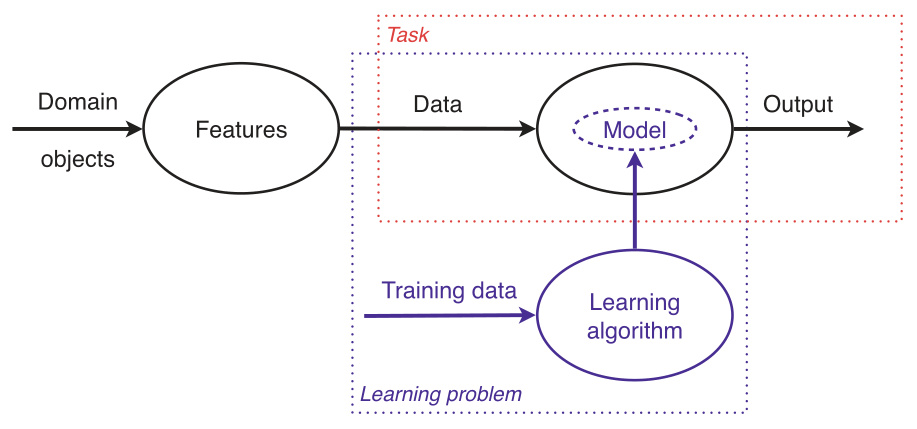
\includegraphics[width = 0.8\textwidth]{./Figures/machine_learning_peter_flach.jpg}
\rule{35em}{0.5pt}
\caption[Machine Learning]{Machine Learning is used to perform complex tasks. A task will require a mapping - a model - of inputs to outputs. The creation of the mapping by using sample data the model will encounter is a machine learning problem. }
\label{fig:machine_learning}
\end{figure}

%Kinds of Machine Learning
Machine Learning comes in three main categories; \textit{Supervised}, \textit{Unsupervised} and \textit{Reinforcement Learning}.
%Supervised
In Supervised Learning the algorithm is provided with many examples of input and the desired output for training.
To be more precise, given a set of data $D = ((\vo{x^n}, y^n), n = 1, ..., N )$, the algorithm must learn the relationship between the input vector $\vo{x}$ and the output $y$.
$\vo{x}$ is a vector of $m$ values, $\vo{x} = (x_1, x_2, ..., x_m)$ and $y$ is the corresponding output\citep{domingos2012few}.
A trained model can then take new input $\vo{x^\star }$ and predict the correct output $y^\star$.
We measure the degree of predictive success with the \textit{cost function}, $C(y^{pred}, y^{true})$, which takes the predictions and correct output as parameters.
Training the model is done by minimizing the cost function with respect to the model parameters.

%Supervised: Regression 
Supervised Learning itself has two sub-types - \textit{Regression} and \textit{Classification}.
Regression problems are concerned with giving real-valued output as a function of the input\citep{sammut2011encyclopedia}, see Figure ~\ref{fig:regression}.
There are many applications requiring numerical predictions on a continuum such as stock prices, temperatures and power generation.
\begin{figure}[htbp]
	\centering
		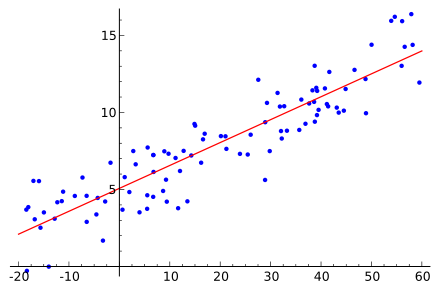
\includegraphics[width = 0.8\textwidth]{./Figures/regression.png}
		\rule{35em}{0.5pt}
	\caption[Regression]{In Regression a continuous output as a function of the features is learned. Here the examples (blue dots) have an output shown on the $y-axis $ as a function of a single feature, corresponding to the $x$-axis. While the examples clearly have the unmistakable pattern of an ascending straight line the regression model must be confused by the noise. The fitted model (shown in red) can be used to make predictions, $y_{pred} $, for the output of a new example input, $x^\star $, that is close to the true output of $y^\star $.}
		\label{fig:regression}
\end{figure}

%Supervised: Classification
Classification is predicting classes having learned from examples.
For example, a bank may wish to classify loan applicants into `high-risk' and `low-risk' groups.
Unlike regression, the output $y$ can only take on the discrete values of `high-risk' or `low-risk'.
A model is built from the customers' historical data of income, savings, professions, ages and debt histories that can predict the risk class of a new applicant.
These items of information about the applicant are known as \textit{features}.
If we look into the \textit{feature space}, a space made with each feature as a spacial dimension, we can create a model that separates the two classes, see Figure ~\ref{fig:classification}.
Features relevant to an applicant's financial capacity can provide many weak relations associated with their loan risk\citep{alpaydin2004introduction}.

This resulting model can also be analysed to reveal the data's underlying structure.
In the bank example, researchers can find common attributes of low-risk customers useful for target advertising for new and safe loans.
\begin{figure}[htbp]
	\centering
		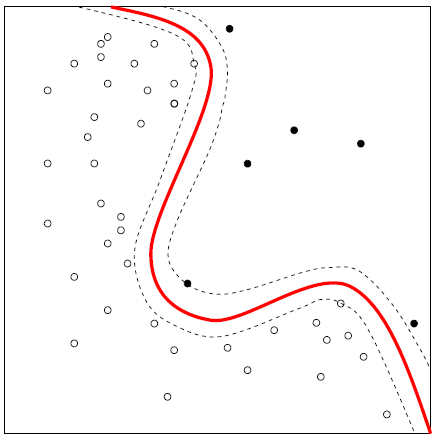
\includegraphics[width = 0.4\textwidth]{./Figures/classification.png}
		\rule{35em}{0.5pt}
	\caption[Classification]{Two different classes (circles and dots) fill the two dimensional feature space. Classification is the building of a model that can separate the classes such that for any new feature vector, $x^\star$, the correct class can be predicted. The model shown by the red line cuts across the feature space to differentiate the class of objects on one side versus the other.
	This algorithm used here tries to produce a boundary that is equally distant between the nearest examples, as shown by the broken lines to either side of the border. If a new object which lies to the top-right of the feature plane were discovered the model can be used to predict that it should be a dot. }
		\label{fig:classification}
\end{figure}

A regression model can tackle classification problems by assigning a level of confidence for an object belonging to a class.
This is often done by giving a prediction between zero and one.
The continuous output is then discretized, often by thresholding, to get a discrete label.
For example, output above 0.5 would be classified as a cat and below 0.5 as a dog.
Multi-label problems however cannot be answered by a single-valued output.
A classic example used within machine learning texts\citep{lecun2007mnist} is that of optical character recognition; recognizing printed or written numeric characters from their scanned images.
Such multi-label problems are treated by producing an output vector, $\vo{y}$, of ten values between zero and one.
Should the second value in the vector be the largest this would mean the digit is classified as a two.
The vector $\vo{y}_i = (0, 1, 0, 0 , 0, 0, 0, 0, 0, 0)$ would symbolise the label as being a two as the $1$ is in the second position.
Similarly $\vo{y}_i = (0, 0, 1, 0, 0, 0, 0, 0, 0, 0)$ represents a three.
This method of numerically encoding discrete labels is known as \textit{one-hot encoding}.

%Unsupervised Learning
Ideally machines would learn about the world as babies in that they learn to distinguish objects and people without being given explicit labels.
Machine Learning could then be much more useful as there is far less labelled data.
Learning models without data labels is known as \textit{Unsupervised Learning}.
Unsupervised algorithms attempt to find an accurate but compact description of the data\citep{barber2012bayesian}.
Once built, the model can be used to find clusters, as in Figure ~\ref{fig:Clustering}, compress the data or generate more with the same structure.
%[show this twice, once without colour] 
\begin{figure}[htbp]
	\centering
		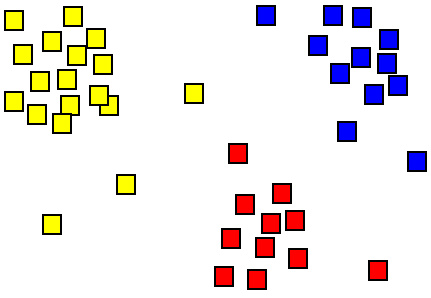
\includegraphics[width = 0.5\textwidth]{./Figures/clustering.jpg}
		\rule{35em}{0.5pt}
	\caption[Clustering]{While data may not have labels, Unsupervised Learning may still be used to uncover some inherent structure. Here indistinguishable objects, shown as squares, are in the two dimensional feature space. A common Unsupervised Learning method of \textit{Clustering} may be used to uncover how many clusters there are within the data and where in the feature space they lie.}
		\label{fig:Clustering}
\end{figure}

Semi-supervised learning is the common scenario in which there is little labelled but plenty unlabelled data.
For example, there are many millions of images of trees on the internet, but few of the images will specify the species.
Pure Supervised Learning would be forced to use only the labelled images and cast away the rest, losing valuable information.
Semi-supervised learning takes a more advanced approach and uses the unlabelled data to enhance the learning process.
The unlabelled data is used to `prime' the model, narrowing in on a range of useful parameter initializations before supervised learning begins.
The \textit{pre-training} makes the model come to recognize trees, even though it cannot yet distinguish species.
It will come to expect trunks, branches, green leaves and bark.
From there, the subtleties of variations that distinguish species can then be taught using the limited labelled data.
The final model will generally be better than one trained on the labelled data alone as shown in Figure ~\ref{fig:Unsupervised_learning}.
\begin{figure}[htbp]
	\centering
		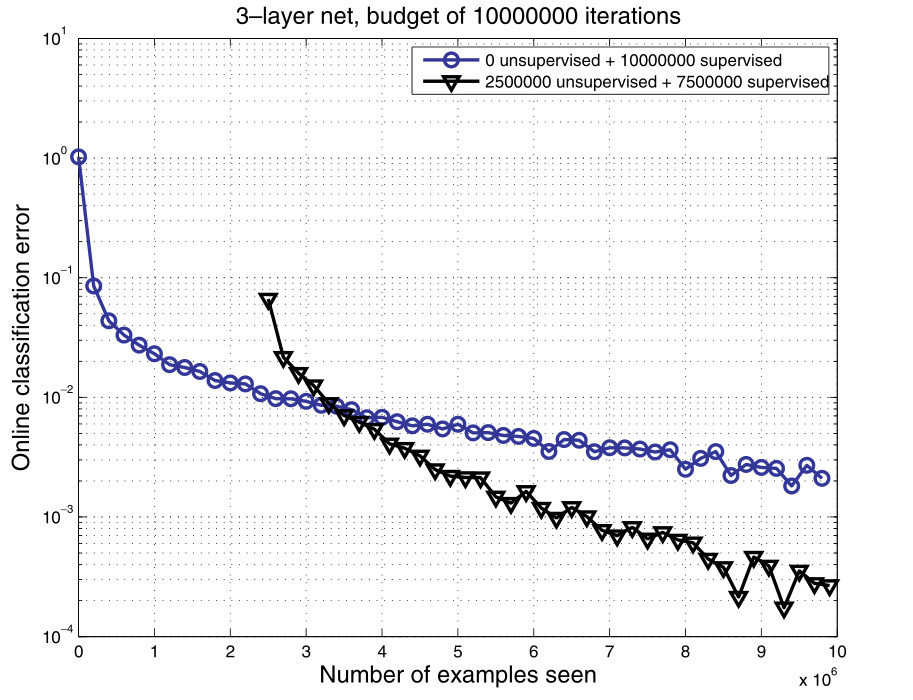
\includegraphics[width = 0.8\textwidth]{./Figures/Learning_deep_architectures_for_AI_Bengio_unsupervised_learning.jpg}
		\rule{35em}{0.5pt}
	\caption[Semi-supervised Learning]{A semi-supervised model (shown in black) was shown 2.5 million examples without labels. These were used to instantiate the model parameters with better starting values than randomness would have produced. In this case, the semi-supervised model outperforms the supervised model (shown in blue), with parameters settled on sub-optimal values due to the worse initialised parameter values. Analogously it is much easier to teach someone to recognize different bird species (the labels) when they are accustomed to what birds generally look like. The oscillations to the far right of the semi-supervised model result from the error being so close to zero that sampling variations appear large on the log-scale.}
	\label{fig:Unsupervised_learning}
\end{figure}

Instead of predicting output or uncovering structure, \textit{Reinforcement Learning} handles an agent in an environment, like a character in a game world.
The object is to maximize the agent's behaviour - its actions in response to its environment - when a reward is received over time or only at the very end.
Figure ~\ref{fig:Reinforcement _Learning_2} shows an AI system that can learn to play Atari games without explicit instructions at all.
Unlike Supervised Learning the agent is not informed of correct and incorrect behaviours but unlike Unsupervised Learning there is some feedback on performance.
If the game character's reward is its survival time it must learn life-span enhancing behaviour, such as eating, and avoiding dangerous actions, like drinking poison.
\citep{barber2012bayesian}

\begin{figure}[htbp]
	\centering
		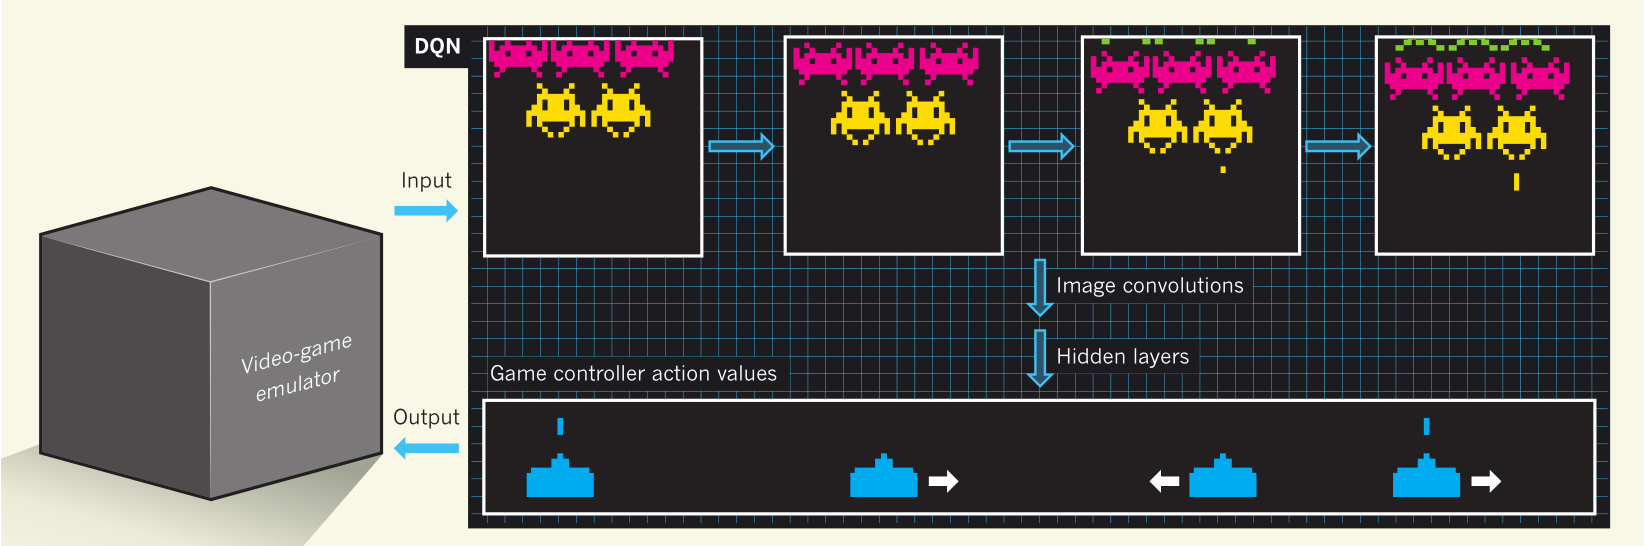
\includegraphics[width = 1.0\textwidth]{./Figures/Reinforcement_Learning_Learning_to_see_and_act.jpg}
		\rule{35em}{0.5pt}
	\caption[Reinforcement Learning]{The `Deep Q-Network' analyses four sequential video frames and predicts future game score for each possible action. This system is not even given instructions as to what objects to avoid, the characteristic elements of the game or how each control will impact the score. Instead information is extracted from the pixels through image convolutions and hidden layers [described in Section ~\ref{sec:neural_networks}] and fed to the Reinforcement Learning algorithms which must learn to recognize game elements and their attributes and which actions in different game states most improve the score.}
	\label{fig:Reinforcement _Learning_2}
\end{figure}

Sometimes new information becomes available over time. 
This means the model would have to be entirely retrained on the expanded data-set, a time-consuming task. 
\textit{On-line learning} is used to combat this problem.
Predictions are made on each instance in a series and it will receive a reward or loss after each one\citep{sammut2011encyclopedia}.
It is not necessarily supervised or unsupervised as incoming data may or may not have labels.
The model's objective is to maximise accumulated reward (or minimize the accumulated loss).
Expressed formally:
For each item in the sequence $s = 1, 2, 3, ...$, the algorithm:
\begin{enumerate}
\item Takes input $x_s \in X$
\item Makes prediction $y_s \in Y$
\item Receives a response $z_s \in Z$
\item Incurs a cost $c_s = c(y_s, z_t)$
\end{enumerate}
On-line learning is similar to reinforcement learning however the reward is instantaneous.

\subsection{Features}
%Features:Binary/Nominal/Continuous
In all machine learning applications features come in three types.
\textit{Binary Features} can take on only True or False values (numerically represented as $1$ and $0$).
For instance a feature `being human' can only be true or false.
\textit{Nominal Features} are multi-valued but discrete, such as a person's shoe size.
\textit{Real Features} can take on a continuous range of values such as someone's height.

%Features:correlated redundant irrelevant 
Not all features are equally useful for a machine leaning practitioner.
Some features are irrelevant and only serve to add noise to the data-set which can decrease performance.
A person's favourite colour would likely not help predict their income.
Correlated features are ones that are related to each other.
For example a person's weight is strongly correlated with their height.
As a person's height increases, their weight usually does too.
Including their weight to the feature-set would add information but not as much as an uncorrelated (but relevant) feature would.
Lastly, a feature may be entirely redundant (a correlation coefficient of 1 or -1) adding no new information that is not already captured in the data.
For example, a copied column of useful features would be relevant but redundant. 

\section{Neural Networks}\label{sec:neural_networks}
%Introduction
%History Outline
%The perceptron (natural comparison)
%Activation Function
%Networking Perceptrons
%MLPs

%Introduction
\textit{Artificial Neural Networks} (ANNs) are one of many Machine Learning algorithms used.
In Deep Learning applications, which we shall cover in Section ~\ref{sec:deep_learning}, ANNs are almost exclusively used.
For us they will make an indispensable start toward Deep Learning techniques and serve as a platform for more in-depth ML understanding.
A simple definition of an ANN was provided by an influential figure in neuro-computing, Dr. Robert Hecht-Nielson.
He defines a neural network as ``\textit{...a computing system made up of a number of simple, highly interconnected processing elements, which process information by their dynamic state response to external inputs}"\citep{caudill1989neural}.
ANNs derive their name from being simplistic models of biological neural networks found within brains, see Figure ~\ref{fig:Biological_Neuron} 
\begin{figure}[htbp]
	\centering
		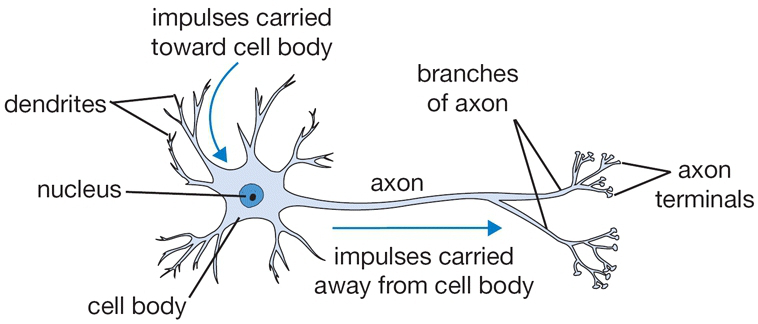
\includegraphics[width = 0.7\textwidth]{./Figures/neuron.png}
		\rule{35em}{0.5pt}
	\caption[Biological Neuron]{ANNs are loosely inspired by the structure and operation of biological neurons. The neuron receives information in the form of of potential differences at the tips of the dendrites. These electrical impulses are then carried toward the cell body which will itself emit an electrical signal along the axon to other neurons. The emission of an electric spike is dependent on the information received at the dendrites and the `chemical computation' of those inputs within the cell. Biological neurons either fire or they do not, but do not emit a continuous range of potential differences as an artificial neuron does.}
	\label{fig:Biological_Neuron}
\end{figure}

%History Outline
The first neural network model was developed with electrical circuits by Warren McCulloch and Walter Pitts in 1943\citep{mcculloch1943logical}.
However the model lacked a mechanism for learning.
Since then there have been many improvements\citep{bengio2009advances}.
The advent of significantly faster computers in the 50's allowed for larger networks\citep{bengio2009advances} leading IBM to form a research group to study pattern recognition and information theory under the leadership of Nathaniel Rochester\citep{bengio2009advances}.
They developed and simulated abstract neural networks on the new IBM 704 computer.
By 1959 neural network models called ``ADALINE" and ``MADELINE'' were designed that were similar to the ANNs of today\citep{bengio2009advances}.
MADELINE was more advanced than her counterpart and was the first ANN applied to solve a real problem; eliminating echoes on phone lines.
Then in 1962 a significant step was made; a learning algorithm, the Windrow-Hoff rule, was developed that could change parameter values as a function of the prediction error\citep{bengio2009advances} making the neuron perform better.

Despite the promising success with neural networks, interest faded in favour of Von Neumann computing architecture in a period known as the \textit{AI winter}\citep{kurzweil2014singularity}. 
This was partly the result of the early successes which led to over-expectations for what neural networks are capable of.
The inevitable disappointment led to research and funding being drastically decreased.

In 1986 three independent research groups tackled a method to extend the Windrow-Hoff rule to multi-layer networks and came up with similar ideas regarding the what is now called \textit{back-propagation} 
The development of this powerful training algorithm combined with faster computers thawed neural networks out of obscurity.

%The perceptron (natural comparison)
No understanding of neurons would be complete without first understanding \textit{Perceptrons}\citep{mo2012survey}.
Developed in the 50's and 60's by Frank Rosenblatt, a perceptron consists of one or more inputs, a processor and a single output\citep{mo2012survey} illustrated in in Figure ~\ref{fig:Perceptron}.
The flow of information follows a ``feed-forward model".
This means $m$ inputs, represented by the real-valued $\vo{x} = (x_1, x_2, x_3, ... , x_m)$, are fed to the perceptron which computes a single result.
Each input value, $x_i$, is multiplied by a corresponding real-valued \textit{weight} $w_i$ when grouped forming a real-valued weightings vector $\vo{w} = (w_1, w_2, w_3, ..., w_m)$.
All weighted inputs are summed, which can be represented as a dot-product
\be
\sum^m_{i = 1} x_i w_i = \vo{x} \cdot \vo{w}
\ee
where $m$ is the number of inputs.
Should the sum be greater than the threshold $0$, the perceptron outputs a $1$, otherwise a $0$.
Expressed as a function this reads,
\be
    f(\vo{x}) = 
\begin{cases}
   	1	,		& \text{if } \vo{x} \cdot \vo{w}\geq 0\\
    0	,     	& \text{otherwise}
\end{cases}
\ee
The larger the absolute value of a weighting $|w_i|$ the more the corresponding input $x_i$ contributes to the sum.
A positive weighting increases the likelihood of `exciting' the neuron which leads to an output of $1$.
Negative weights will reduce the sum and so `inhibit' the neuron.
Weightings can be tuned so the neuron is more responsive to specific inputs, some of which will be excitatory and others inhibitory.
Similarly changing the threshold affects the output but in the reverse manner to the weightings.
\textit{Decreasing} the threshold increases the likelihood of the neuron `firing' whereas increasing the threshold decreases the likelihood.
Threshold varying is equivalent to holding the threshold constant and adding a \textit{bias}, a constant $b$, to the dot-product.
\be
    f(\vo{x}) = 
\begin{cases}
   	1	,		& \text{if} \vo{x} \cdot \vo{w} + b \geq 0\\
    0	,     	& \text{otherwise}
\end{cases}
\ee
A positive bias is then excitatory, and negative is inhibitory.
This still is not optimal as now weightings and an additional bias term must be tuned.
Instead the bias is absorbed into the dot-product by introducing an extra input of $x_0$ which is always equal to one with its corresponding weighting of $w_0$.
By varying the weighing $w_0$ this is equivalent to changing the value of the bias term.
Now all neuron tuning is done on the weightings.

%Activation Function
Till now we made the neuron output only a zero or one according to a threshold.
There is no reason why the output cannot be some other function $f(\vo{x} \cdot \vo{w})$, known as the \textit{activation function}.
Many different activation functions have been used throughout ANN's development.
The function favoured today is the Rectified Linear Unit (ReLU) or $max(0, X)$.
ReLU activations will grow linearly for $X > 0$ but are $0$ where $X < 0$.
Research has shown they make training quicker and have better overall results\citep{NIPS2012_4824}.

%Networking Perceptrons
A perceptron can learn a limited number of relations between inputs\citep{mo2012survey}.
In particular the exclusive-or (XOR) function is beyond its learning capability as shown in 1969 by Marvin Minsky and Seymour Papert\citep{minsky1969perceptrons}.
However the output of one neuron may fed as the input to another neuron and so on forming a network.
Combining many simple elements into a network can produce a much more complex system\citep{bar1997dynamics}.
Networks differ in kind but all share the same components: \textit{nodes}, and connections between them\citep{gershenson2003artificial}.
Individual nodes can be thought of as computational units or neurons.
Each receives input and processes the information to generate an output.
The processing may be very basic (such as a simple summation of the input) or more complex.
Connections between the nodes determine the direction of information flow.
Interactions between the nodes lead to the complex emergent behaviour of the network.
\begin{figure}[htbp]
	\centering
		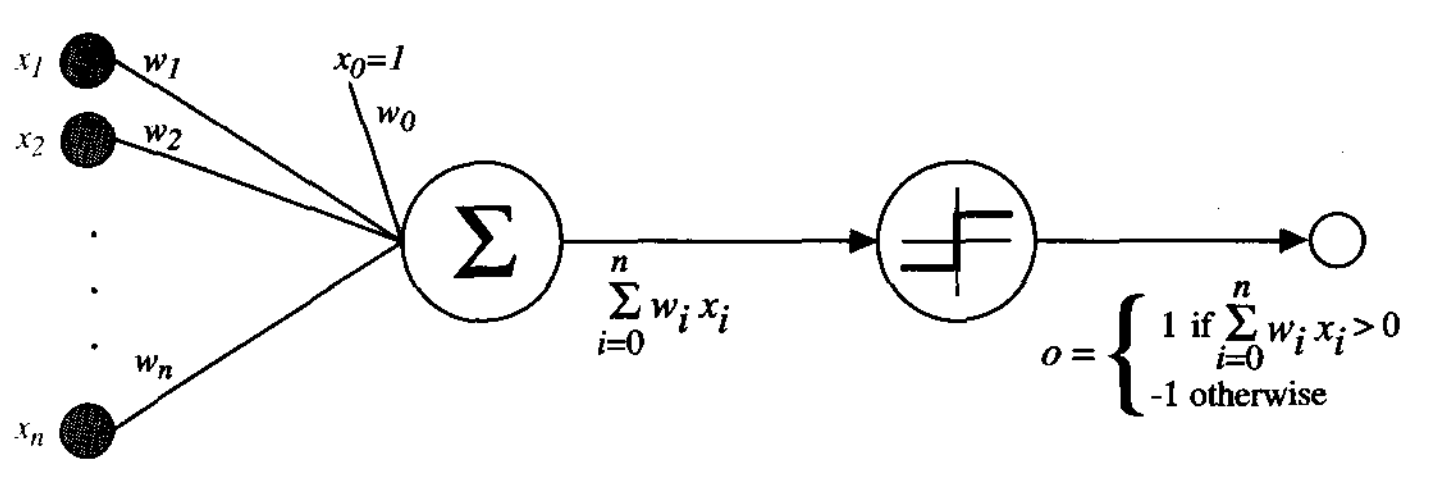
\includegraphics[width = 1.0\textwidth]{./Figures/ML_tom_mitchel_perceptron.PNG}
		\rule{35em}{0.5pt}
	\caption[The Perceptron]{A Perceptron is a simple model of a neuron. Input is given in the form of a linear weighted sum, $\sum^n_{i = 0} w_i x_i$, over all $n$ input values. The result is used as input for the (often non-linear) \textit{activation function}. For the first perceptrons this was the step-wise function which outputs $1$ if the sum is greater than $0$, otherwise a $-1$}
	\label{fig:Perceptron}
\end{figure}

%MLPs
\begin{figure}[htbp]
	\centering
		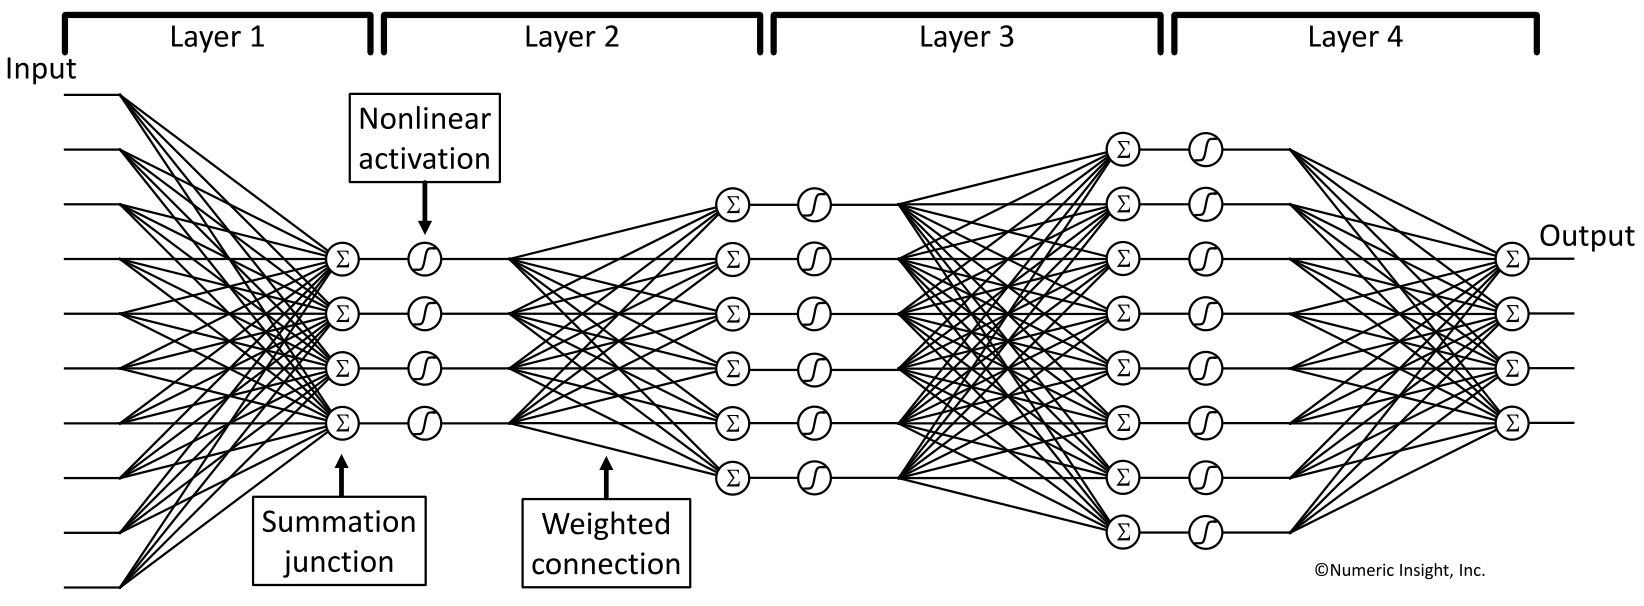
\includegraphics[width = 1.0\textwidth]{./Figures/MLP_a_survey_time_travel_in_DL_4.jpg}
		\rule{35em}{0.5pt}
	\caption[Multi-Layer Perceptron]{Pictured above is the architecture of a Multi-Layer Perceptron (MLP). An MLP is an example of a `feed-forward' network as information flows through the network in one direction only (left to right in the figure). The network is composed of an arbitrary number of layers but will always have an \textit{input layer} (on the far left) which receives the features and an \textit{output layer} (on the far right) which returns the model results. Each perceptron within Layer 1 takes a weighted sum - connection weightings can differ between neurons - of the input features through a non-linearity (often a sigmoidal function). The singular output of each input node forms one feature for the next layer to the right, the first \textit{hidden layer}. Similarly output from each of the Layer 2 neurons serves as input features to Layer 3, the second hidden layer. Finally layer 4, the \textit{output layer}, computes the model result. As there are four output nodes, this MLP provides four different answers. For example each of the four neurons may give output representing the model's confidence that the input example image features belong to a cat, dog, man or mouse respectively. The Layer 4 neuron with the largest output will then determine to which of the classes the item belongs. }
	\label{fig:MLP}
\end{figure}
Feed-forward ANNs, are organized into layers.
There are at least two layers to a neural network such as in Figure ~\ref{fig:MLP}; the first layer, or \textit{input layer}, and the last layer, the \textit{output layer}.
Should there be layers between, they are known as \textit{hidden layers}.
The output from all input layer neurons are fed as input to second layer neurons.
The second layer's output is now based on the results from the input layer.
A feed-forward system allows proceeding layers make decisions at a more abstract level than preceding layers\citep{krose1993introduction}.
These networks are much more capable of fitting to arbitrary feature relations.
In fact they can compute any continuous function\citep{hornik1989multilayer}.
Changing one neuron to act as an AND logic gate is easily done by hand.
However for ANNs that have hundreds or thousands of neurons an algorithm must be used to train the weightings.

\subsection{Training}
%backpropogation
	%Last Layer
	%Hidden Layers
%SGD
%Momentum, Adagrad etc..
%Learning Decay
%Activation Fucntions
%Weight Initialization
%Batch Norm
%Final layer norm
%GPU acceleration

%Regularization
	%Dropout
	%Early Stopping

Geoffrey Hinton, around 1985, developed a multi-layer neural network that could learn more functions than the single layer perceptron could\citep{mo2012survey}\citep{williams1986learning}.
Hinton also developed the training algorithm for multi-layered neural networks called \textit{back-propagation}\cite{mcclelland1986parallel}.
Back-propagation is a supervised learning training method whereby the cost is calculated.
The cost is a measure of the difference between output nodes of the network and their target values.

Mean Squared Error (MSE) is a common cost function used in regression models.
It is just the difference between the true value of example $i$, $y_i$, and the predicted value, $y_i^\star$.
\be
MSE = \frac{\sum^n_{i = 1}(y_i - y_i^\star)^2}{n} 
\ee
where $n$ is the number of examples in the test set, $y_i$ is the true label for example $i$, and $y_i^\star$ is the predicted value,

Back-propagation is aptly named as the cost is propagated backward though the network, adjusting connection weightings, or moving to a different location in `weight space' to reduce the error at every stage.
%\begin{figure}[htbp]
%	\centering
%		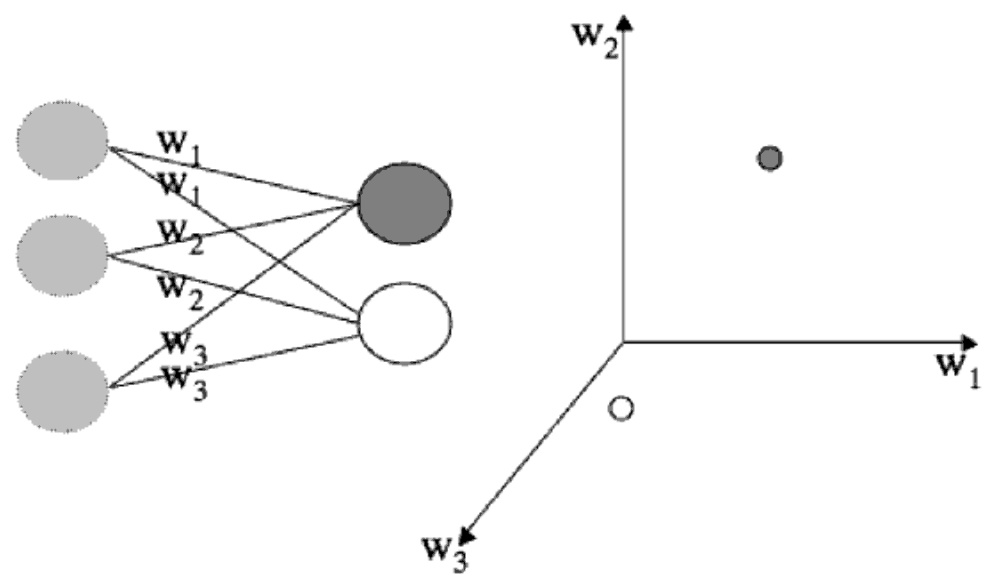
\includegraphics[width = 0.5\textwidth]{./Figures/machine_learning_an_aglorithmic_perspective_weight_space.jpg}
%		\rule{35em}{0.5pt}
%	\caption[Weight Space]{All the parameters in a model can be thought of as dimensions of `Weight Space'. All weightings of a neural network are represented by a single point in weight space. The objective of model training is to move this point in weight space from where it is currently located (in gray) to one in which the network makes better predictions (outlined).}
%	\label{fig:Weight_space}
%\end{figure}
\begin{figure}[htbp]
	\centering
		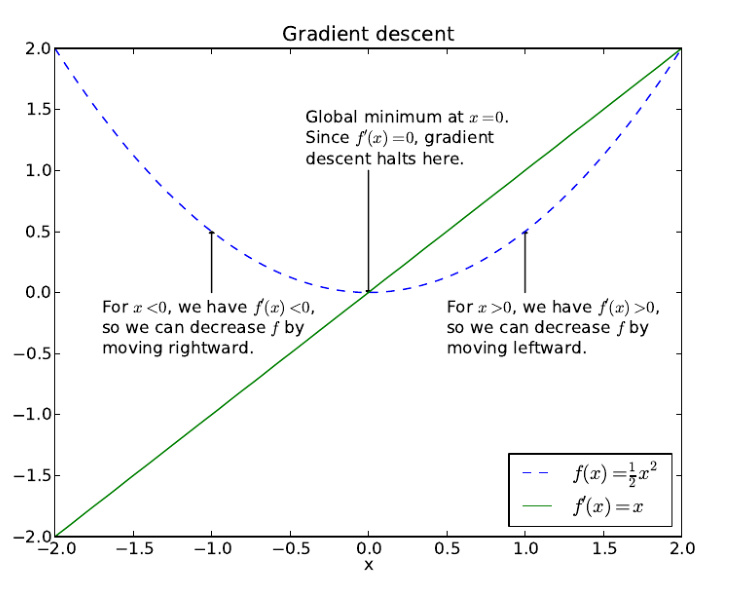
\includegraphics[width = 0.8\textwidth]{./Figures/gradient_descent_DL_textbook_8.jpg}
		\rule{35em}{0.5pt}
	\caption[Gradient Descent]{A neural network like many machine learning models can be highly complex, non-linear and non-convex. 
A function, $f(x)$, is convex over an interval $[a, b]$ if the second derivative $f^{\prime \prime}(x) \geq  0$ for all $x$ in $[a, b]$.
It may not be possible to analytically calculate the optimal parameters for the model. However we can use gradient descent to slide down the surface of the cost function to a minima. Consider the simplified cost equation of $f(x) = \frac{1}{2}x^2$. Left of the minima at $x = 0$ the derivative, $f^\prime(x) = x$, will be negative. So we can decrease the value of $f(x)$ by choosing a new value for $x$ to the right of its previous position. Similarly where $x$ is positive the derivative will be positive and so moving leftward will bring us closer to the minima.}
	\label{fig:Gradient_descent}
\end{figure}
\begin{figure}[htbp]
	\centering
		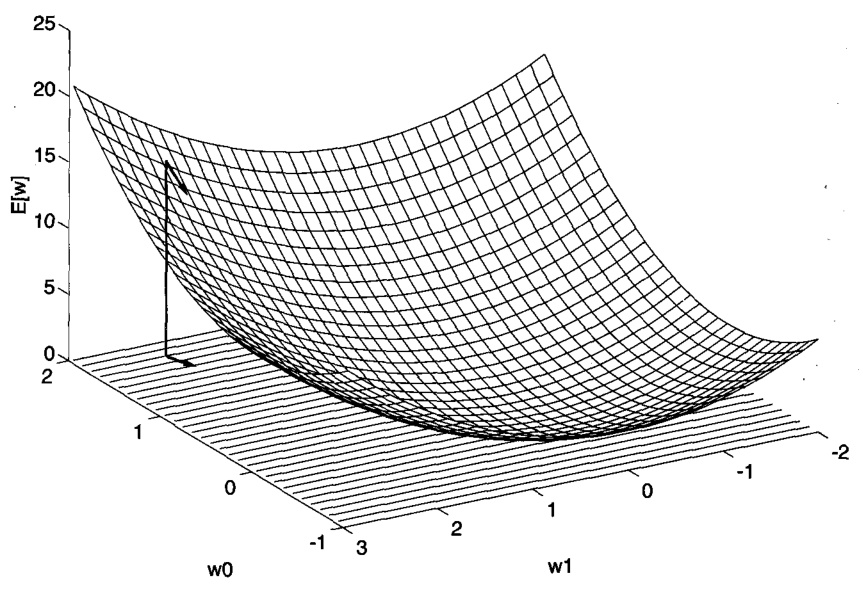
\includegraphics[width = 0.6\textwidth]{./Figures/ML_tom_mitchel_gradient_decent.jpg}
		\rule{35em}{0.5pt}
	\caption[Multi-dimentsional gradient descent]{Where the cost function is a surface in a multidimentsional space, here $w0$ and $w1$, the negative of the derivative at any point will point in the direction of steepest decent. Updating the weights to new values close to the last position but in the direction of steepest descent will reduce the cost of the model.}
	\label{fig:Gradient_descent_2}
\end{figure}

\textit{Gradient descent} is the method used to tune the weights once we have the cost.
The cost function can be pictured as a surface of height parametrised by the weightings, see Figure ~\ref{fig:Gradient_descent} for a detailed picture.
The cost-surface will have many peaks, local maxima, and troughs, local minima.
Weights are usually initialized to take on random values; the exact distribution from which they are sampled can vary.
All the weight co-ordinates will specify a point in the cost-landscape.
The lowest possible cost, and so the best fit of the neural network, lies in the deepest trough, the global minima.
Gradient descent looks at the immediate area around the current location, see Figure ~\ref{fig:Gradient_descent_2}, and walk down the path of steepest descent.
As gradient descent only walks downhill, and not up, there is no guarantee that it will reach the global minima.
Gradient descent cannot climb a peak to get to a deeper trough.
Finding the gradient of a function is in principle straight forward but can get messy.
First lets define some notation referring to Figure ~\ref{fig:MLP_2}:
$z_j$ is the weighted input sum of node $j$ in layer $l$.
$g_j$ is the activation function applied to $z_j$ at node $j$ in layer $l$.
$a_j$ is the activation, the output of $a_j = g_j (z_j)$ at node $j$ in layer $l$.
$w_{ij}$ is the weight connecting node $i$ in layer $(l-1)$ to node $j$ in layer $l$.
$t_k$ is the target prediction for the $k$'th neuron in the output layer.

\begin{figure}[htbp]
	\centering
		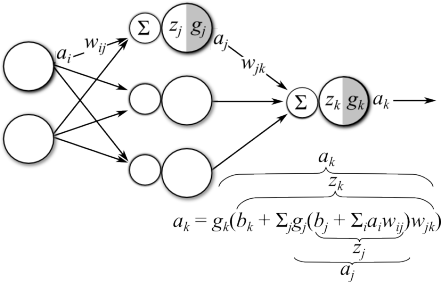
\includegraphics[width = 0.7\textwidth]{./Figures/neural_net.png}
		\rule{35em}{0.5pt}
	\caption[MLP Notation]{The effective algebraic function of an MLP takes the form of activation functions nested inside each other. Input activation values, or features, $a_i$ are used in the weighted summation, $z_j = b_j + \sum_i a_i w_{ij}$, as part of the input to the next activation function, $g_j$, which determines the activation, $a_j = g_j(z_j)$. These values are in turn used in the weighted sum, $z_k = b_k + \sum_j a_j w_jk$ as input to the final activation function, $g_k$, to produce the activation of $a_k$. If the model parameters are tuned correctly $a_k$ should be close to the true output, $t_k$, corresponding to input features $a_i$. The training method of back-propagation uses the chain-rule of calculus to see what the effect a slight change to each parameter would make to the final result. The model will then update each parameter in the direction that to first-order brings the output closer to the true value\citep{backpropagationImage}.}
	\label{fig:MLP_2}
\end{figure}

%Last Layer
To take you through the back-propagation algorithm we will consider a \textit{Multi-Layer Perceptron} (MLP) with one hidden layer.
The first case we will look at is the weights connecting the final hidden layer to the output layer.
Nodes in the hidden layer are indexed by $j$, where there are $J$ nodes in the final layer.
The $K$ output nodes are similarly indexed by $k$.
For the cost function we will the squared difference between target values and the network predictions.
This is often used in regression problems, here we use it for simplicity.
The cost function $C$ is therefore
\be
C = \frac{1}{2}\sum_{k\epsilon K} (a_k - t_k)^2
\ee
A factor of $\frac{1}{2}$ does not affect the results and is used for later convenience.
The function returns the cost of a single feed-forward prediction relating to a single example's features.
The total cost is the sum of every individual prediction's cost.
This is because we do not wish to make the network very good at recognizing only one item, but instead predict very well on the whole data set.

We can use the chain rule to calculate the gradient of the cost with respect to each weight, $w_{ij}$.
\be
\begin{aligned} \label{eq:cost_derivitive}
\frac{\partial C}{\partial w_{jk}} 	&= \frac{\partial}{\partial w_{jk}} \left(\frac{1}{2} \sum_{k\epsilon K} (a_k -t_k)^2\right)\\
									&= (a_k-t_k)\frac{\partial}{\partial w_{jk}} (a_k -t_k)\\
\end{aligned}
\ee
We drop the summation as only one term survives the differentiation.
The weight $w_{jk}$ connects the $j'th$ neuron in layer $l-1$ to only the $k$th output node therefore every other output node has no dependence on $w_{jk}$ and so all other derivatives are zero.
Looking at the partial derivative in Equation ~\ref{eq:cost_derivitive} we get
\be
\frac{\partial C}{\partial w_{jk}} = (a_k-t_k)\frac{\partial}{\partial w_{jk}} (a_k)
\ee
since $t_k$ is independent of the weights.
Now we use the chain rule again on the activation $a_k = g_k (z_k)$
\be
\begin{aligned} \label{eq:z_d_w}
&= (a_k-t_k)\frac{\partial}{\partial w_{jk}} [g_k (z_k)]\\
&= (a_k-t_k) g_k^\prime (z_k) \frac{\partial}{\partial w_{jk}} z_k
\end{aligned}
\ee
The weighted sum in the output layer is given by $z_k = \sum_{j\epsilon J} g_j (z_j)w_{jk}$.
Taking the partial derivative we get $\frac{\partial z_k}{\partial w_{jk}} = g_j (z_j) = a_j $.
Again only one term survives from the summation, but this time of index $j$.
Substituting this simple result in place of $\frac{\partial z_k}{\partial w_{jk}}$ in Equation ~\ref{eq:z_d_w} we have 
\be
\frac{\partial C}{\partial w_{jk}} = (a_k-t_k) g_k^\prime (z_k)a_j
\ee
where $g_k^\prime$ is shorthand for $\frac{\partial g_k(z_k)}{\partial w_{ij}}$.
We see the derivative is a product of three terms:
The difference between prediction and target value of neuron $k$; second is the derivative of node $k$'s activation function from the last layer; lastly is the activation of node $j$ in the previous layer.
Grouping all terms involving $k$ under $\delta_k$ we get
\be
\frac{\partial C}{\partial w_{jk}} = \delta_k a_j
\ee
where
\be
\delta_k = (a_k-t_k) g_k^\prime (z_k)
\ee
The $\delta_k$ can be thought of as a measure of the error at $t_k$.
The error is back propagated to all the weights $w_{1k}, w_{2k}, w_{3k}, ... , w_{Jk}$ in proportion to activation values $a_1, a_2, a_3, ... , a_J$.
In doing this we find each weight's contribution toward the error we wish to minimize.
So we now update the weights as $w_{jk}\leftarrow w_{jk} - \eta \frac{C}{w_{jk}}$ where $\eta$ is the magnitude of the step, or the \textit{step size}.
For all $N$ examples within the data-set we sum the $N$ steps $\eta \frac{C}{w_{jk}} $ so as to average the best possible step to minimize the total cost.
Too small a step size means the algorithm will take too long to converge, and perhaps get stuck in local minima.
Too large a step size and gradient descent can overshoot minima altogether, or oscillate over the minima never settling in the local minima, see Figure ~\ref{fig:global_and_local_minima} for better understanding.
\begin{figure}[htbp]
	\centering
		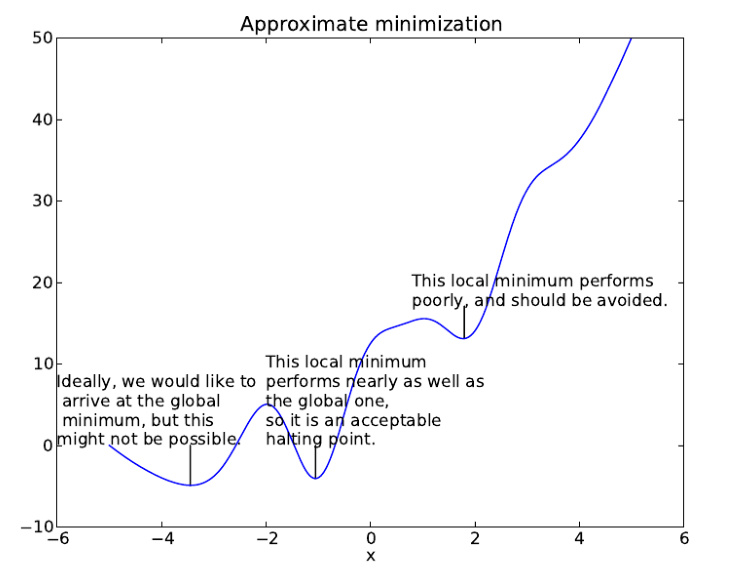
\includegraphics[width = 0.9\textwidth]{./Figures/global_verse_local_minimum_DL_textbook_9.jpg}
		\rule{35em}{0.5pt}
	\caption[Local Minima]{Navigating the cost function is not as simple as the case in Figure ~\ref{fig:Gradient_descent_2}. The surface will likely not have one local minima but many. Training the network by sliding down the cost surface can trap the model in a sub-optimal local-minima. The ideal is to find the global minima as in the image above, however this may be too hard to find. Therefore many local-minima which perform nearly as well as the global minima are acceptable halting points for training.}
	\label{fig:global_and_local_minima}
\end{figure}
%Middle Layer
We now proceed with how to update the weights for all layers other than the last hidden one.
Now $i$ indexes nodes in layer $(l-1)$ and $j$ those of layer $l$.
The derivative with respect to inner layer weights is
\be
\begin{aligned} \label{eq:dC_dw}
\frac{\partial C}{\partial w_{ij}} 	&= \frac{\partial}{\partial w_{ij}}\frac{1}{2} \sum_{k\epsilon K} (a_k -t_k)^2\\
									&= \sum_{k\epsilon K}(a_k-t_k)\frac{\partial}{\partial w_{ij}} (a_k)
\end{aligned}
\ee
This time the sum is not dropped as every node in the hidden layer affects every node in the output layer.
Substituting $a_k = g_k (z_k)$ into Equation ~\ref{eq:dC_dw} we obtain
\be
\frac{\partial C}{\partial w_{ij}}	= \sum_{k\epsilon K}(a_k-t_k) \label{eq:derivitive_into} g_k^\prime(z_k)\frac{\partial}{\partial w_{ij}} (z_k)
\ee
Now 
\be
\begin{aligned} \label{eq:Z_kDecompose}
z_k &= \sum_{j\epsilon J} a_j w_{jk}\\
	&= \sum_{j\epsilon J} g_j (z_j)w_{jk}\\
	&= \sum_{j\epsilon J} g_j \left(\sum_{i\epsilon I} z_i w_{ij}\right)w_{jk}
\end{aligned}
\ee

After decomposing $z_k$ in Equation ~\ref{eq:Z_kDecompose} we determine $\frac{\partial z_k}{\partial w_{ij}}$ with the chain rule.
\be
\begin{aligned}
\frac{\partial z_k}{\partial w_{ij}} &= \frac{\partial z_k}{\partial a_j} \frac{\partial a_j}{\partial w_{ij}}\\
 & = \frac{\partial}{\partial a_j}(a_j w_{jk}) \frac{\partial a_{j}}{\partial w_{ij}}\\
 & = w_{jk} \frac{\partial a_j}{\partial w_{ij}}\\
 & = w_{jk} \frac{\partial g_j(z_j)} {\partial w_{ij}}\\
 & = w_{jk} g_j^\prime (z_j)\frac{\partial z_j }{\partial w_{ij}}\\
 & = w_{jk} g_j^\prime (z_j)\frac{\partial }{\partial w_{ij}}\left(\sum_{i\epsilon I} a_i w_{ij}\right)\\
 & = w_{jk} g_j^\prime (z_j) a_i
 \end{aligned}
\ee
plugging in this solution for $\frac{\partial z_k}{\partial w_{ij}} $ into Equation \ref{eq:derivitive_into} we have
\be
\begin{aligned}
\frac{\partial C}{\partial w_{ij}} &= \sum_{k\epsilon K}(a_k-t_k) g_k^\prime(z_k) w_{jk}g_j^\prime(z_j)a_i\\
&= a_i g_j^\prime(z_j) \sum_{k\epsilon K}(a_k-t_k) g_k^\prime(z_k) w_{jk}\\
&= a_i g_j^\prime(z_j) \sum_{k\epsilon K} \delta_k w_{jk}
\end{aligned}
\ee

Again we see errors back propagate with the error signal now being
\be
\delta_j = g_j^\prime (z_j) \sum_{k\epsilon K}\delta_k w_{jk}
\ee
such that

\be
\frac{\partial C}{\partial w_{ij}} = \delta_j a_i
\ee

To update the weights at layer $l-1$ the error signal of layer $l$ is back-propagated and weighted by the activation $a_i$.

What is particularly convenient about back-propagation is that all the operations are easily vectorizable.
There are many programming modules that perform vectorized equations significantly faster than iterating through all weights in a layer.
Graphics processing cards have thousands of cores which can do many thousands of algebraic equations at one.
We will come to the use of graphics cards later.

We can express this as a pseudo algorithm.

For each example $n$ in the training set of $N$ in total\citep{neuralnetworkswebsite}
\begin{enumerate}
\item Feed forward through each layer $l = 2, 3, .., L$ with
\be
z^{x,l} = w^l a^{x, l-1}
\ee
where 
\be
a^{x, l-1} = g(z^{x, l})
\ee
\item Compute the error at layer $L$:
\be
\delta^{x ,L} = \Delta_a C_x \odot g^\prime(z^{x, L})
\ee
where 
\be
\Delta_a C_x = \left[\frac{\partial C}{\partial a^L_1}, \frac{\partial C}{\partial a^L_2}, \frac{\partial C}{\partial a^L_3}, ..., \frac{\partial C}{\partial a^L_J}\right]
\ee
The element-wise product e.g.
$
\begin{bmatrix}
    2  \\
    3  \\
\end{bmatrix}
\odot
\begin{bmatrix}
    6  \\
   	7  \\
\end{bmatrix}
=
\begin{bmatrix}
    2\times 6  \\
    3\times 7  \\
\end{bmatrix}
$
is denoted by $\odot$.
\item Back-propagate through layers $l = (L, L-1, L-2, ..., 0)$ and
compute the error
\be
\delta^{x,L} = \left[(w^{l + 1})^T \delta^{x, l + 1}\right]\odot g^\prime(z^{x, l})
\ee
\item Update all weights according to Gradient Descent
for each layer update the weights according to
\be
w^l \leftarrow w^l - \frac{\eta}{N} \sum_{n\epsilon N} \delta^{n,l}(a^{n, l-1})^T
\ee
Each sweep through the entire data set is called an \textit{epoch}.
\end{enumerate}

\subsection{Advanced Training Methods}

%Weight Initializations
%SGD, Momentum, Adagrad, learning decay
Training an MLP with back-propagation as it was originally designed can take a long time.
Every training iteration requires several time-consuming stages even with vectorized computation.
Each training example must be fed-forward through the network.
Then each error must be back-propagated through the network.
Finally all the weights must be updated.
And that is just one iteration.
Back-propagation may not converge for thousands.

%Gradient Descent = Batch Gradient Descent
Standard gradient descent computes the gradient of the cost function, $C(\theta)$ , with respect to the parameters $\theta$ for the entire training set.
This is known as \textit{Batch Gradient Descent} and where weights are updated according to the following rule,
\be
\theta = \theta - \eta \dot \Delta_\theta C(\theta)
\ee
As the gradients need to be computed for the entire training set this can be a very slow training process and may be limited by memory size.
Such training is guaranteed to converge to the global minimum for convex surfaces such as in Figure ~\ref{fig:Gradient_descent_2}, and to a local minimum for non-convex surfaces.
%Stochastic gradient Descent
\textit{Stochastic Gradient Descent} (SGD) differs from batch gradient descent in that the model parameters are updated for each example $x^{(i)}$ and label $y^{(i)}$
\be
\theta = \theta - \eta \dot \Delta_\theta C(\theta; x^{(i)}; y^{(i)}) \label{eq:updateEquation}
\ee
Batch training may perform redundant calculations in large datasets where there are similar examples.
SGD however, performs a single update at a time and is much faster and can be used for on-line training.
On average the gradient will point in the correct direction with much less computation.

%Mini batch gradient decent
\textit{Mini-batch gradient descent} learns from both SGD and batch training and instead performs an update for every batch of $n$ training samples.
\be
\theta = \theta - \eta \dot \Delta_\theta C(\theta; x^{(i:i + n)}; y^{(i:i + n)})
\ee
In this way the high variance of parameter updates from SGD is reduced and training is faster\citep{lecun2012efficient}.
Common batch sizes vary between 2 to 256 examples.
Mini-batch training is what is commonly employed for training neural networks.
The term SGD is often used to describe mini-batch training.

The stochastic nature of the batch means the batch gradient will often differ from the complete set.
While that seems to be counter-productive the occasional mis-step means it is possible to step over local minima and find a deeper one.
Fewer samples increases the random mis-steps allowing much more exploration of the parameter-space.
However using too few samples has the side-effect of increasing the training time.
Every batch loaded contributes to the memory overhead.
SGD will spend a lot of time randomly jumping through the parameter space it will take a long time to converge.
However, the likelihood of finding a deeper minima is increased.

Too many samples within the batch will dampen the stochastic effect.
The more samples in a batch, the less time each epoch will take.
For best results the order in which the examples are fed to SGD in each epoch should be randomized\citep{lecun2012efficient}.

%Momentum
\textit{Momentum} is a method that helps SGD navigate surfaces which curve more steeply in one direction than in another, see Figure ~\ref{fig:Momentum_2}\citep{bengio2012practical}\citep{werbos1990backpropagation}.

This is done by smoothing out the SGD updates by adding a weighted average of prior gradients
\be
\mu = \gamma \mu_{t-1} - \eta.\Delta_\theta C(\theta)
\ee
\be
\theta = \theta - \mu_t
\ee

where $\gamma$, a hyper-parameter, is usually set to 0.9.
The momentum term increases the step-size for dimensions where gradients tend to point in the same direction and reduces step-size for dimensions where gradients often change directions.
The idea is that it removes some of the noise and oscillations SGD has, especially in the directions of high curvature, see Figure ~\ref{fig:Momentum_2} for an illustration.

Other extensions like Adagrad by Duchi\citep{duchi2011adaptive}, Nesterov accelerated GD\citep{nesterov1983method}, Adadelta by Zeiler\citep{zeiler2012adadelta} and Adam by Kingma and Ba\citep{kingma2014adam} are known to work equally well, if not better than standard momentum in certain cases.
\begin{figure}[htbp]
	\centering
		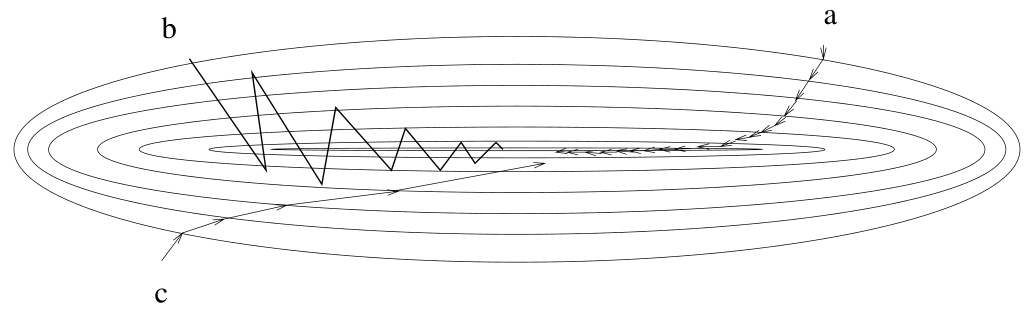
\includegraphics[width = 1.0\textwidth]{./Figures/momentum_An_introduction_to_NNs.jpg}
		\rule{35em}{0.5pt}
	\caption[Gradient Descent Comparisons]{The size of the step in weight space should be small enough so as to be in the region where the derivative is tangential to the surface, but too small and training may take a long time to converge, as in the case of path a. Too large a step-size will encourage the model to leap over the minima to the other side where the gradient has changed direction altogether. This leads to oscillatory behaviour, path b, where the model may never converge. Momentum, path c, starts with a small step-size, but increases the step size for the next iteration in the direction in which it last moved reaching the minima in much fewer steps.}
	\label{fig:Momentum_2}
\end{figure}

%Momentem Nesterov
Too much momentum will cause gradient descent to overshoot.
If the updates have a high momentum in one direction they will tend to overshoot the local minima repeatedly.
\textit{Nesterov Accelerated Gradient} tries to take into account the levelling off near the bottom in order to forcefully reduce the momentum.
If we use the momentum term $\gamma \mu_{t-1}$ to do the updates we can get an approximation for the next position by computing $\theta - \gamma_{t-1}$.
We can use this information to calculate the gradient not with respect to the \textit{current} parameters but with respect to the approximate future parameters:
\be
\mu_t = \gamma \mu_{t-1} - \eta \dot \Delta_\theta J(\theta-\gamma \mu_{t-1})
\ee
\be
\theta = \theta - \mu_t
\ee
where $\gamma$ will again be approximately 0.9.
%%adagrad
%\be
%g_{t,i} = \Delta_\theta J(\theta_i)
%\ee
%\be
%\theta_{t + 1,i} = \theta_{t,i} - \eta.g_{t,i}
%\ee
%\be
%\theta_{t + 1,i} = \theta_{t,i} -\frac{\eta}{\sqrt{G_{t, ii} + \epsilon}}.g_{t,i}
%\ee
%\be
%\theta_{t + 1} = \theta - \frac{\eta}{\sqrt{G_t + \epsilon}}\cdot g_t
%\ee
%%adadelta
%\be
%E[g^2]_t = \gamma E [g^2]_{t-1} + (1-\gamma)g_t^2
%\ee
%
%\be
%\Delta \theta_t = -\eta \dot g_{t,i}
%\ee
%
%\be
%\theta_{t + 1} = \theta_t + \Delta \theta_t
%\ee
%
%\be
%\Delta \theta_t = -\frac{\eta}{\sqrt{G_t + \epsilon}} \cdot g_t
%\ee
%
%\be
%\Delta \theta_t = -\frac{\eta}{\sqrt{E[g^2]_t + \epsilon}} g_t
%\ee
%
%\be
%\theta_t = -\frac{\eta}{RMS[g]_t}
%\ee
%
%\be
%E[\Delta \theta^2]_t = \gamma E [|delta \theta^2]_{t-1} + (1-\gamma) \Delta \theta^2_t
%\ee
%
%\be
%RMS[\Delta \theta]_t = \sqrt{E[\Delta \theta^2]_t + \epsilon}
%\ee
%
%\be
%\Delta \theta_t = -\frac{RMS[\Delta \theta]_{t-1}}{RMS[g]_t}g_t
%\ee
%
%
%\be
%\theta_{t + 1} = \theta_t + \Delta \theta_t
%%RMS prop
%\be
%E[g^2]_t = 0.9 E [g^2]_{t-1} + 0.1 g^2_t
%\ee
%\be
%\theta_{t + 1} = \theta_t - \frac{\eta}{\sqrt{E[g^2]_t + \epsilon}}g_t
%\ee
%%ADAM
%\be
%m_t = \Beta_q_m_{t-1} + (1-\Beta_1)g_t
%\ee
%\be
%\mu_t = \beta_2 \mu_{t-1} + (1-\beta_2)g^2_t
%\ee
%\be
%m^{^}_t = \frac{m_t}{1-\beta^t_1}
%\ee
%\be
%\mu^{^} = \frac{\mu_t}{1-\beta^t_1}
%\ee
%\be
%\theta = \theta - \eta.\Delt_\theta J(\theta)
%\ee
%
%\be
%\theta_{t + 1} = \theta_t - \frac{\eta}\sqrt{\mu^{^}_t} + \epsilon} m^{^}_t
%\ee

\section{Optimization}
	\subsection{Normalization}

In many machine learning problems some features will consistently have much larger values than others.
Consider the case of predicting house market value.
Two of the features may be the last sale price and the number of rooms.
Pricing may vary between R$500,000$ to R$20,000,000$, leaving a huge range in between, whereas the typical number of rooms varies over the small range of $1$ to $4$.
Some machine learning classifiers are immune to feature scaling, however gradient descent is negatively affected by features with values over different scales, making the process take longer\citep{featureScaling}.
For many algorithms, if there is a large discrepancy in the magnitude of features this can translate into the model overestimating the role of the larger magnitude feature.
Some algorithms for clustering, or for feature reduction, can produce completely different results based on whether features are scaled or not as they are sensitive to the variance within each feature.
Even in cases where the training algorithm is immune to such confusion, training is significantly sped up by the appropriate normalization of features.

To solve this issue we can \textit{normalize} the features to have a similar range.
The most basic form of normalization is \textit{rescaling}:
\be
x_i^\prime = \frac{x_i - min(x)}{max(x) - min(x)}
\ee
where $x$ is the original feature and $x^\prime$ is the rescaled value.
This effectively forces each feature to vary between $0$ and $1$.
\begin{figure}[htbp]
	\centering
		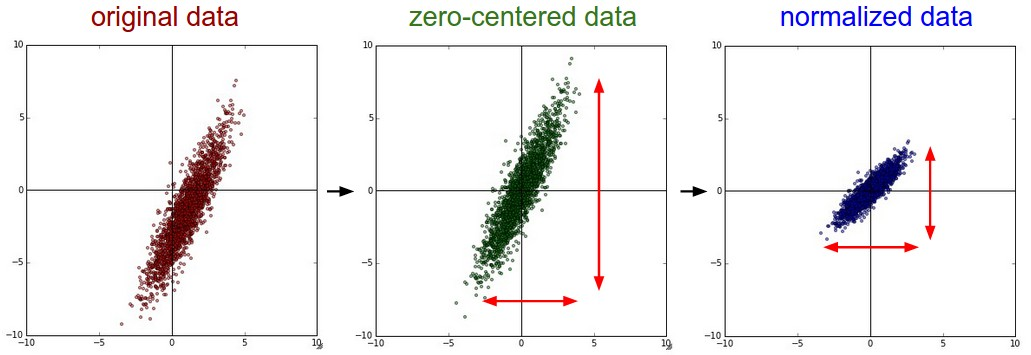
\includegraphics[width = 1.0\textwidth]{./Figures/normalization_1_prepro1.jpeg}
		\rule{35em}{0.5pt}
	\caption[Normalization]{Initialized weights of a neural network are usually randomly assigned between $-1$ and $1$. So on average a feature that has large values will contribute more to the weighted sum than another smaller scaled feature by virtue of having a greater product with the weighting. The arbitrary scaling of feature values should ideally not alter the results but it has been found to at best slow learning down, and at worst severely reduce model performance. Data will be normalized such that features are zero centred (centre graph), and the range of each feature made equivalent(right graph). By convention the range is between $-1$ and $1$}
	\label{fig:Normalization_2}
\end{figure}

\textit{Standardization} is another normalization method that not only rescales values over a similar range centered at the origin but to also have unit-variance as in Figure ~\ref{fig:Normalization_2}.
\be
x^\prime = \frac{x-\bar{x}}{\sigma}
\ee
where $\bar{x}$ is the mean of feature $x$ and $\sigma$ is the standard deviation.

In addition, feature variable may often be correlated.
This causes a problem for gradient descent, making optimization take longer\citep{featureScaling}.
Frequently a decorrelation method is used to transform the current set of features to a new set without correlation between variables.
Consider Figure ~\ref{fig:Normalization_3} where two features are strongly correlated with one another.
This can be treated simply with a linear transform to the feature vector which effectively rotates the axes to lie along the lines of correlated variables.
While most decorrelation algorithms are linear, non-linear decorrelation transforms do exist.
Decorrelation of features is often known as \textit{data whitening}
\begin{figure}[htbp]
	\centering
		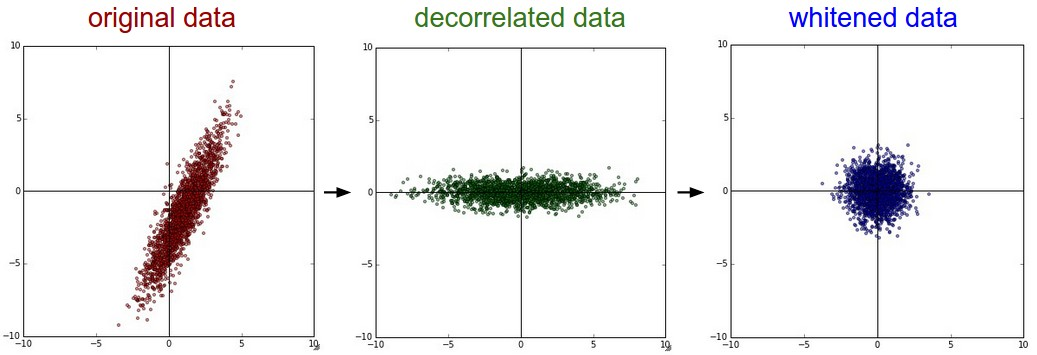
\includegraphics[width = 1.0\textwidth]{./Figures/normalization_2_prepro2.jpeg}
		\rule{35em}{0.5pt}
	\caption[Decorrelation]{Rescaling and centering data will still not be optimal for many machine learning algorithms. After zero centering, as in Figure \protect\ref{fig:Normalization_2}, there are still correlations in the data. That is, knowing the value of feature $x$ can inform you about the value of feature $y$. The slanted elliptical data distribution means the greater in value feature $x$ is, the more likely feature y will be larger. This is not ideal for learning because weightings on different features are now related which slows down the learning process and makes model interpretation more difficult. This issue can be dealt with by decorrelation. For linear correlations a rotation in feature space after zero-centering will work (center image). The features will still be on different scales. Decorrelation followed by rescaling the data (image on right) is known as \textit{data whitening}.}
	\label{fig:Normalization_3}
\end{figure}

%Batch Norm
So far we have spoken only of feature normalization, but neuron activations between layers may also be normalised in what is known as \textit{batch-normalization}.
Although inputs may be normalised, as the features are processed through the network, neuron activations may have gradually deviated from zero mean, unit-variance and become correlated in what is called \textit{co-variate shift}.
To correct for this Batch Normalization is often applied, which means for every batch of examples fed through the network a transformation is applied to the activations to keep the mean close to 0 and the standard deviation close to 1.
Batch Normalization ultimately results in faster, more accurate networks\citep{ioffe2015batch}.

\subsection{Learning Decay}
Throughout training, learning-rates tend to be either too small or too large for the local cost-surface.
Early in training a large step-size is desirable to quickly navigate down to a minima.
If the learning rate were to be smaller in these regions gradient descent can converge to the local minima.
Near the bottom a smaller step-size prevents over-shooting or oscillating over the minima.

Learning-decay tackles this by making the learning-rate, $\eta$, a function of the epoch number $i$
\be
\eta(i) = \eta_0 \frac{1}{(1 + \gamma i )}
\ee
where $\eta_0$ is the initial learning-rate and $\gamma$ is the decay constant.
Empirically learning decay has been shown to speed up learning and train more accurate models\citep{bengio2012practical}.
\begin{figure}[htbp]
	\centering
		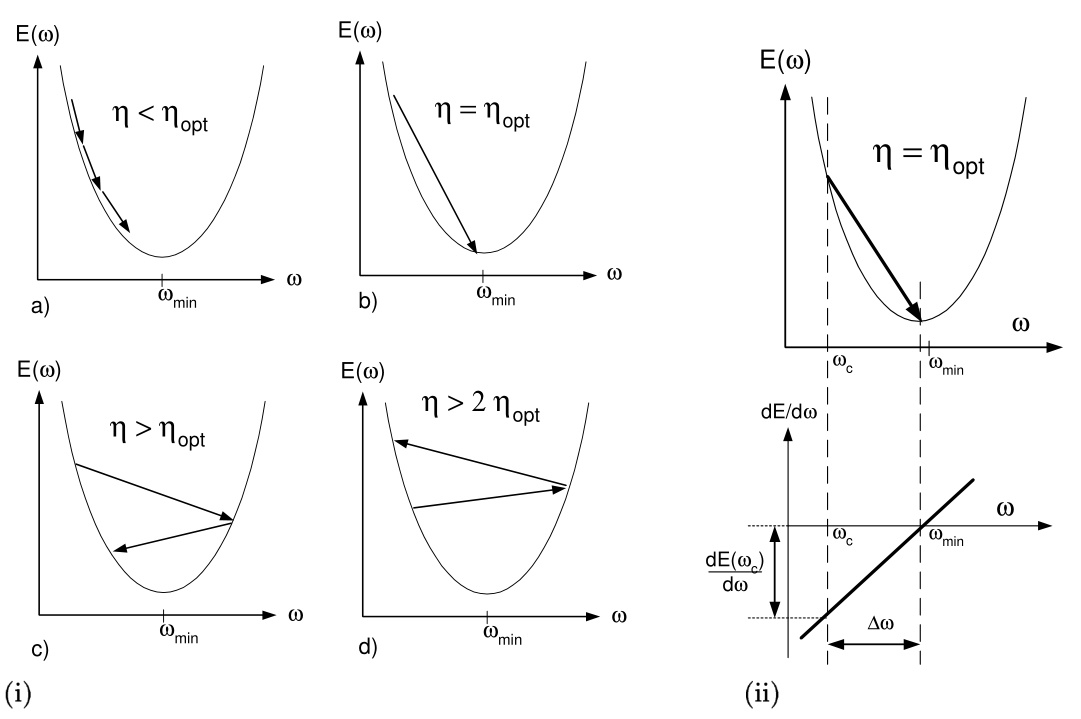
\includegraphics[width = 1.0\textwidth]{./Figures/efficient_backprop_learning_rate_issues.jpg}
		\rule{35em}{0.5pt}
	\caption[Optimum Learning Rates]{Where the gradient is negative the minima lies to the right, so adding the negative of the derivative multiplied by some constant $\eta$ will take the weight toward $\omega_{min}$. An optimal magnitude for $\eta$ will update the weight perfectly, as in (ii). This optimum value is usually not known ahead of time, so (i) explores the results of having a differing value. Where $\eta < \eta_{opt}$, see a), the weight updates will slowly approach the minima. Where $\eta$ is slightly larger than $\eta_{opt}$, see c), weight updates will oscillate over the minima. Too large a learning rate -  $\eta > 2\eta$ in the simplified case of a parabolic cost function - and the model weights will diverge.}
	\label{fig:Learning_rate_tuning}
\end{figure}


\subsection{Activation Functions}
Non-linear activation functions are used so as to be able to approximate non-linear relationships in the data\citep{bengio2009advances}.
A commonly used activation function is the sigmoid, shown in Figure ~\ref{fig:sigmoid}, which is given by the equation
\be
f(x) = \frac{1}{1 + e^{-x}}
\ee
and the hyperbolic tanh function\citep{bengio2009advances}.

Weights must be initialized such that activations are not saturated, especially in higher layers.
A saturated neuron is one that outputs a value near an activation function asymptote where the gradients are tiny.
should the neuron start, or become, saturated during training the back-propagated signal multiplied by the gradient will approach zero, effectively stopping the back-prolongation signal\citep{krizhevsky2012imagenet}.
\begin{figure}[htbp]
	\centering
		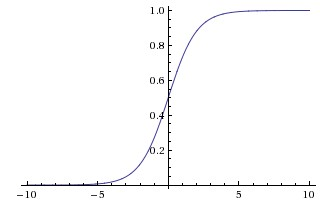
\includegraphics[width = 0.5\textwidth]{./Figures/sigmoid.jpeg}
		\rule{35em}{0.5pt}
	\caption[The sigmoid]{The ReLU funciton, $max(x,0)$, trains better performing networks significantly faster
	than the equivalent MLP using the $tanh$ or sigmoid activation functions.
	However where $x<0$ the neuron is \textit{dead}, or has a gradient of zero.}
	\label{fig:sigmoid}
\end{figure}


In theory, no non-linearity has more expressive power than any other, as long as they are continuous, bounded and monotonically increasing\citep{hornik1991approximation}.
However, the rectified linear unit (ReLU), shown in Figure ~\ref{fig:ReLU}, has been found to train faster\citep{nair2010rectified}.


Being a simple $max(0,x)$ operation, ReLUs quickly compute and are trained faster than both $sigmoidal$ and $tanh$ activations, see Figure ~\ref{fig:Relu_vs_sigmoidal} and Figure ~\ref{fig:Relu_vs_tanh}\citep{krizhevsky2012imagenet}.
In addition they do not require normalization to prevent saturation\citep{krizhevsky2012imagenet}.
If just a few examples produce a positive input to a ReLU, then learning will take place on that neuron.
However, ReLUs can die during training.
A dead ReLU is one in the $-\infty < x < 0$  region where the gradient is zero which prevents training of the neuron and layers below.
\begin{figure}[htbp]
	\centering
		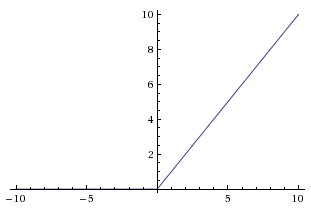
\includegraphics[width = 0.5\textwidth]{./Figures/relu.jpeg}
		\rule{35em}{0.5pt}
	\caption[The ReLU]{Of recent invent\citep{nair2010rectified} was the use of the ReLU activation function in MLPs. $g(z)_{ReLU} = max(0, z)$ has been found to train networks significantly faster which perform better than equivalent MLPs using sigmoidal activation functions..}
	\label{fig:ReLU}
\end{figure}
\begin{figure}[htbp]
	\centering
		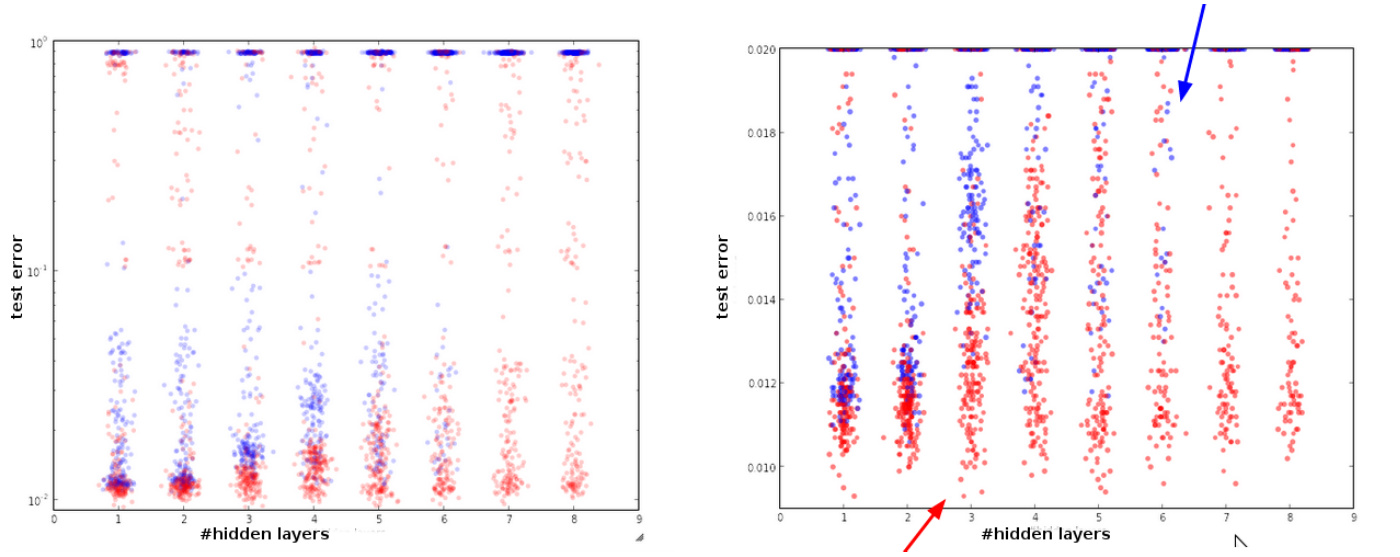
\includegraphics[width = 1.0\textwidth]{./Figures/effects_of_hyperpram_on_SGD_Bruel_relu_vs_sigmoidal.jpg}
		\rule{35em}{0.5pt}
	\caption[ReLU vs. Sigmoidal]{Models learned after being initialized with different weight parameters may differ in performance. One study\citep{nair2010rectified} explored the effects of using ReLU over the more traditional Sigmoidal activation functions. Many models of differing number of hidden layers and initialized weights were trained on the same data to see how activation functions affect performance. The graph on the left showing log(Test Error) vs. number of hidden layers shows a clear patter of ReLU models (in red) outperforming sigmoidal models (in blue) by two orders of magnitude at peak model performance densities. Zooming in on errors of order $10^{-2}$ on the right, the affect becomes more pronounced in larger models where ReLU models not only perform better on average but have error-rates no sigmoidal MLP ever achieves. }
	\label{fig:Relu_vs_sigmoidal}
\end{figure}
\begin{figure}[htbp]
	\centering
		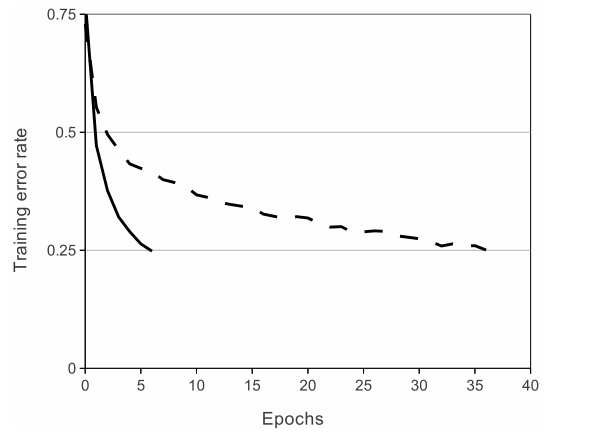
\includegraphics[width = 0.9\textwidth]{./Figures/Image_classification_with_DCNNS_relu_vs_tanh.jpg}
		\rule{35em}{0.5pt}
	\caption[ReLU vs tanh]{ReLU activation functions have been demonstrated to not only produce more accurate models but train significantly faster. Shown above the Training Error rate vs No. of Training Epochs. A four layer Neural Net achieves 25 \% training error rate on the popular image recognition CIFAR-10 data-set\citep{krizhevsky2009learning} six times faster than the equivalent network using $tanh(z)$ activation functions. Learning rates were optimized independently for each model so as to make training as fast as possible for that activation function. The magnitude of the effect will vary for different model architectures however models trained with ReLUs tend to consistently learn several times faster than their tanh or sigmoidal model equivalents. }
	\label{fig:Relu_vs_tanh}
\end{figure}



 \subsection{Weight Initialization}

Initial weight values have significant importance in training speed and accuracy\citep{lecun2012efficient}.
Weights cannot all be set the same value.
If all neurons where equally weighted they would produce the same output leading to the same gradients in back-propagation making training futile.
This is not true for biases which are generally set to $0$.
ReLU biases however are set to be a small positive value such as $0.01$ to ensure all ReLU activations are in the positive regime.

It has been discovered that output variance grows with the number of neuron inputs.
Training is more effective when the variance is normalized to $1$  with scaling by the $\sqrt{fan_{in}}$ (the number of inputs)\citep{neuralnetworkinitialization}.
\be
w = \frac{\Sigma(1,1)}{\sqrt{fan_{in}}}
\ee
where $fan_in$ is the number of inputs and $E$ is a Gaussian of mean $0$ and standard deviation $1$.

More recent analysis by Glorot et al\citep{glorot2010understanding} suggests weights should be sampled from the Gaussian $E(r,r)$
where $r = \sqrt{\frac{6}{fan_{in} + fan_{out}}}$ and $fan_{out}$ is the number of output neurons.

From a comparative study Larochelle et al. found that using the same neuron-count in each layer fares better than a decreasing or increasing neuron-count.
The first hidden layer cannot be too small else it cannot capture enough information from the input, but too many neurons risks over-fitting.
However. for most tasks an over complete first hidden layer works better than an under complete one.
A rule of thumb for the first hidden layer is $2n + 1$ where $n$ is the number of input features.

\subsection{GPU Speed Up}
%time-consuming 
%Parallizable
%CPU
%GPU
%Practical Implementations

%time-consuming 
When dealing with neural networks of many millions of parameters and tens of thousands of training samples the training process can take weeks.
Most of the training time is spent on matrix operations.
These are matrix-vector products, used in forward and back-propagation. and vector outer-products when calculating weight updates.

%Parallizable
Matrix-matrix multiplications can be done substantially faster than an equivalent sequence of matrix-vector products thanks to parallelism.
Firstly by smart caching mechanisms as implemented in the BLAS library, and thanks to parallelism\citep{wang2013augem}.
The speed-up is generally not in proportion to the number of cores used due to high data transfer and the associated latency\citep{ciresan2012multi}.
For small matrices the multi-core computations may take even longer than a single core because of this.
However, parallelism is more efficient with larger matrices.
Each neuron in a layer receives input as a weighted sum, or dot-product.
As such, neural networks are highly parallelizable by nature.
Entire training batches can be processed simultaneously.


In recent years GPU's decreased training times by some two-orders of magnitude compared to CPUs\citep{ciresan2012multi}.
The typical CUDA-capable\citep{cuda} GPU has several multi-processors(MP)\citep{chen2014big}; each of which contains several streaming multiprocessors (SMs) to form a building block.
Within each SM there are several stream processors (SP) that share control logic and global low-latency high bandwidth memory bank.
The high bandwidth comes at the cost of a small amount of RAM and lower clock speed.
GPU's typically have between 2-8Gb compared to up to a terabyte for a CPU.
Unfortunately information must be sent to the GPU by the CPU via the PCI-E connector which is slow and with large latency.
A GPU's architecture allows for thousand of threads, or processes, to run concurrently, shown in Figure ~\ref{fig:GPU_and_CPU}.
While CPUs are designed to handle general computing workloads, with units capable of processing high accuracy 64-bit floating point numbers, GPU's are less capable in the kinds of operations they can handle but can execute many at once making them excel at linear algebra and matrix multiplications.
\begin{figure}[htbp]
	\centering
		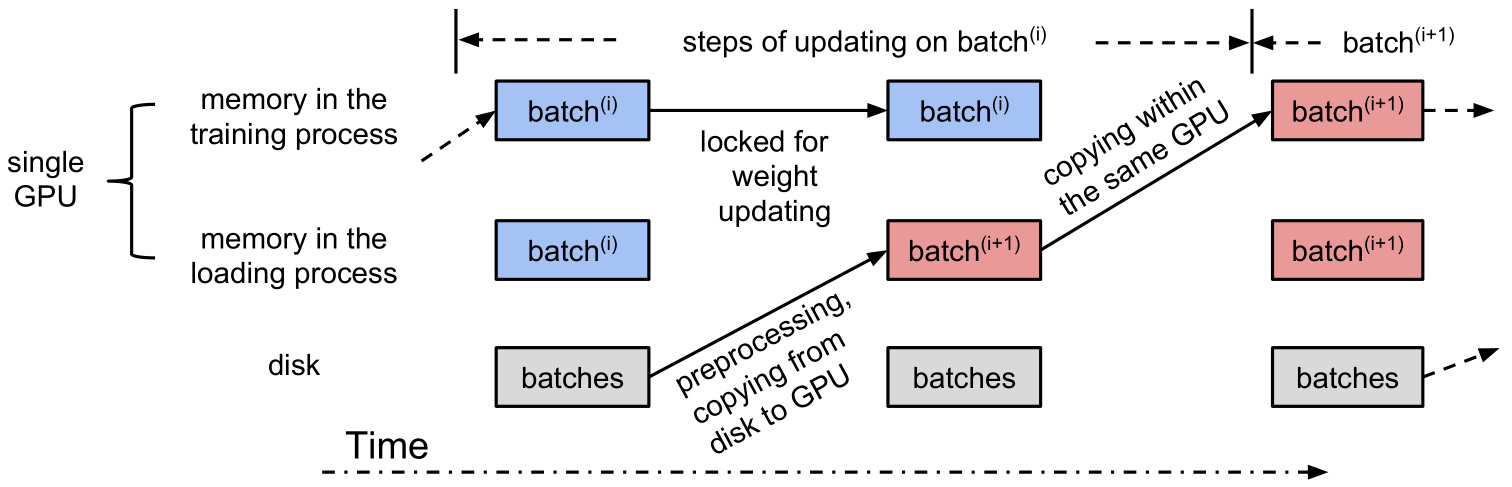
\includegraphics[width = 0.9\textwidth]{./Figures/Theano_based_large_scale_cisual_gpu_and_cpu_process.jpg}
		\rule{35em}{0.5pt}
	\caption[GPU Parallelized Training]{Graphics Processing Units (GPUs) excel at algebraic operations. GPUs were initially developed to use many cores for image-processing and the gaming industry. Despite each core being slower and with less allocated memory than a CPU, parallization allows for faster algebraic operations. Using a GPU, SGD on a GPU is handled like a production-line. Training batches are loaded onto the GPU (often pre-processed by the CPU). Then batches are simultaneously processed through the network to determine weight updates. Finally, model weights which are stored on the GPU are updated while the next training batch is loaded.
	\citep{neuralnetworkswebsite}}
	\label{fig:GPU_and_CPU}
\end{figure}


Unfortunately, programming GPUs is difficult, hard to optimize and requires specialized compilers.
Fortunately many software libraries, as in Figure ~\ref{fig:Theano}, have been developed at a higher level of abstraction to the GPU instructions.
For deep learning GPUs have become indispensable for model training in a reasonable time-frame. 
Together with libraries such as Theano and TensorFlow, models have been trained with over 100 million parameters.

\begin{figure}[htbp]
	\centering
		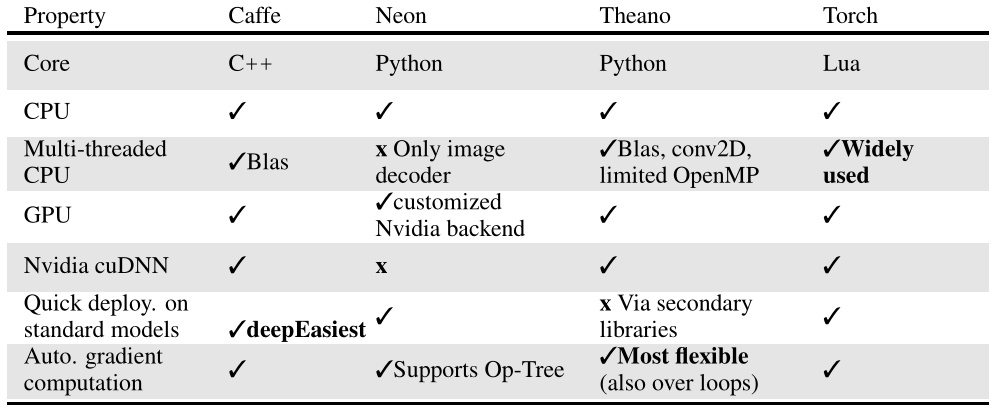
\includegraphics[width = 1.0\textwidth]{./Figures/theano_comparatives_study_of_cafe_neo_theano.jpg}
		\rule{35em}{0.5pt}
	\caption[Deep Learning Frameworks]{Several deep learning frameworks have been developed to accelerate model construction and training. Popular learning packages are shown above. The research in this thesis has been implemented using libraries built on top of the Python Theano framework. The open-source Theano, like several other frameworks, includes built in automatic gradient computation, commonly used functions, CPU multi-threading and GPU parallel processing on Nvidia hardware\citep{2016arXiv160502688short}.}
	\label{fig:Theano}
\end{figure}

  \section{Over/Under-fitting}
For a model to be useful it must generalize beyond the training data.
A model could have 100\% accuracy on the training data just by memorizing every example, but then it has not generalized at all. 
For an analogy; a student can learn to score 100\% on past paper questions if they appear in an exam but s/he has sacrificed general understanding for knowledge of particular questions and will likely perform poorly on unseen questions\citep{flach2012machine}.
S/he has \textit{over-fit} the training set of past papers but would not perform well on the test set (the exam), see Figure ~\ref{fig:Overfitting_2}.
\begin{figure}[htbp]
	\centering
		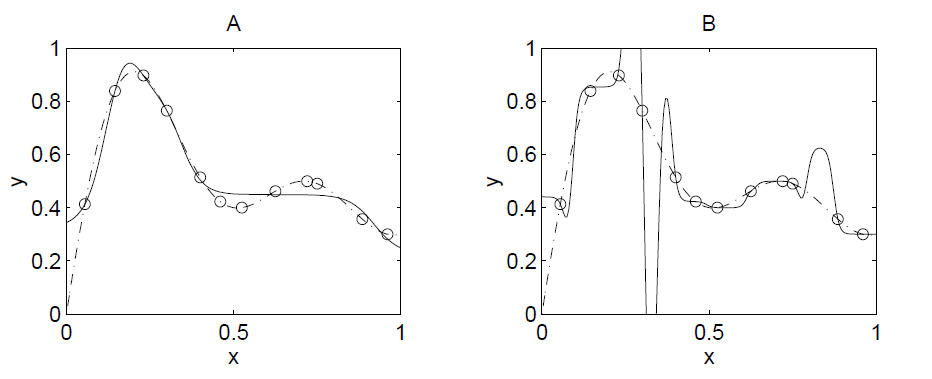
\includegraphics[width = 0.85\textwidth]{./Figures/An_intro_to_NNs_overfitting.jpg}
		\rule{35em}{0.5pt}
	\caption[Over-fitting]{A neural network is trained to predict $y$ from the $x$ feature based on the 12 examples, shown as circles. The dashed line shows the function from which the points were sampled. A) A network of 5 neurons in the hidden-layer is fitted to the data producing the function approximation shown by the solid line. The model fits well but appears to have some bias in the $0.4 < x < 0.9$ region where the model is insensitive to the variance within the training data. B) A network 20 hidden units is fitted. The significant number of parameters allows the model to fit perfectly, giving the correct prediction for every example feature. Bias is quite low in that the model is quite sensitive to variations within the data. However, variance is high as a small change in $x$ has extreme effects on the prediction. The model thus over-fits the training data and would not generalize to new data sampled from the original function.}
	\label{fig:Overfitting_2}
\end{figure}

This illustrates the need for splitting all the data into a \textit{training set} and \textit{test set}, illustrated by Figure ~\ref{fig:Training_and_Test}.
In order for this to work training and test samples must be representative of the underlying problem.
The test set must not be used in any way for training to remain an unbiased evaluation of the model's performance.
Should it be used for training, even indirectly, then the model can learn to fit the test set; like a student learning to pass a particular test and not have understanding of the subject.
This suggests that the model should not fully optimize performance on the training-set, see Figure ~\ref{fig:Peaking_effect}.
Over-fitting occurs more often in regression problems where the output is dependent on more than the information contained in the data set, such as environmental noise.
Should the model over-fit training data it is fitting to the noise and not the general trend.

\begin{figure}[htbp]
	\centering
		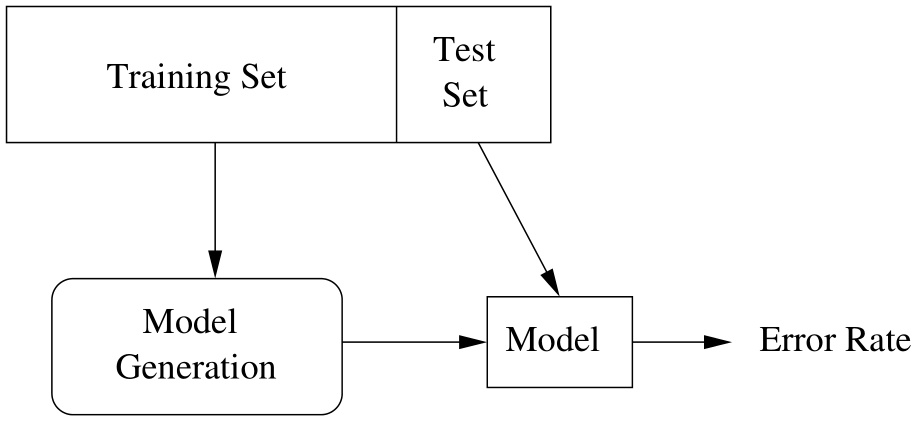
\includegraphics[width = 0.5\textwidth]{./Figures/training_and_test_sets_Mining.jpg}
		\rule{35em}{0.5pt}
	\caption[Model Training and Testing]{Model performance cannot be measured  with the training data as the result can be misleading. With enough degrees of freedom a model can fit the training data perfectly but generalize badly to unseen data. To avoid over-fitting the data is split into a training-set, and a test-set used only for an unbiased performance measure of the model.}
	\label{fig:Training_and_Test}
\end{figure}

\begin{figure}[htbp]
	\centering
		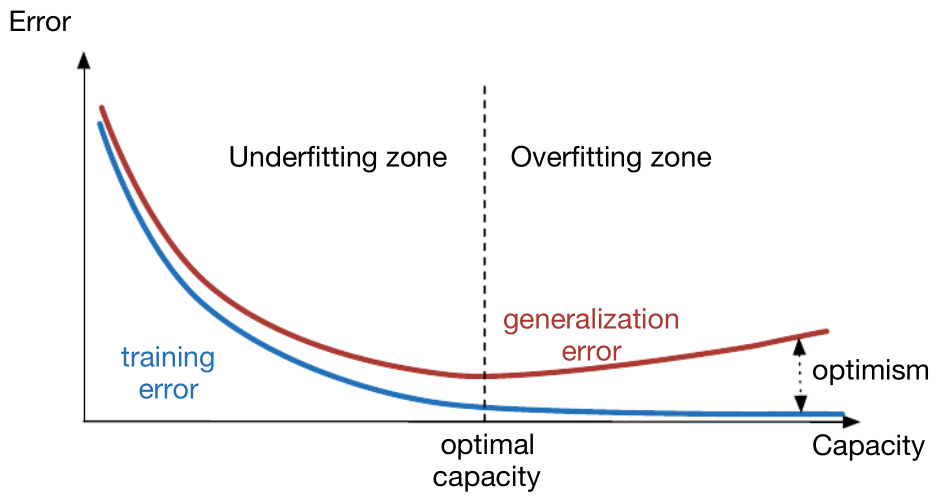
\includegraphics[width = 0.75\textwidth]{./Figures/overtraining_DL_textbook_6.jpg}
		\rule{35em}{0.5pt}
	\caption[Optimal Model Capacity]{The more parameters the more capacity (horizontal axis) a model has to fit training-data (bottom curve, blue) thereby reducing test error(top curve, red). Increasing capacity also expands the number of training samples a model can always fit. Training performance increases because the model fits the noise inherent to training data more than the general trend. Beyond the optimal capacity is the \textit{over-fitting regime}. Prior to the optimal model capacity, in the \textit{under-fitting regime}, there are not enough parameters to characterise the training data producing poor training and test performance results.}
	\label{fig:Peaking_effect}
\end{figure}

The `no free lunch' theorem formalized by Wolpert\citep{Wolpert96thelack} stipulates that no algorithm can beat random guessing over all possible functions to be learned seemingly supplanting machine learning altogether. 
However, real-world functions are not uniformly drawn from the set of all possible functions. 
Therefore it is reasonable to make assumptions that functions should be smooth, similar examples should have similar classes and simple functions are favoured over complex ones. 
Every algorithm must make assumptions beyond the data in order to generalize beyond the training data\citep{domingos2012few}.

Over and under-fitting can be described in term of \textit{bias} and \textit{variance}.
With too little complexity, loosely the number of parameters, a fitted model is \textit{biased}; insensitive to variation in the data.
For example a straight line fitted to points sampled from a sine function will not capture any of the oscillatory behaviour; the model has \textit{under-fit}.
In contrast, a highly complex function, as in the second frame of Figure ~\ref{fig:Overfitting_2}, can go through every point but introduces unnatural wiggles.
The model has high \textit{variance}; minor variations in the data would result in a very different model.
This illustrates the \textit{bias-variance dilemma}; too low complexity introduces systematic bias that no amount of data can resolve but too high and generalization is lost.

\subsection{Curse of Dimensionality}
Naively, intuitions formed in a 3D world suggest that the addition of features could only increase classifier performance.
However, with a large number of features potential benefit may be outweighed by the Curse of Dimensionality - a phrase coined by Bellman in 1961\citep{domingos2012few}.
Models generalize poorly in high dimensional data-sets for several reasons:

\begin{figure}[htbp]
	\centering
		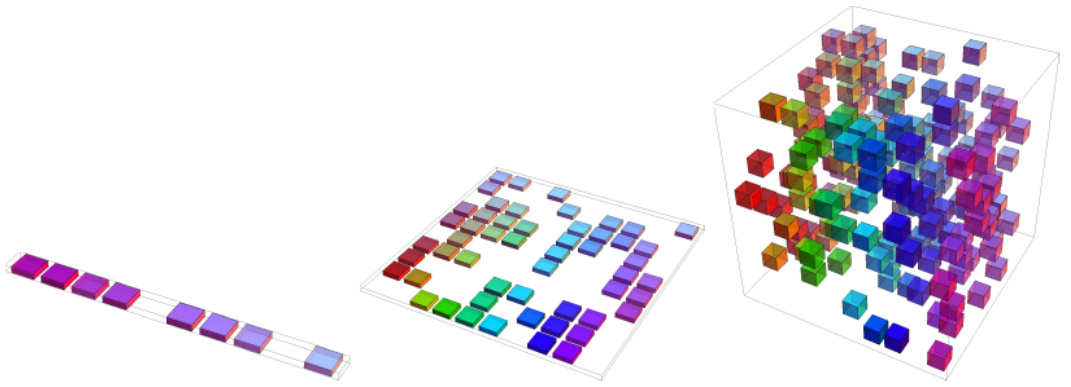
\includegraphics[width = 0.5\textwidth]{./Figures/Curse_of_dimentionality_DL_textbook_7.jpg}
		\rule{35em}{0.5pt}
	\caption[Curse of Dimensionality]{If 8 of 10 regions in a 1D feature space (leftmost image) are known; a density of 8/10 is sufficient to estimate values for the two unknown regions. In a 2D plane (center image) the number of regions grows to $10^2=100$. The number of samples needed to maintain the density is $0.8*10^2=80$. For a 3D feature-space (rightmost image) this escalates to 800 samples. In general the number of samples needed scales as $O(V^d)$ where $d$ is the number of dimensions and $V$ is the number of distinguishable regions per dimension.}
	\label{fig:Curse_of_dimensionality}
\end{figure}

\begin{enumerate}
\item When features are added to a fixed number of samples they cover a dwindling fraction of the feature-space.
If $n$ samples are required for an $R^1$ feature space to be considered dense, then $n^d$ samples are required to maintain the same density in $d$ dimensions, see Figure ~\ref{fig:Curse_of_dimensionality}.
The low data density in high dimensional space will require stronger and more accurate constraints\citep{cherkassky2007learning}.

\item Algorithms relying on similarity between samples (often a measure of the distance between points) break down.
Consider the K-nearest neighbour classifier. 
Unknown points are classified by comparing to the closest $K$ samples.
This is powerful in a densely packed low-dimensional space such as $R^2$.
However, with the addition of 98 irrelevant features ($R^100$), the irrelevant noise from the many features dominate the distance measure effectively making decisions random.

\item Even if all additional features are relevant, in a high dimensional space all examples can appear as nearest neighbours.
Consider the idealized case were examples are laid out on a regular grid.
In one dimension, the two nearest neighbours will lie on either side at the same distance from a sample $x_t$.
In two dimensions the four nearest neighbours lie at the corners of the square surrounding $x_t$. 
In general for a sample $x_t$ in $d$ dimensions the number of nearest neighbours is given by $2d$. 
In a high dimensional space so many samples can be considered nearest neighbours, effectively making the $K$ nearest neighbours random.


\item Objects in higher dimensional spaces have a larger amount of surface area for a given volume than objects in low dimensional spaces.
For example most of the volume of a multivariate Gaussian distribution comes not from near the mean (where the values are large) but much further out where the tails of the distribution are small but sweep into a much larger volume than near the core.
Put in another way, most of the volume of a higher dimensional orange comes not from the pulp but the thin sliver of skin far from the center.
it follows that in order to enclose even a small fraction of the data a large radius is required\citep{vladimir1998learning}.
The edge length of a unit-hypercube required to contain a fraction $p$ of the samples is given by 
\be
e_d(p) = p^{1/d}
\ee
where $d$ is the number of dimensions.
In order to enclose just 10 percent of the total data the edge length is $e_{10}(0.1) = 0.8$.
Therefore very large regions are required to capture a small amount the of the data making it difficult to provide a local estimate for high dimensional data.

\item Most samples will be closer to an edge that to any other sample.
For a scenario in which $n$ data points are uniformly distributed in a $d$ dimensional sphere of unit radius, the mean distance between the origin and the closest data point is
\be
D(d, n) = \left(1-\frac{1^{1/n}}{2}\right)^{1/d}
\ee
In a $200$ dimensional space with 200 data points this translates to a median distance of $D(10,200)\approx 0.57$.
The nearest point to the origin is over half the way from the origin to the radius, which is closer to the boundary of the data.
Most data points are outliers in their own projection.
This can be illustrated by the idea of standing at the end of a porcupine quill.
Every other quill will appear far away and clumped near the center.
This illustrates the difficulty in prediction of the label at a given point as any point will on average be closer to the edge than the training data point and so require extrapolation.

\end{enumerate}

There is some respite from the curse of dimensionality.
In general examples do not populate the feature space uniformly but are concentrated in a lower dimensional manifold.
For example k-nearest neighbours performs well for handwritten digit recognition though the feature space is large even for small images.
A $28\times 28$ pixel image equates to a feature space of $28^2 = 784$ dimensions, however the digits will only live in a much smaller sub-space of the full feature space.


\subsection{Data Augmentation}
Data Augmentation is using label-preserving transformations on already existing data to generate more 

Consider training a dogs and cats classifier.
If it so happens that many of the cats face toward the left the network may learn to only recognize those facing leftward facing cats and not 'realize' the class in not dependent on orientation.
To reduce over-fitting of this kind for images it is common practice to apply label-preserving transformations to already existing data to generate more. 
This is known as \textit{Data Augmentation}\citep{chatfield2014return} \citep{goyal2014object}\citep{krizhevsky2012imagenet}.
Using augmented data typically boosts performance by about 3 percent\citep{chatfield2015fly} even in large datasets, such as Galaxy Zoo\citep{lintott2008galaxy}\citep{goyal2014object}.
Commonly applied image transformations are skewing\citep{mo2012survey}, translation, reflection, brightness adjustment\citep{krizhevsky2012imagenet} and rotation\citep{chatfield2014return}.

The use of data augmentation does introduce a new problem.
If every image has many variations made the resulting dataset will be many times larger than the original.
Some datasets, such as ImageNet\citep{deng2012imagenet}, are already massive and it would be impractical to store all this data\citep{goyal2014object}.
This problem is treated by applying data augmentation on the fly while the original image is in memory, producing a temporary training batch before being discarded.
In many implementations image transformations are applied by the CPU while the GPU is training on the previous batch of images being even more economical with computing time.


\subsection{Regularization}
If the model has more parameters than necessary it will tend to over-fit the training data\citep{goyal2014object}.
\textit{Regularization} is a method of ensuring over-fitting does not occur even when the model is over-complex for the task.

\subsubsection{Weight Decay}
The idea behind \textit{weight decay}, also known as \textit{L2 regularization} is to add a \textit{regularization term} to the cost $C_0$ to obtain the modified cost $C$:
\be
C = C_0 + \frac{\lambda}{2n}\sum_\omega \omega^2
\label{eq:L2_cost}
\ee
where $\omega$ is the weights vector, $n$ the number of samples and $\lambda$ is a scaling constant.
All things being equal the network will now prefer to use small weights.

To see why this helps reduce over-fitting consider back-propagation with the modified cost function of Equation ~\ref{eq:L2_cost}.
The partial derivative used in back-propagation will be 
\be
\frac{\partial C}{\partial \omega} = \frac{\partial C_0}{\partial \omega} + \frac{\lambda}{n}\omega
\ee
and 
\be
\frac{\partial C}{\partial b} = \frac{\partial C_0}{\partial b} 
\ee
Substituting this into the weight update rules from Equation \ref{eq:updateEquation} we see
\be
b \rightarrow b - \eta \frac{C_0}{\partial b}
\ee
and 
\be
\omega \rightarrow \omega - \eta \frac{C_0}{\partial \omega} - \frac{\eta \lambda}{n}\omega = \left( 1 - \frac{\eta \lambda}{n}\right)\omega - \eta \frac{C_0}{\partial \omega}
\ee
The update rule for the biases is unchanged but the weights are rescaled by a factor of $1-\frac{\eta \lambda}{n}$ referred to as \textit{weight decay}.
This rescaling is what is refereed to as weight decay.
The first term favours few and small weights, however weight can still increase if it causes a decrease in the unregularized cost function\citep{bengio2012practical}.

In L1 regularization the added term is the sum of weight absolute values:
\be
C_0 + \frac{\lambda}{n}\sum_w |w|
\ee
Naturally this is similar to L2 in that the model prefers smaller and fewer weights.
To consider the difference between L1 and L2 regularization let us again consider the update rule with the modified cost function:
\be
\frac{\partial C}{\partial w} = \frac{\partial C_0}{\partial w} + \frac{\lambda}{n} sgn(w)
\ee
where $sgn(w)$ is the sign of $w$.
A small caveat is that the derivative $\partial C / \partial w$ is not defined when $w = 0$.
So in that case the standard update rule will be followed\citep{neuralnetworkswebsite}, equivalent to defining $sgn(0) = 0$.
The update rule is then
\be
w \rightarrow w - \frac{\eta \lambda}{n}sgn(w) - \eta \frac{\partial C_0}{\partial w}
\ee
Both L1 and L2 regularization shrink weights, however in L1 regularization weights are shrunk by a constant amount, whereas in L2 it is in proportion to $w$.
For a large weight the L1 regularization term $|w|$ is smaller than that of L2, and so the decay is less than for L2.
However when weights are small L1 will decay more than L2.
L1 therefore tends to result in a more sparse network; one with a small number of heavily weighted neurons with the rest close to zero.
Of course both types of regularization terms can be included in the model.
The linear combination of both L1 and L2 is termed an \textit{elastic net}.

\subsubsection{Drop-out}
\textit{Drop-out} is a powerful regularization method introduced by Hinton\citep{hinton2012improving} in 2012 which has been shown to work well for large neural nets.
\begin{figure}[htbp]
	\centering
		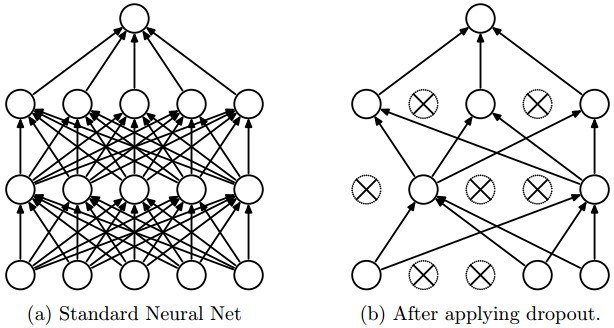
\includegraphics[width = 0.8\textwidth]{./Figures/dropout.jpeg}
		\rule{35em}{0.5pt}
	\caption[Drop-out]{Drop-out is an effective regularization method for MLPs. For every sample fed to the network only a fraction of randomly selected neurons may propagate the signal forward. This effectively creates a different architecture that shares weights with the original network. As a result neurons cannot rely on particular neurons from the layer below. This forces the network to generate a more robust representation of features from one layer to the next.}
	\label{fig:Dropout}
\end{figure}



In Drop-out a fraction $f$ of randomly selected neurons within a layer are prevented from propagating their signal to the layer above.
Neurons dropped out in this way contribute neither to forward-propagation nor back-propagation, as in Figure ~\ref{fig:Dropout}.
Instead of the layer computing $a=g(w.x)$ it now computes $a=m*\star g(w.x)$ where $m$ is a masking vector and $\star$ is the element-wise operator.
Activations of remaining neurons are multiplied by $1/f = 2$ to account for their being less active neurons\citep{goyal2014object}.
Now every time the input is injected, the neural network effectively samples from a different architecture sharing the same weights\citep{krizhevsky2012imagenet}.
As a result a neuron cannot rely on particular neurons firing from the layer below.
Instead individual neurons learn to detect more robust features, see Figure ~\ref{fig:Dropout_training}, which are helpful regardless of the large variety of internal contexts.

With Dropout the resulting model is the equivalent of training multiple networks and averaging their predictions.
Dropout may add up to a factor of two to training time but generates the equivalent of an ensemble in much less time\citep{krizhevsky2012imagenet}.

\begin{figure}[htbp]
	\centering
		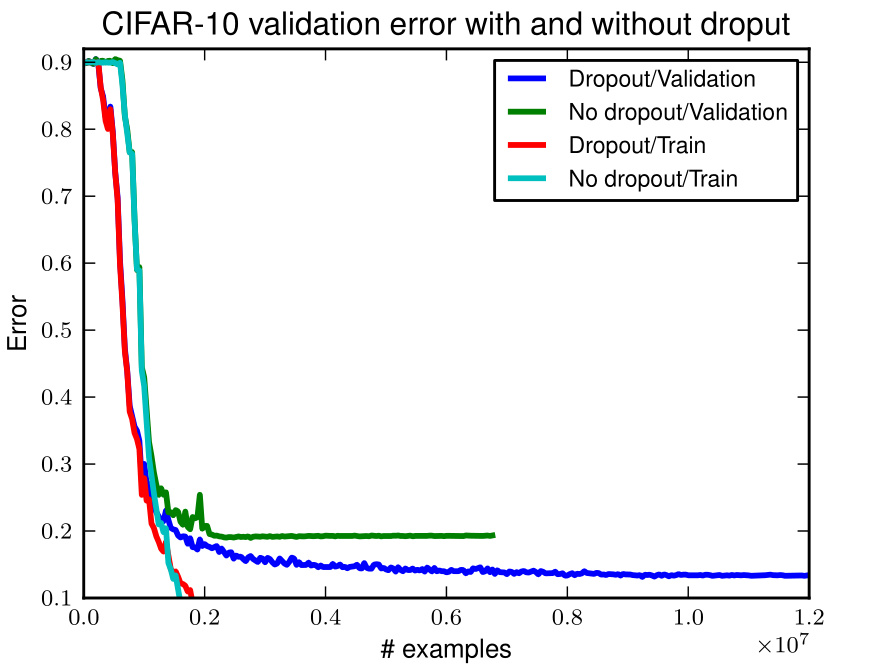
\includegraphics[width = 0.9\textwidth]{./Figures/training_with_dropout.jpg} %Dropout Benefits
		\rule{35em}{0.5pt}
	\caption[Drop-out Training]{A study\citep{wu2015towards} studied the effects of dropout on CNNs. Plotted above is model error vs the number of training samples. Error on the training set with drop-out (in red) is lower than without (in teal). The trend changes after $\approx 0.16\times 10^7$ training examples where the standard model over-fits the training set. Standard model validation error (in green) gets stuck in a local minima whereas the model with dropout (in blue) is continuously improving. This can be attributed to the changing network structure which alters the cost function and back-propagation signal. For few samples, < $1.6 \times 10^7$, performance is similar, however dropout helps prevent over-fitting.}
	\label{fig:Dropout_training}
\end{figure}

\subsubsection{Validation}
It is not enough to split the data into training and test sets to avoid over-fitting.
The practitioner could then tune model hyper-parameters by seeing which values lead to the best performance on the test set.
Doing this is indirectly training on the test data and no longer function as an independent source to evaluate the model\citep{witten2005data}.

This concern is what motivates the split of all the data into a training, validation and test set illustrated in Figure ~\ref{fig:Training_validation_and_Test}.
Typically the validation set is smaller than the training set so as to maximise training data.
Common practice is to split 70/30 for training and validation sets respectively.

\begin{figure}[htbp]
	\centering
		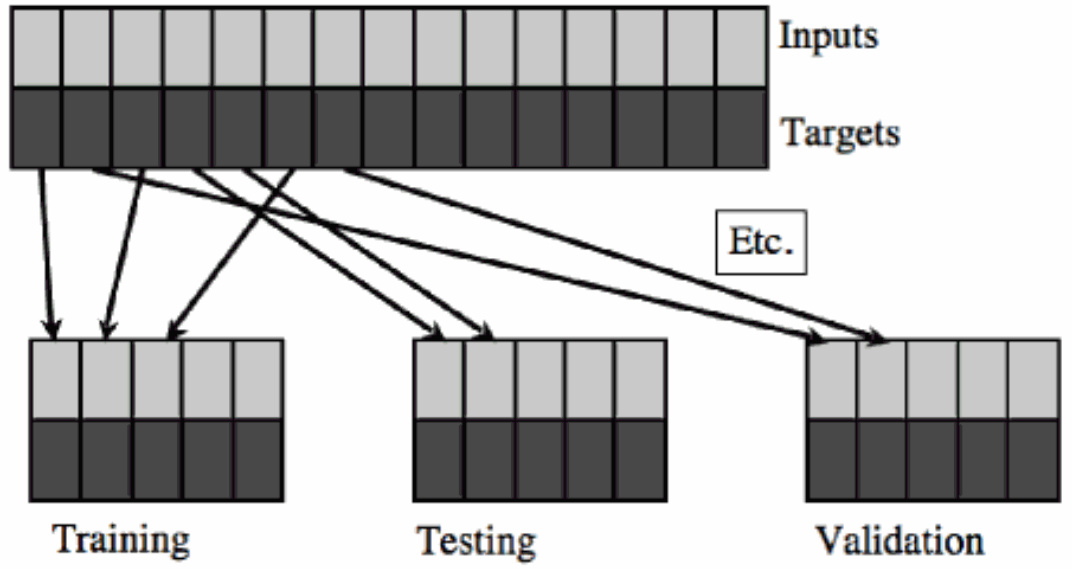
\includegraphics[width = 0.7\textwidth]{./Figures/training_validation_and_test_sets_ML_an_algorithmic_perspective.jpg}
		\rule{35em}{0.5pt}
	\caption[Validation]{If hyper-parameters are chosen based on test-set performance then the test-set is being indirectly fit to. This motivates splitting the data into three parts for training, validation and testing. The validation set is used for tuning hyper-parameters and the test set is used for measuring performance at the end.}
	\label{fig:Training_validation_and_Test}
\end{figure}

Hyper-parameters are tuned to maximise performance on the validation set and the completed model's performance is measured on the test set.\citep{barber2012bayesian}.

Once the hyper parameters have been selected and the model evaluated on the test set, it is possible to retrain the model on all the data.
With some well-behaved learning methods this is a reliable method to enhance the model\citep{witten2005data}.
However, to evaluate this new model a new source of test data must be created altogether.

\subsubsection{Cross Validation}
The more training data; the better the model. However, too little validation and test data makes for unreliable performance measures.
A commonly used method of K-fold cross-validation is used to handle the trade-off and is especially useful when there is little data altogether.

In K-fold cross validation the total data is split into $K$ equal sized partitions\citep{barber2012bayesian}.

See Figure ~\ref{fig:k_fold_validation_2} for an illustration of 5-fold cross validation.
\begin{figure}[htbp]
	\centering
		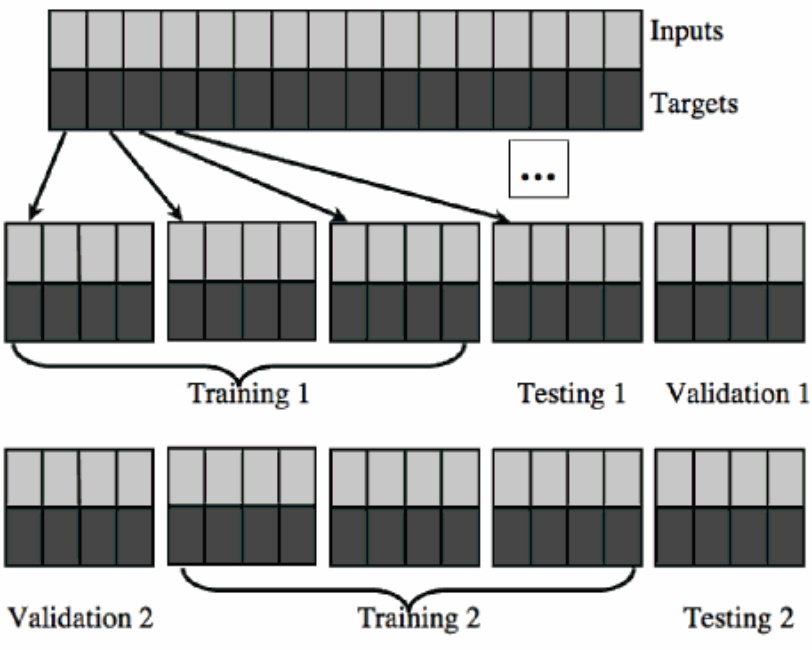
\includegraphics[width = 0.7\textwidth]{./Figures/ML_an_algorithmic_perspective_2_K_fold_validation.jpg}
		\rule{35em}{0.5pt}
	\caption[k-fold Validation]{For small datasets there may not be enough for training and validation sets. In K-fold cross validation the data is split in $K$ pieces to train $K$ different models each withholding a different piece for validation. The validation score is the average over all models.}
	\label{fig:k_fold_validation_2}
\end{figure}

The model is trained on the first $K-1$ partitions, leaving out the $K$'th partition as the validation set.
This is repeated for all $K$ combinations.
The validation performance is measured by taking the average performance of all $K$ models.
There is no objective rule what value to use for $K$. In practice it is common to use 10-fold validation.
An entirely unused test set must to used to measure the models final performance.

\subsubsection{Early Stopping}
%Early Stopping
If the model is over-complex it may over-fit if trained to convergence.
\textit{Early stopping}, see Figure ~\ref{fig:Overfitting_1}, is an inexpensive way to avoid over-fitting by stopping training ahead of convergence.
\begin{figure}[htbp]
	\centering
		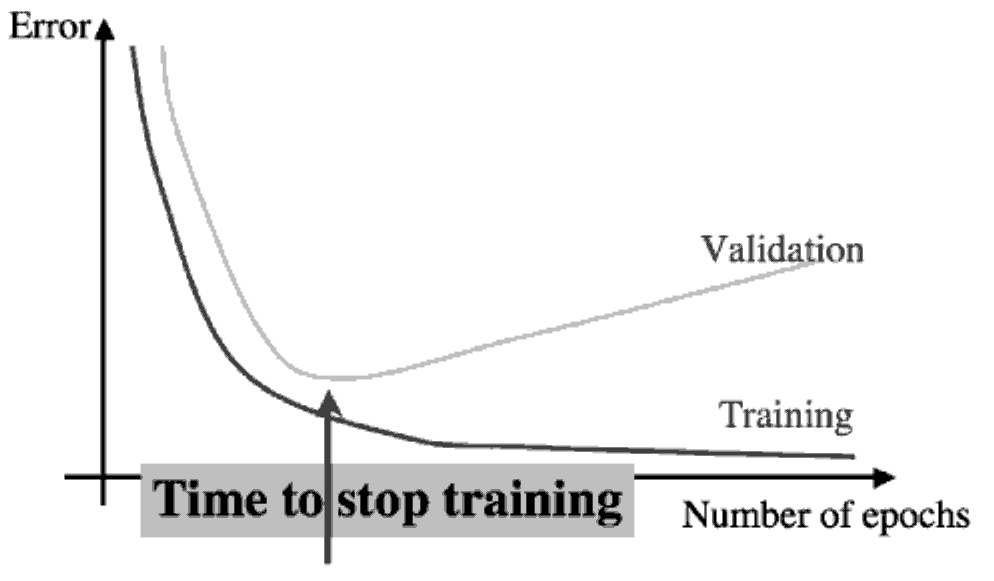
\includegraphics[width = 0.5\textwidth]{./Figures/machine_learning_an_aglorithmic_perspective_overfitting.jpg}
		\rule{35em}{0.5pt}
	\caption[Early Stopping]{\textit{Early-stopping} is a method of stopping training after a set amount of epochs to prevent over-fitting\citep{bengio2012practical}.}
	\label{fig:Overfitting_1}
\end{figure}

In one early stopping implementation the model is tested on the validation set after every $N$ updates.
Training is stopped when the model has performed best on the validation set\citep{bengio2012practical}.
Practically, training must go beyond the point of best validation error in order to detect the optimum epoch number.
Even if the model overshoots the optimum epoch-number, early-stopping will reduce over-fitting damage.
Unfortunately there is no a-priori  method to determine when to stop.
Instead, a few heuristics exist.
The one used in this thesis uses patience, which is the minimum number of training epoch before validation scoring which saves time in early training stages.
Once the threshold has been reached the validation score will be recorded after a further $N$ updates.
Should the new validation score be better than the previous training will continue for another $N$ updates otherwise training is halted.\citep{bergstra2010theano}\citep{bastien2012theano}.

\section{Deep Learning}\label{sec:deep_learning}
Machine learning methods typically use shallow-structured architectures.
These techniques have only one layer of non-linear feature transformations such as an ANN\citep{dengthree}.
Shallow architectures have proven to be successful in solving many simple or well-constrained problems, however their limited modelling and representational power is often insufficient for various real-world problems.
For example, image recognition\citep{dengthree} problems require the model to be insensitive to irrelevant variations, see Figure ~\ref{fig:Image_challenges}, such as lighting conditions, translations, rotations, pose, scale conformation and obstructions\citep{liu2014deep} while being sensitive to relevant variations such as distinguishing features of dog breeds.
A linear classifier would likely classify two different breeds of dogs as the same if they are in the same position and background.
Similarly a single breed of dog could be classified differently when in differing image contexts.

As a result shallow classifiers require smart feature extraction that solves the \textit{selectivity-invariance dilemma}; features must be selective of important variations and invariant to irrelevant ones.
Constructed features tend to be case-specific and require deep knowledge of the problem and data\citep{bengio2009advances}.
Depending on initial model performance features would then be redesigned in an iterative and time-consuming process, see Figure ~\ref{fig:deep_vs_classic_ml}.
\begin{figure}[htbp]
	\centering
		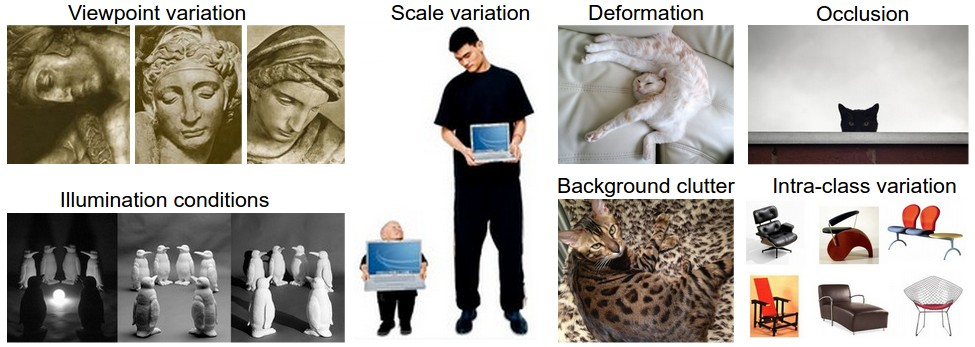
\includegraphics[width = 1.0\textwidth]{./Figures/challenges.jpeg}
		\rule{35em}{0.5pt}
	\caption[Image Recognition]{Image recognition is a difficult task as the very same object can appear with many irrelevant variations. For a model to be successful it must be impervious to these changes. For example, an object may vary in orientation(top left), lighting (bottom left), scale(middle) and distortion(one left of top right). In addition there may be contextual changes such as background clutter (one left of bottom right) and occlusion (top right). In addition the object class may vary in structure and colouring (bottom right) and yet still belong to the same class.}
	\label{fig:Image_challenges}
\end{figure}

\begin{figure}[htbp]
	\centering
		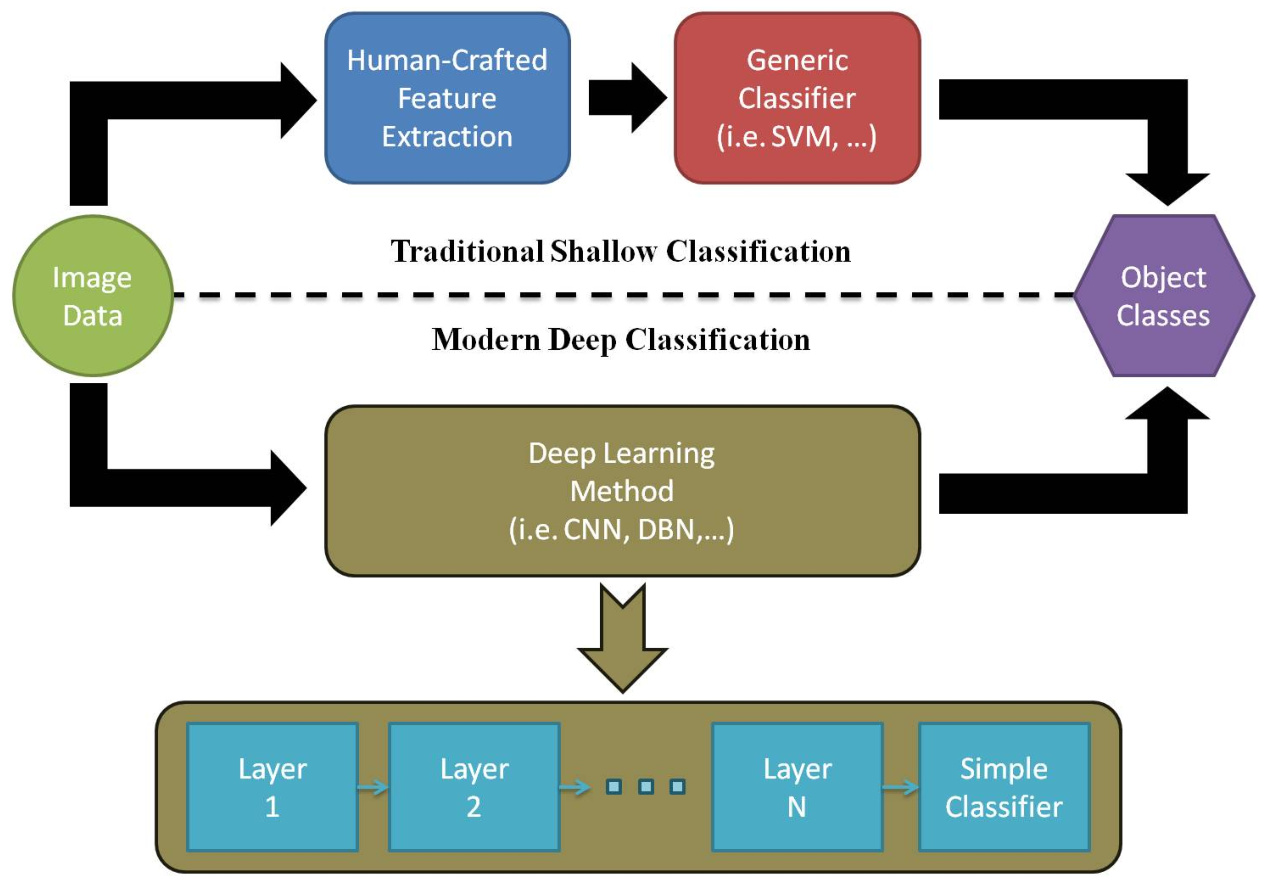
\includegraphics[width = 0.8\textwidth]{./Figures/deep_vs_classic_machine_leanring_sparse_coral_classification.jpg}
		\rule{35em}{0.5pt}
	\caption[Shallow vs. Deep Learning]{In shallow architectures features are manually created based on human analysis of the problem. Crafted features are then fed to one of many possible classifiers and tuned for peak performance. In contrast, no human-crafted features are necessary in deep-learning. Instead, the multi-layered architecture will learn the appropriate feature transformations to construct the most useful features. The final layer of the network presents these learned features to a simple classifier.}
	\label{fig:deep_vs_classic_ml}
\end{figure}

Speech exhibits hierarchical layered structure from the waveform level of sound to a linguistic level of speech\citep{baker2009variability}.
Similarly the visual systems are also hierarchical in nature.
Pixels may be assembled into edge-lets, edge-lets to motifs, motifs to parts, parts to objects, and finally objects to scenes\citep{lecun2010convolutional}.
This suggests that machine learning methods adopt hierarchical structure.
A \textit{deep-learning} architecture is a multilayer stack of simple modules which compute non-linear input-output mappings.
Each module in the stack performs a transformation on the input to increase selectivity and invariance of the feature-set.
See Figure ~\ref{fig:learning_complex_features} for an example of a multi-layered architecture developing better feature representations at every layer for facial recognition.
A deep architecture can eliminate feature extraction altogether\citep{lecun1995convolutional}.
The first few layers learn features directly from the input data, illustrated in Figure ~\ref{fig:first_layer_features}.
\begin{figure}[htbp]
	\centering
		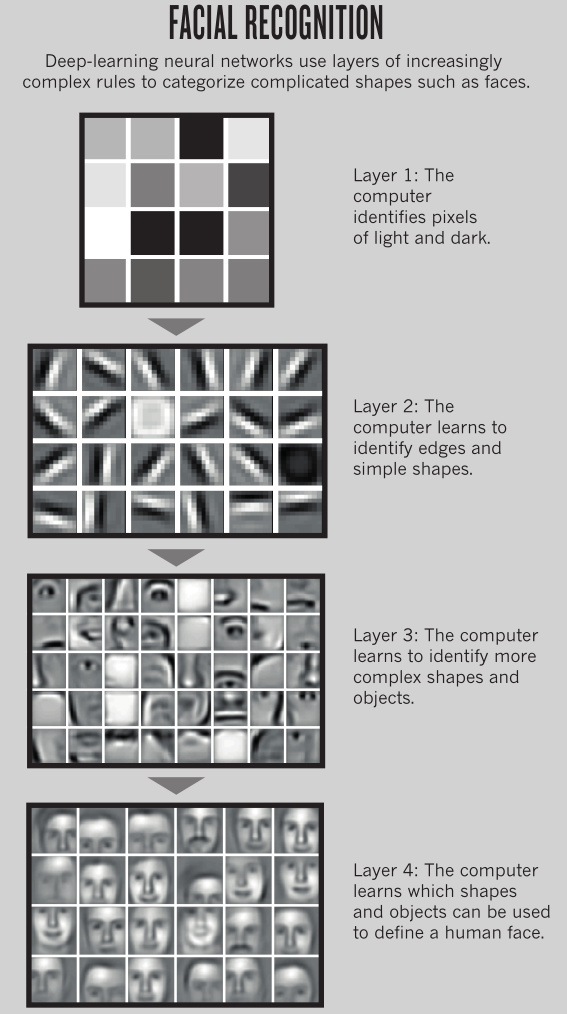
\includegraphics[width = 0.7\textwidth]{./Figures/learning_complex_features_the_learning_machine_nature.jpg}
		\rule{35em}{0.5pt}
	\caption[Learning Complex Features]{Deep Learning utilizes a multi-layered architecture to construct complex features of the input data. A model for facial recognition takes in pixel values as input. Layer 1 identifies light and dark pixels. Layer 2 learns to identify edges with different orientations and simple shapes from the output features of Layer 1. Layer 3 identifies more complex shapes and features from simpler shapes and edges. Layer 4 learns which complex shapes and objects define a human face. A face's image decomposed into its different parts and shapes can then be used to identify the person.}
	\label{fig:learning_complex_features}
\end{figure}
\begin{figure}[htbp]
	\centering
		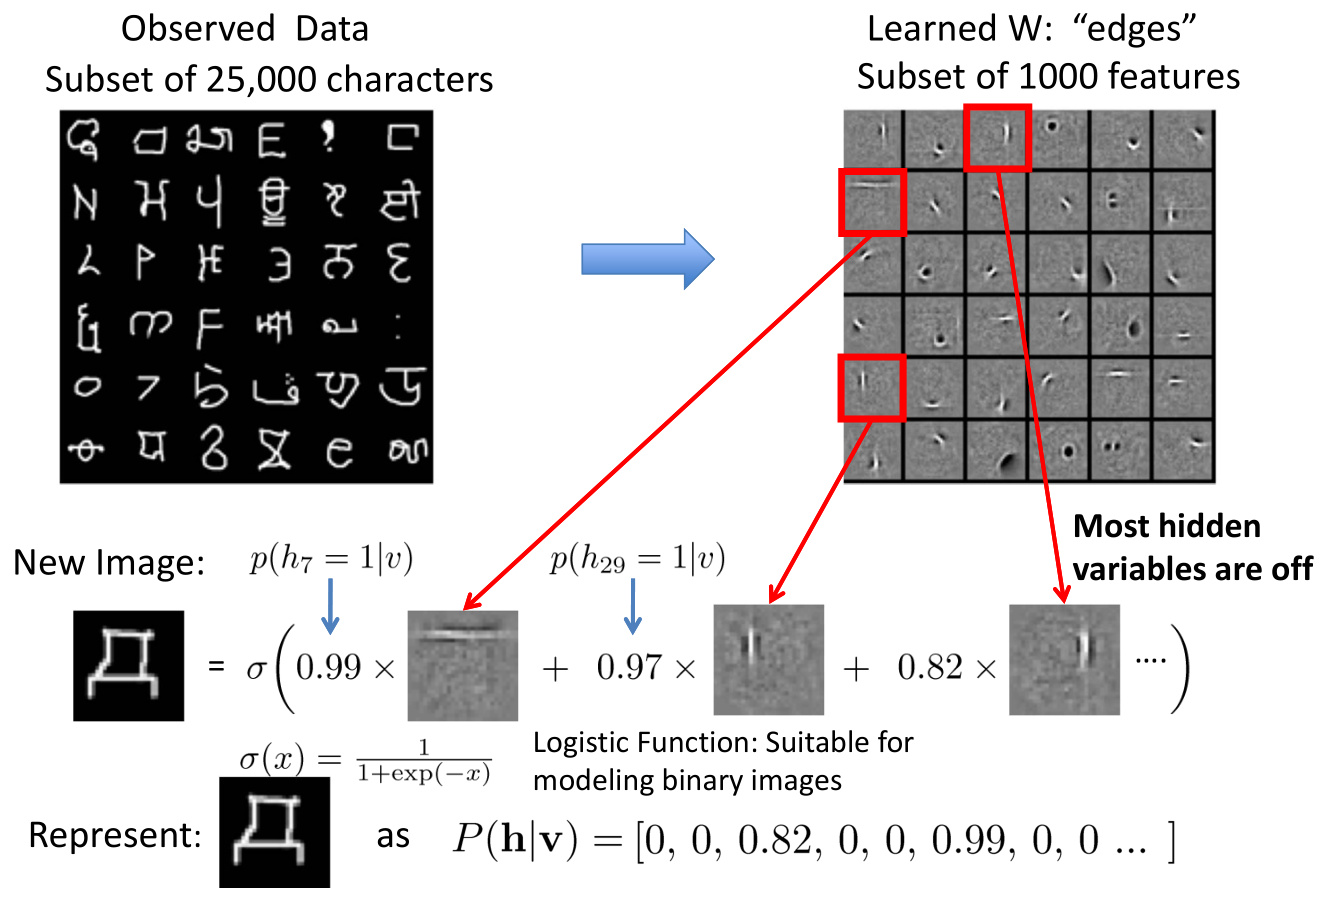
\includegraphics[width = 0.85\textwidth]{./Figures/Deep_Learning_Russ_Salakhutdinov_first_layer_features.jpg} %First layer visualization
		\rule{35em}{0.5pt}
	\caption[Learned Features]{Samples characters from a 25, 000 character dataset are shown above\citep{salakhutdinov2009deep}. Designing features that best capture information relating to these characters would take plenty work and insight. Deep Learning can learn complex features directly from the data. On the right we can see a sample of what image characteristics provide the most activation to neurons higher up in the network. The network has learned to use edge detectors at different locations and orientations. Now a character can be decomposed into 1000 coefficients of the feature maps rather than manual feature construction.}
	\label{fig:first_layer_features}
\end{figure}

\textit{Deep Learning} (DL) algorithms are inspired by the human brain\citep{mo2012survey}\citep{chen2014big}.
The brain quickly processes complex data, learns in different domains and solves complicated tasks.
DL aims to deal with high-dimensional data efficiently and quickly; performing complicated tasks such as image and sound recognition.
As Bengio and Lecun put it, ``Deep architectures are compositions of many layers of adaptive non-linear components, in other words, they are cascades of parametrized non-linear modules that contain trainable parameters at all levels''\citep{bengio2007scaling}.
DL refers to supervised or unsupervised algorithms with many layers of information processing that learn hierarchical representations of the data\citep{chen2014big}\citep{dengthree}.
While there were multiple deep architectures before 2006, almost none were successful is terms of accuracy and efficiency with the exception of Convolutional Neural Networks (CNNs)\citep{lecun1995convolutional}. 

DL methods have had many successful applications.
Visual document analysis\citep{simard2003best}\citep{karnowski2010deep}, facial\citep{le2013building}\citep{farfade2015multi} and speech recognition, natural language processing, human action recognition\citep{ji20133d}\citep{mo2012survey}, facial location \citep{liu2014deep}, image semantic discovery\citep{liu2014deep}, image compression\citep{goyal2014object}, collaborative filtering\citep{chen2014big}, and Medical Diagnosis\citep{goyal2014object}.
Companies such as Google, IBM, Apple and Facebook have all been aggressively pursuing DL projects.
Google has used DL for voice recognition, Street View and image recognition; Microsoft for their real-time language translation in Bing voice search\citep{dahl2011large}, and IBM for their Jeopardy winning Watson\citep{ferrucci2013watson}\citep{chen2014big}.
Siri, the iOS assistant, gives weather reports, provides news, answers questions and gives reminders all with the power of DL\citep{chen2014big}.
The recent enthusiasm for DL is largely a result of increased hardware capabilities, specifically GPUs, cheaper computing equipment and recent advances in research\citep{dengthree}.
As Big Data only gets bigger, DL will play a larger role in predictive analytics especially considering the advances in computing power and use of parallel processing in GPUs\citep{chen2014big}.

Bengio and Lecun proposed the following requirements for a successful DL implementation\citep{bengio2007scaling} \citep{bengio2009learning}\citep{chen2014big}.
The algorithm must:

\begin{enumerate}
\item function with a large range of architectures.
\item handle deep architectures, and manipulate intermediate features with many levels of non-linear transformations.
\item sample from a large space of possible functions with many millions of parameters.
\item scale efficiently with the number of parameters and samples. This prohibits algorithms that iterate many times over the data.
\item discover multi-use concepts(multi-task learning) and may use unlabelled data.
\end{enumerate}

\subsection{Convolutional Neural Networks}

\subsubsection{Introduction}

The Universal Approximation theorem by Hornik\citep{hornik1991approximation} states that a neural network with a single hidden layer can model any continuous function.
However, Bengio\citep{bengio2009learning} showed that a shallow network would require an exponentially large number of neurons when compared to a Deep Neural Network(DNN) with many hidden layers.
Recently in 2014, Romero\citep{romero2014fitnets} and Ba and Caruana\citep{ba2014deep} showed that a deeper neural network can be trained to perform much better than a comparatively shallow one.
However, DNNs typically require huge computational resources that make their training and real-time application difficult to implement\citep{goyal2014object},

DNNs face several challenges\citep{mo2012survey}:
\begin{enumerate}
\item DNN's cannot train on unlabelled data, which greatly outnumbers labelled data.
\item Back-propagation correction signals get severely weakened travelling through the neural network.
This results in layers near the top being altered, but layers near the bottom are largely unaffected; the \textit{gradient dilution problem}\citep{bengio2009learning}.
\item Learning is very slow for networks of many layers due to the many millions of weighted sums, activations and back-propagation signals that need to be computed.
\item The network is likely to end up in a poor local minima rather than the global one.
The severity of poor local minima increases significantly as network depth increases\citep{dengthree}.
\item The main deficiency of unstructured nets is their lack of built-in invariance with respect to translations and distortions\citep{lecun1995convolutional}.
For example, digits may appear with differing slants, sizes and positions.
Words are spoken with varying pitch, speed and intonation.
In principle, a sufficiently large network can learn to be invariant to such transformations, however that will likely result in multiple units with identical weight patterns and the number of training instances required is very large\citep{lecun1995convolutional}.
\item Due to the input data being vectorised and fed to the first layer, the topology of the input is ignored.
This is contrary to the fact that spectral representation of speech and images have strong local 2D structures and times series strong 1D local structure.
For example, pixels that are spatially or temporally nearby are highly correlated\citep{lecun1995convolutional}.
\item The large number of trainable parameters allows for easy over-fitting.
\end{enumerate}

In 1962 Hubel and Wiesels' revealed from studies of cats' primary visual cortex\citep{lecun1995convolutional}\citep{bengio2009advances}\citep{goyal2014object} that there is a hierarchy operating within neurons of the visual cortex in living organisms.
Simple neurons in the up-most layer connect to a small region of complex neurons below\citep{gabor1946theory}.
The first neural nets based on this insight were Fukushima's Neocognition and Lecun's Net-3\citep{bengio2009advances}.
In such an architecture the lower layer is divided into a smaller number of regions called \textit{Receptive Fields}, each of which is mapped to a single of the layer above\citep{bengio2009advances}.
The connection is called a \textit{feature extractor}.
Many such feature extractors are applied to the same receptive field generating a corresponding feature vector.

Advantages for this architecture include\citep{lecun2015deep}:
\begin{enumerate}
\item Sparse Connectivity - Rather than connect an entire layer to the layer above, each receptive field is connected to a single neuron, see Figure ~\ref{fig:sparse_vs_fully_connected}.
This significantly reduces the number of parameters which makes training much easier\citep{bengio2009advances} and faster.
Trials have consistently shown, see Figure ~\ref{fig:Sparsity}, that sparsely connected networks outperform their fully connected versions.
\item Shared weights - This means each receptive field is connected to the upper layer by an identical set of weights\citep{krizhevsky2012imagenet}\citep{lecun1995convolutional}, see Figure ~\ref{fig:parameter_sharing}.
Elementary feature detectors useful in one part of the image are likely to be useful everywhere\citep{lecun1995convolutional}.
This is a strong, yet justified, assumption in the locality of pixel dependencies.
This again significantly reduces the number of parameters that need to be learned improving training\citep{mo2012survey}\citep{bengio2009advances} and model generalization while the best possible theoretical performance is only slightly worse than for a fully connected DNN\citep{krizhevsky2012imagenet}\citep{lecun1995convolutional}.
\item Sub-sampling - Between layers input data is sub-sampled in what is known as \textit{pooling} which significantly reduces the number of parameters and computations required\citep{bengio2009advances}\citep{chen2014big}\citep{ciresan2012multi}.
\item Deep Architecture  - The many layered architecture allows for extracting highly non-linear and robust features.
\end{enumerate}
\begin{figure}[htbp]
	\centering
		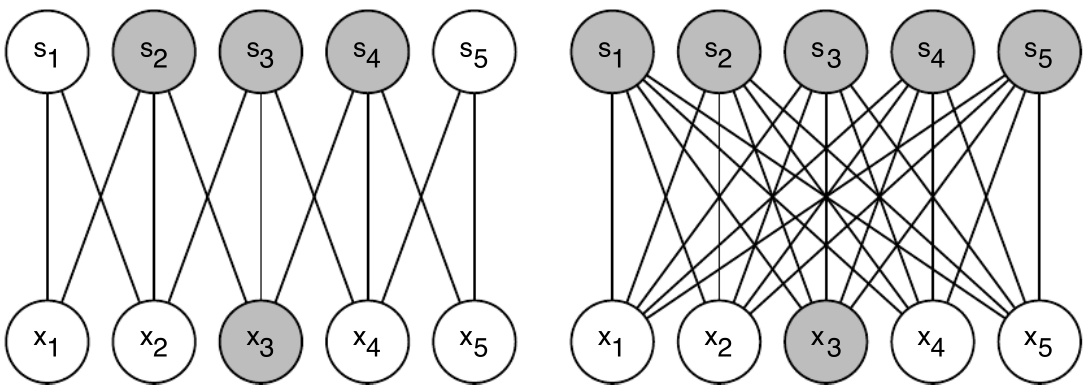
\includegraphics[width = 0.5\textwidth]{./Figures/Spars_verse_fully_connected_DL_textbook.jpg} %Sparse Connections
		\rule{35em}{0.5pt}
	\caption[Sparse Connectivity]{MLPs with full-connectivity between layers $L_1$ and $L_2$ have $N_1 \star N_2$ parameters, where $N_i$ is the number of neurons in layer $i$. For two layers of 5 neurons each there will be $ 5 \times 5 = 25$ connections. However, if neurons in $L_2$ may only connect to a local subset of neurons there is a significant reduction in the number of parameters $ 3 \times 3 + 2 \times 2 = 13 $ connections.}
	\label{fig:sparse_vs_fully_connected}
\end{figure}
\begin{figure}[htbp]
	\centering
		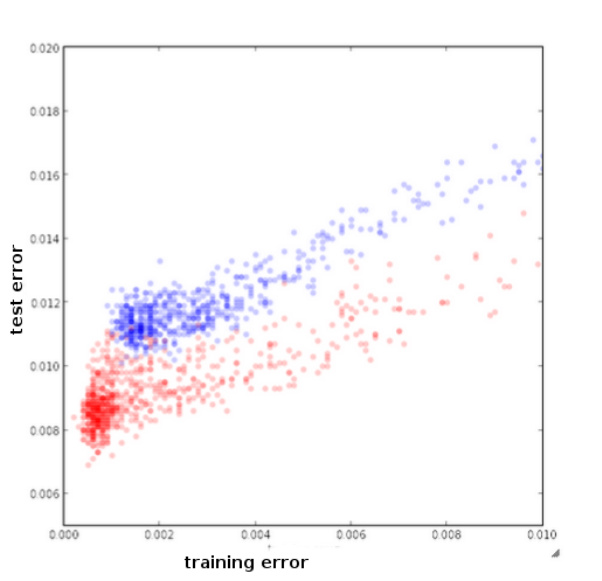
\includegraphics[width = 1.0\textwidth]{./Figures/effects_of_hyperpram_on_SGD_Bruel_CNN_Sparsity.jpg} %CNN vs Fully connected
		\rule{35em}{0.5pt}
	\caption[CNN vs. Fully Connected]{Naively on would think a fully connected network should outperform a CNN. However, the sparse and shared connections ensure back-propagation signals do not disappear and improves invariance to label-preserving transformations. The scatter plot depicts converged model performance on test and training sets for both CNNs (in red) and MLPs (in blue). Points to the bottom left are preferable as they have both low training and test errors. CNNs consistently outperform their fully connected counterparts in both test and training error for the majority of random parameter initializations.}
	\label{fig:Sparsity}
\end{figure}
\begin{figure}[htbp]
		\centering
			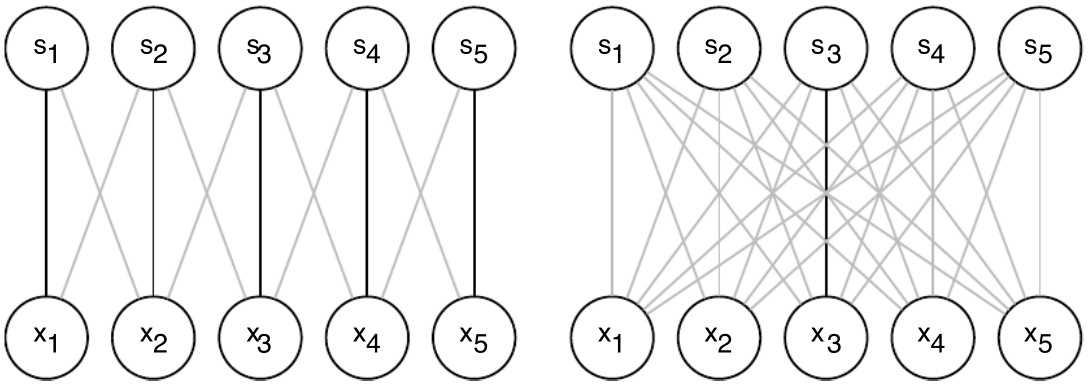
\includegraphics[width = 0.9\textwidth]{./Figures/parameter_sharing_DL_textbook_2.jpg} %parameter sharing
			\rule{35em}{0.5pt}
		\caption[Parameter Sharing]{The network on the left makes use of parameter-sharing; bold lines show all the connections equal to the $x_3$ to $s_3$ weight. In total there are three unique weights. In contrast, the fully-connected network on the right has $5^2 = 25$ unique weights.}
		\label{fig:parameter_sharing}
\end{figure}

The resulting model, a \textit{Convolutional Neural Network}(CNN)\citep{dengthree}, learns hierarchical representations of the data using local receptive fields, shared weights and sub-sampling and is more resilient to variations within the data\citep{lecun2010convolutional}.

A typical CNN is composed of many layers; some for feature representations, known as \textit{feature maps}, and others as conventional neural networks.
The input and output of each stage is a set of matrices called feature maps.
In the case of a colour image, the input to the first layer can be thought of as an input of three feature maps; each a 2D array containing a colour channel of the image.
For audio input this is a 1D feature map, for video or a volumetric image (such as an MRI) the feature maps are 3D.
Each feature map represents a particular feature at all locations over the image, such as vertical lines.
A CNN alternates between two types of layers, \textit{convolutional} and \textit{pooling}, which together make up a single CNN stage\citep{chen2014big}.
There will be several such stages followed by a set of fully connected neurons to form a classification module\citep{lecun2010convolutional}.

CNNs have been successfully used in many commercial projects including Optical Character Recognition, handwriting recognition (including Arabic and Chinese),video surveillance\citep{bengio2009advances} and speech recognition\citep{dengthree}\citep{haffner1998high}\citep{krizhevsky2012imagenet}\citep{donahue2014decaf}\citep{simonyan2014very}\citep{abdel2012applying}\citep{sainath2013learning}.
The first commercial deployment was for check reading ATM machines in Europe in 1993\citep{bengio2009advances}.

\subsubsection{Convolution}
Each convolutional layer constructs several feature maps convolving input with different feature filters (weight matrices).
The value of each pixel in the feature map is the result of connecting a small defined region of the input below to a single neuron above, refer to Figure ~\ref{fig:CNN_2}.
Weights used in this connection are the filter which will move over the whole image to generate different pixels in the above feature map.
The application of several different filters will produce the same number of feature maps\citep{lecun2010convolutional}\citep{mo2012survey}.
Expressed as a vector equation with pixel location indices suppressed,
\be
y_j^{(l)} = f\left(\sum_i K_{ij} \otimes x_i^{(l - 1)} + b_j \right)
\ee
where $Y_j^{(l)}$ is the $j$-th feature map of the $l$-th convolution layer, and $f$ is a non-linear activation function\citep{lecun2010convolutional}\citep{mo2012survey}\citep{chen2014big}.
$K_{ij}$ is a trainable filter (or \textit{kernel}) that convolves with feature map $x_i^{(l - 1)}$ from the previous layer to produce a new feature map in the current layer as illustrated in Figure ~\ref{fig:Convolution}.
Symbol $\otimes$ is the discrete convolution operator and $b_j$ the bias term.
Each filter $K_{ij}$ can connect to all or a portion of the feature maps from the previous layer.
The weights $K_ij$ are trained via back propagation.

\begin{figure}[htbp]
	\centering
		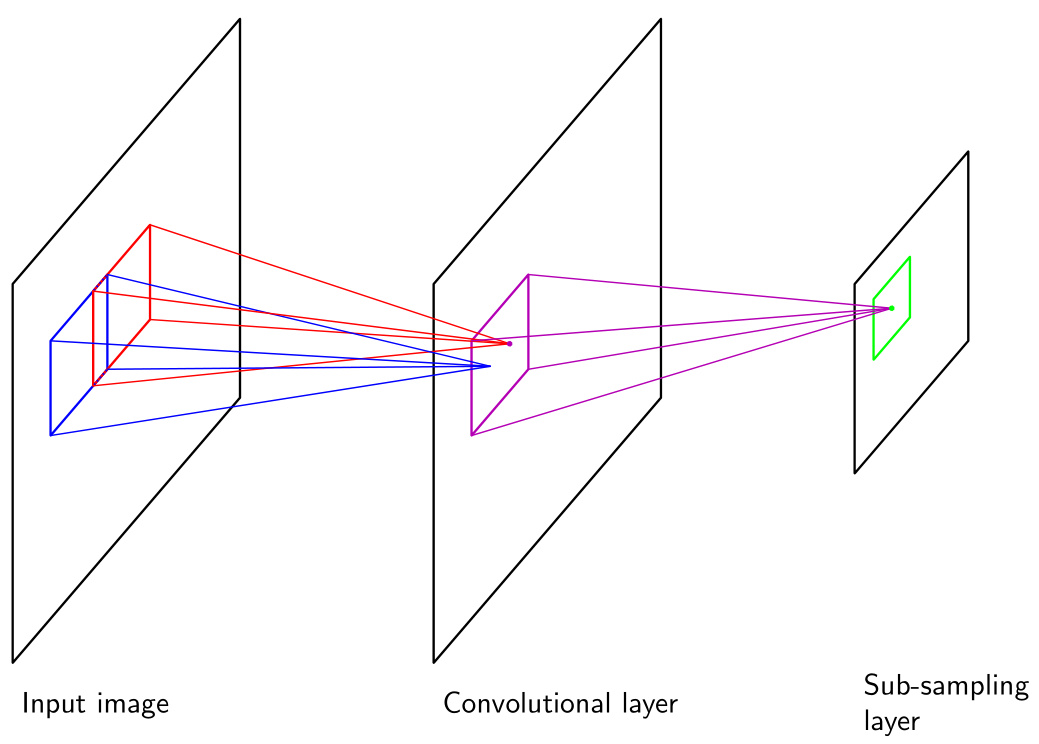
\includegraphics[width = 1.0\textwidth]{./Figures/pattern_recognition_and_machine_learning_CNN.jpg} % SIngle CCN layer
		\rule{35em}{0.5pt}
	\caption[A CNN Layer]{A CNN is made up of many alternating convolution and pooling layers. Each convolutional layer can make use of many kernels. The output feature maps are then subjected to a pooling or sub-sampling layer. A convolution and pooling stack together form one of several successive layers of a CNN.}
	\label{fig:CNN_2}
\end{figure}
\begin{figure}[htbp]
	\centering
		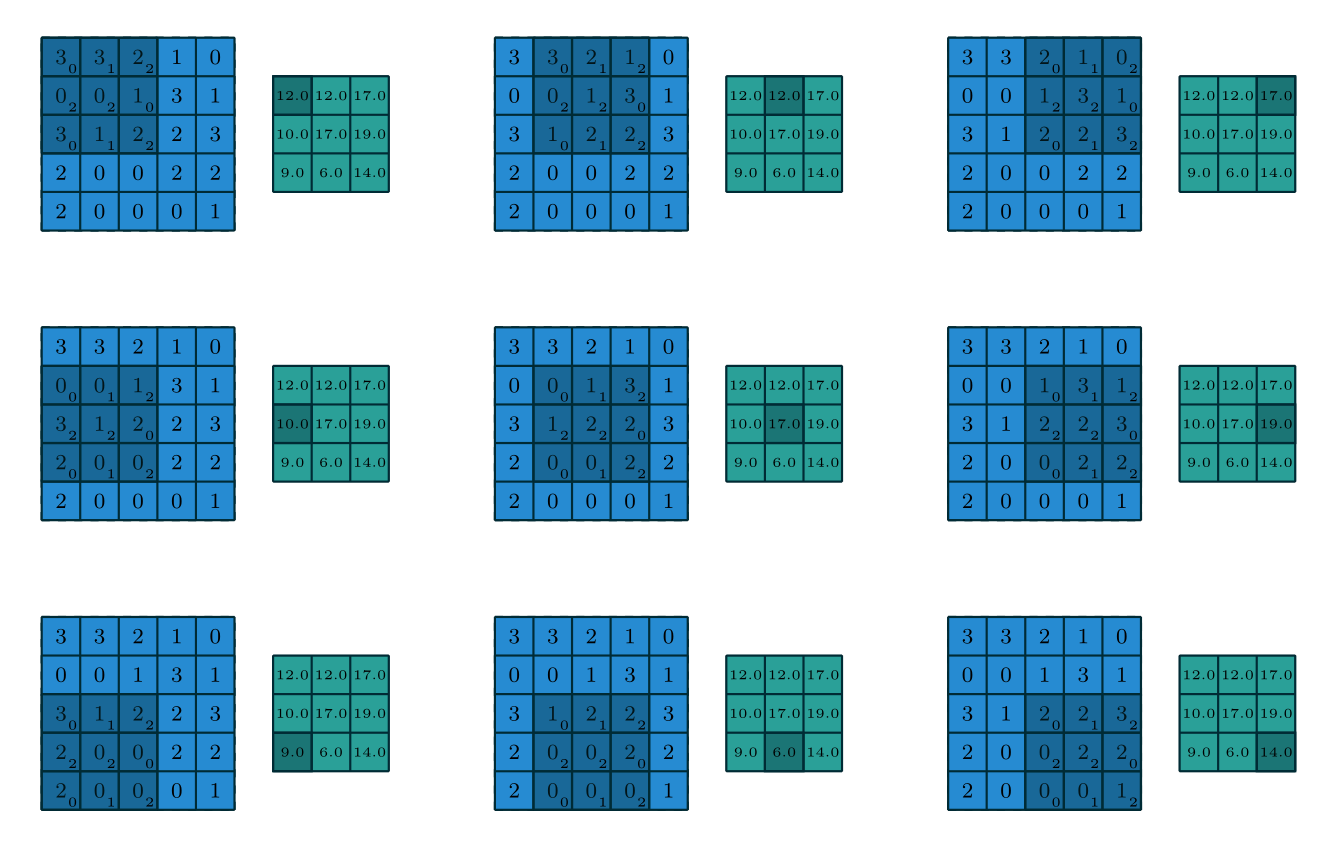
\includegraphics[width = 1.0\textwidth]{./Figures/1603_07285v1_convolving.PNG} %convolving
		\rule{35em}{0.5pt}
	\caption[Convolution]{Activations from layer 1 (shown as the blue grid) are convolved with the kernel (shown by subscript values in the convolution window) to produce a weighted sum for every neuron in the layer above (shown by the green grid). As the kernel size is $3\times 3$, a convolution with a single block stride to all sides will produce a $3\times 3$ grid. This can be altered by padding grid with zeros.}
	\label{fig:Convolution}
\end{figure}

\subsubsection{Pooling}
Following convolution \textit{pooling} is applied.
The role of pooling is to merge semantically similar features into one.
For example, the relative positions of the features forming a alphabetic letter can vary.
A way to reliably detect the feature can be done by coarse-graining (reducing the spacial resolution of) the position of each feature in a manner that preserves relevant information whilst removing sensitivity to noise, translations and distortions\citep{dengthree}\citep{lecun1995convolutional}\citep{bengio2009advances}.

The pooling layer subdivides the convolution layer output into regions of size $z \times z$ known as \textit{pooling windows}\citep{chen2014big}. 
Each window is reduced to a single value with the \textit{pooling function}, see Figure ~\ref{fig:Pooling}.
Pooling windows may be over-lapping but this has empirically been shown increase over-fitting\citep{bengio2009advances}\citep{krizhevsky2012imagenet}.

\begin{figure}[htbp]
	\centering
		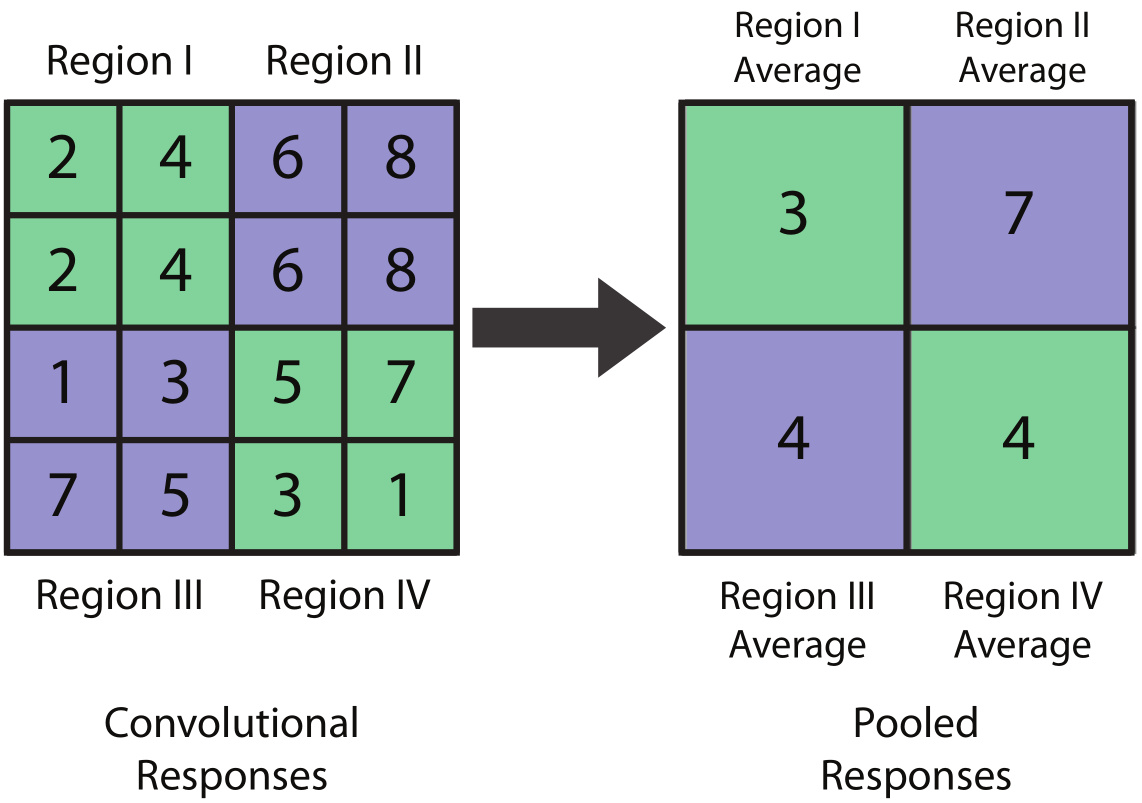
\includegraphics[width = 0.6\textwidth]{./Figures/convolution_end_to_end_recognition_with_cnns.jpg} %Pooling
		\rule{35em}{0.5pt}
	\caption[Pooling]{Convolution responses are pooled with an averaging function using non-overlapping windows.}
	\label{fig:Pooling}
\end{figure}

The net effect of weight sharing in the convolutional layer followed by a pooling scheme provides the CNN with natural translation in-variance properties\citep{dengthree}, see Figure ~\ref{fig:CNN}.
The pooling function is usually \textit{xax-out}.
This is the maximum, $max(f_i)$, where $f_i$ refers to all elements in the pooling window\citep{bengio2009advances}\citep{lecun2010convolutional}.

Maxout serves two purposes:
\begin{enumerate}
\item It picks out the highest activation in a local region, thereby providing a small degree of spatial invariance.
\item It reduces the number of activations for the next layer by a factor of $z^2$.
With a smaller feature-map less parameters to be learnt in the later layers.
\end{enumerate}

Alternatively, the pooling function may be the average, $\sum_i(f_i)/z^2$, as in Figure ~\ref{fig:Pooling}.
Typically pooling window size and stride are hand-designed, however algorithms exist which generate learn-able pooling regions\citep{bengio2009advances}\citep{lecun2015deep}.
\begin{figure}[htbp]
	\centering
		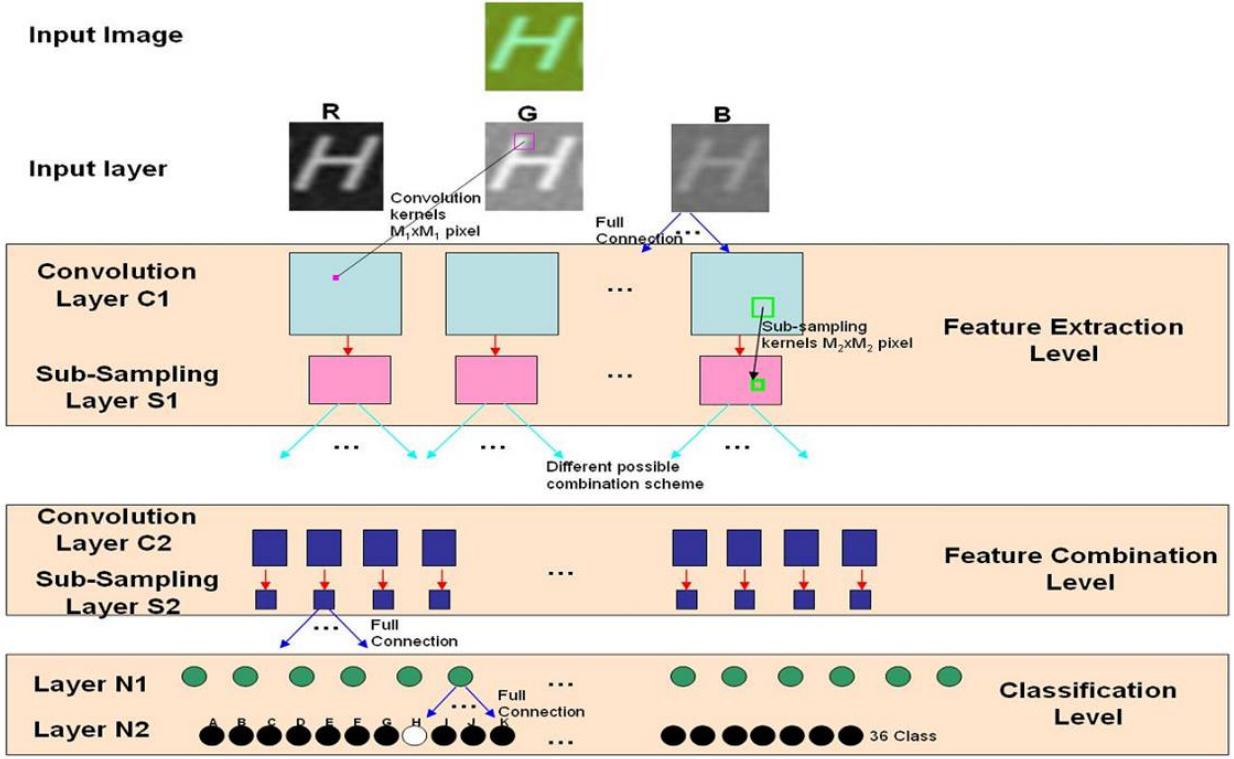
\includegraphics[width = 1.0\textwidth]{./Figures/CNN_network_sparse_coral_classification_3.jpg} %CNN Structure
		\rule{35em}{0.5pt}
	\caption[CNN Architecture]{A standard image will have three layers of intensity values for the red, green and blue pixels respectively. A stacked tensor of RGB values can be convolved with a 3D kernel or, as in the case above, each layer is convolved with a 2D kernel separately. All produced feature-maps are subsequently sub-sampled with pooling. CNN architectures may vary in may ways such as kernel shape, pooling window size, pooling functions and number of layers. After several stages there are many small feature maps. Commonly they are connected to an MLP used for classification or regression tasks.}
	\label{fig:CNN}
\end{figure}

As all kernel weights are learned via back-propagation CNNs can be understood to be synthesizing their own feature generators\citep{lecun1995convolutional}.

\begin{figure}[htbp]
	\centering
		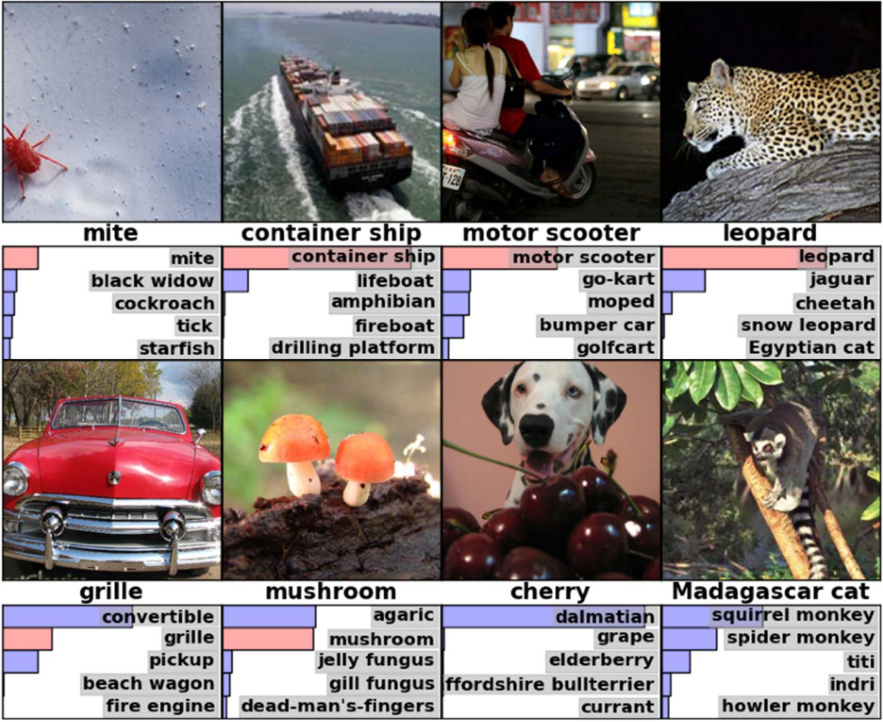
\includegraphics[width = 0.8\textwidth]{./Figures/CNN_image_prediction_krizehevvsky_nips_2012.jpg} %IMAGENET example
		\rule{35em}{0.5pt}
	\caption[Image Recognition]{A CNN was trained as part of the Imagenet Recognition Challenge\citep{deng2012imagenet}. The dataset was composed of approximately 1000 images for each of 1000 categories. Shown above are the top 5 predictions for each of the test images. The model achieves a top-1 and top-5 error rate of $37.5\%$ and $17.0\%$ respectively. A top-5 error rate is the fraction of test-objects not seen in the top five model predictions. Even where the top-1 is wrong the top-5 predictions seem reasonable. In fact, on the bottom row the model appears to be more accurate than the provided labels.}
	\label{fig:Image_predication}
\end{figure}

\section{Measuring Performance}
Two primary sources of data exist when producing a model, a training and test set.
The training data is used to tune the model parameters; the model learns from training data.
However, in order to produce an independent measure of the model's performance a test set must be used.
It may be quite intuitive to think a model's success can be completely measured by the accuracy of predictions on the test set, however this does not tell the whole story.
%Accuracy
%Motivation for Precision Recall F-measure 
%Confusion Matrix
%AUC.
%Critical Evaluation

\subsection{Test Performance Error}
If we measure a model to have an accuracy of $85\%$ this does not tell us how much the true value may differ with different degrees of confidence.
We would be more confident of the accuracy being near the $85\%$ if we got that result from a test set of 10,000 instances than of 100.
We consider the test to be like a Bernoulli process in order to give some measure of confidence.
In statistics, a Bernoulli process is one in which a succession of independent events can have one of two results, like pass or fail, correct or not.

This has a simple method for providing confidence intervals\citep{witten2005data}.
\be
p \pm z \sqrt{\frac{1}{n} p(1 - p)}
\ee
where $p$ is the accuracy estimated from the test set, $z$ is the $1 - \frac{1}{2}\alpha$ quantile often given in the back of many statistical textbooks, and $n$ is the number of samples within the test set.

\subsection{Confusion Matrix} 
If $80\%$ of the test set are dogs, and $20\%$ are not, then a model can get an accuracy of $80\%$ just by guessing `dog' every time; clearly not a very useful model.
This motivates the use of a \textit{Confusion Matrix}.
A confusion matrix is a table counting the occurrences of all the possible model prediction outcomes.
For every classification there are four possible outcomes.
If the model correctly predicts `dog', it is called a true positive (TP); if incorrectly classed as `not a dog' then it is a false negative (FN).
On the other hand, if the model correctly predicts the object to \textit{not} be a dog it is a true negative (TN); but if classified as dog when it is not, then it is a false positive (FP).

We can construct a confusion matrix, also called a \textit{contingency table}, counting all the outcome types from the test set.
Each row in the table refers to the true classes and each column classifier predictions\citep{flach2012machine}, see Figure ~\ref{fig:Confusion_matrix_2}.
\begin{figure}[htbp]
	\centering
		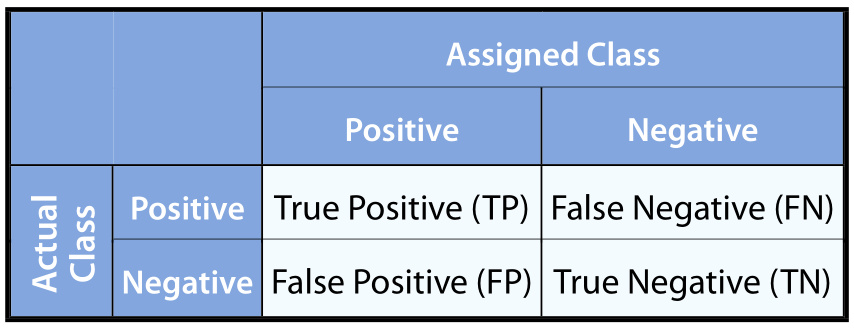
\includegraphics[width = 0.8\textwidth]{./Figures/encyplopedia_of_machine_learning_confusion_matrix.jpg}
		\rule{35em}{0.5pt}
	\caption[Confusion Matrix]{A confusion matrix encapsulates the success of a binary classification model. Ideally all true positive classes will be labelled as positive, \textit{True Positives}; and all negative classes as labelled as negative, \textit{True Negatives}. These will only fill in the tables backward diagonal. The forward diagonal shows cases in which the prediction was incorrect. If predicted positive where truly negative a \textit{False Positive} is committed. Alternatively when predicted negative but truly positive, a \textit{False Negative} has been committed.}
	\label{fig:Confusion_matrix_2}
\end{figure}

From the confusion matrix we can calculate a range of performance metrics.
Accuracy is the simplest
\be
Accuracy = \frac{TP + TN}{TP + TN + FP + FN}
\ee
that is the sum of the correct predictions over the total.

\subsection{Precision and Recall}

Two other useful measures of performance are \textit{precision} and \textit{recall}\citep{flach2012machine}\citep{ball2010data}.
Recall - also known as \textit{Completeness}, \textit{Sensitivity} or \textit{True Positive Rate} (TPR) - is the fraction of objects truly belonging to a category that are correctly classified as such,
\be
Recall = Completeness = Sensitivity = TPR = \frac{TP}{TP + FN} 
\ee

The False Positive Rate(FPR), or `Type 1 error', is the fraction of positive classifications which are incorrect given by
\be
FPR = \frac{FP}{FP + TN}
\ee
which relates to the \textit{Specificity}, or fraction of the negative class correctly classified,
\be
Specificity = \frac{TN}{FP + TN} = 1 - FPR
\ee
\textit{Precision} (also known as \textit{Efficiency}) is the fraction of objects classified as a class that truly belong to that class:
\be
Efficiency = Precision = \frac{TP}{TP + FP} 
\ee

The ideal would be to have both precision and recall to be close to one, however there is often a trade-off between the two.
The preferred balance between precision and recall will be problem-dependent and may hinge on not having too much contamination of the positive class, or the economic costs of incorrect classifications.

In practice Precision and Recall are particularly important measures in the case of \textit{skewed classes}.
Skewed Classes is the scenario in which one class significantly outnumbers the other class or classes in a data set.
For example when detecting fraudulent behaviour in on-line banking, the majority of activity will be normal.
Should a classifier predict the activity is normal all the time (clearly a bad classifier) it will still be right most of the time and score a high accuracy.

\subsection{F-measure}
A measure that combines precision and recall to give an indication of the algorithm's success is the $F_\beta$ measure (for real non-negative values of $\beta$)\citep{sokolova2006beyond}\citep{davis2006relationship}:
\be
F_\beta = \left(1 + \beta^2\right)\frac{precision.recall}{\beta^2.precision + recall}
\ee
The F-score favours Precision when $\beta > 1$, is evenly balanced when $\beta = 1$ and favours Recall where $\beta < 1$.
When balanced we have the \textit{F-measure} or\textit{ balanced F-score},
\be
F_1 = 2\frac{precision.recall}{precision + recall}
\ee
which ranges from zero to one.

\subsection{ROC Curve and AUC Score}
The Receiver Operating Characteristic (ROC) curve is an encompassing visualization of a binary classifier's performance\citep{sokolova2006beyond}\citep{davis2006relationship}\citep{fawcett2006introduction}.
They have long been used in signal detection theory as a way of visualizing and evaluating the trade off between false alarms and correct hits and are commonly used in the design of medical diagnostic tests which are not $100\%$ accurate.
ROC curves are useful because they allow for better analysis of the trade-off between the false positive rate and the true positive rate.

Consider a case of two classes.
Formally each example $E$ is mapped to one of the set $\{p, n\}$ which are positive and negative labels respectively.
The classier or model is a mapping from each example to one of the classes.
Some models will do this by producing continuous output, often a number between $0$ and $1$, to which thresholding is applied.
If the output surpasses the threshold it is classified as $1$, for positive, otherwise $0$ for negative.

The ROC curve is a plot of TPR on the Y-axis vs FPR on the X-axis.
For a model that produces continuous output, by changing the threshold you can obtain many pairs of $(TPR, FPR)$ values which on a scatter-plot produce an \textit{ROC curve}, see Figure ~\ref{fig:ROC_curve_2}.
For a model that has discrete output, even before any threshold, this will only be a single point on the graph corresponding to the only $(TPR, FPR)$ pair.
Such discrete scoring classifiers can often have their internal state converted into a score rather than a discrete outcome which will provide a full ROC curve.
An example of this is in the decision tree algorithm that produces its discrete output based on the proportion of one instance over another at the final node.
By just using the ratio, and not choosing the most common label you have a continuous score.
\begin{figure}[htbp]
	\centering
		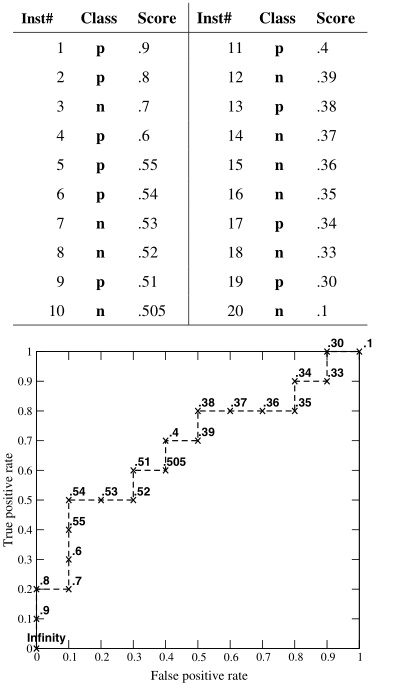
\includegraphics[width = 0.7\textwidth]{./Figures/ROC_curve.jpg}
		\rule{35em}{0.5pt}
	\caption[The ROC Curve]{A classification model that produces continuous output can vary in performance based on the threshold chosen. To provide an unambiguous measure a Receiver Operating Characteristic (ROC) Curve is used. In the example above continuous scores have been assigned to each of the 20 instances where their true class is known. The curve is made by plotting the True Positive Rate (TPR) vs the False Positive Rate (FPR) for all possible threshold values (shown above the crosses). The final threshold selected is problem-dependent. In general terms a model with ROC curve that hugs the $(0,1)$ point is preferred.}
	\label{fig:ROC_curve_2}
\end{figure}

The ideal model should go through the point $(0, 1)$, that is where there are no false positives and a $100\%$ true positive rate.
Classifiers that appear toward the left hand side of the plot can be thought of as conservative, in that they require strong evidence to make a positive classification.
However, their stringent criteria will make few examples classified as positive.
Classifiers appearing toward the upper right are quick to label an example as positive, so they are likely not to miss positive classifications.
Their lax criteria will likely contaminate the pool of positives with many incorrectly labelled negatives.
As there are generally more negative cases than positive, more non-cats then cats, behaviour of the ROC curve toward the upper left tends to be the most informative.

If a models ROC curve lies along the 45 degree $y = x$ line it means the classifier is either randomly guessing, or it has not learned a useful data representation.
For example ,if it guesses positive half of the time it will have a TPR equal to $0.5$, however as now half of the negatives will be incorrectly classified the FPR will equal $0.5$ as well.
This $TPR = FPR$ trend will be true for any percentage of a random example being positive, yielding a line along $y = x$.
In fact, if the proportion of positive to negative classes changes an ROC curve will not be affected at all.
This insensitivity to skew classes is what makes ROC curves so useful.
Classes that outnumber their opposite class are very common in real world problems making a performance measure invariant to skewness even more valuable.
In some cases the skewness of classes may alter with time, such as the number of infected people over time, but that should not change the fundamental characteristics of what identifies someone as infected by a disease.
Should a model appear below the $y = x$ line this means it performs even worse than random guessing.
This is not necessarily a bad thing as the model has captured a useful data representation but is making incorrect conclusions.
Should label predictions be swapped around, positive to negative and vice versa, the model performance is improved.

It will often be the case that the most natural threshold of $0.5$, for a model output between $0$ and $1$, is not the best.
Depending on the model and the problem it may be that selecting the threshold to be $0.6$ has a better TPR without increasing the FPR.

A common way of comparing models to each other in a single measure is to use the \textit{Area Under an ROC Curve} (AUC), see Figure ~\ref{fig:AUC_score}.
A perfect classifier would reach a TPR of 1 and FPR of 0, so the curve would be a straight line along $TPR = 1$ with an area underneath of 1.
A classifier that performs no better than random, a line of $y = x$, would score half of the total area, $0.5$.
It is still possible for a model with a lower AUC score to perform better than a model of higher AUC score in a particular domain.
Therefore, one should not necessarily select the model with the highest AUC score as it depends on the costs of true positives and a false negatives.
For example, if astronomers make a classifier of abnormal galaxies in order to follow them up with further study, it is more important to have a high TPR, even at the risk of weeding out some abnormal galaxies, than it is to have a low TPR but high FPR.
If there are a large number of false positives the data set is essentially contaminated with a large pool of galaxies the astronomers cannot afford telescope time to waste on.
Here fewer positives of high quality is better than many positives of low quality.
So if a model happens to perform best in the ROC region of interest even though it has lower AUC score it would be the `economical' choice.
\begin{figure}[htbp]
	\centering
		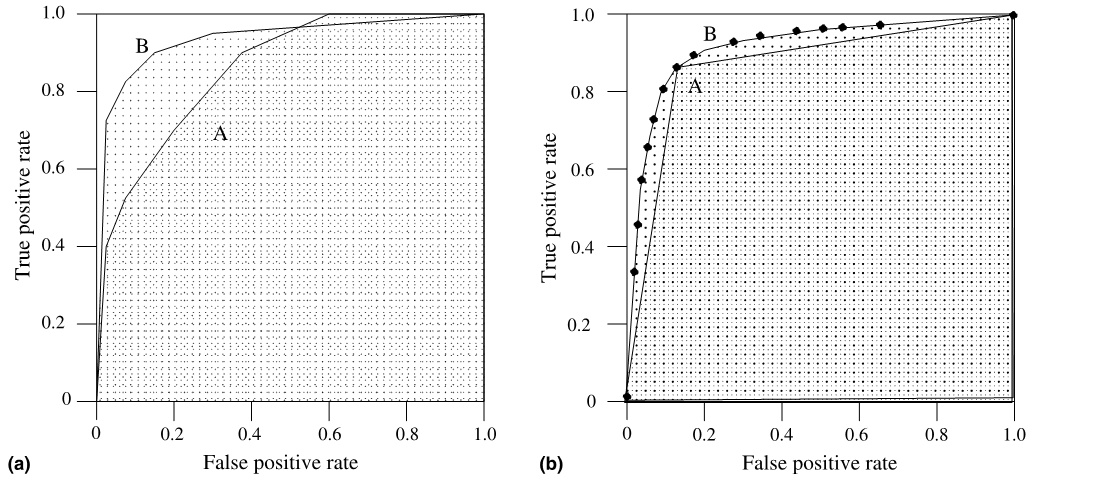
\includegraphics[width = 1.0\textwidth]{./Figures/AUC_measure_introduction_to_roc_analysis_2.jpg}
		\rule{35em}{0.5pt}
	\caption[The AUC Score]{The Area Under Curve (AUC) score is the area under the ROC curve. A perfect model will have an area of 1 $unit^2$. This measure is better for evaluating the general performance of one model vs another when the model with higher TPR may vary depending on the FPR domain.}
	\label{fig:AUC_score}
\end{figure}

Selecting the model with the highest AUC score suffers from the same problem as picking a model of higher accuracy.
Without a measure of the variance this score can only be trusted so much.
This can be done by testing on multiple test sets generated via cross-validation and then averaging.

\section{SDSS Survey}
This section supplies the necessary knowledge of supernovae for this thesis.
Following this machine learning as a tool for handling astronomy data is discussed.
Thereafter, we discuss the Sloan Digital Sky Survey (SDSS), the objectives, data and current methodology for data handling.
As a potential solution to data handling problems of modern astronomy this thesis proposes the use of deep learning techniques as superior to the more classical machine learning methods.
In this light we discuss results for prior work on the application of machine learning to supernovae detection.
%Supernovae
%Transient Types

%The LDSS Survey
%Data origin

%Difference Imaging
%State of other research
%Critical Evaluation

%Data Specs
%Fakes
%Specto Confirmed
%Data Splitting
\subsection{Supernovae}
A supernova (SN), illustrated in Figure ~\ref{fig:supernovae}, is a powerful explosive event at the end of a stars lifetime\citep{du2014machine}.
In fact so much energy is released that the star briefly outshines the host galaxy\citep{baade1938photographic}.
Different supernovae (SNe) types may be classified by their spectral features.
Type I SNe have no hydrogen lines, unlike Type II SNe which do.
Type 1 may be broken up into a three subtypes: Type Ia have strong signatures of higher-mass elements such as silicon, sulphur, iron and calcium but little of hydrogen and helium; Type Ib have prominent helium lines and Type Ic have neither hydrogen nor helium.
The features arise from differences in the explosion source.
Type Ia are the result of the thermonuclear explosion of a white dwarf, which is the last stage of many stars' lifetimes where the envelope of gases has been expelled to reveal a degenerate core - extremely dense matter that is supported from collapsing in on itself by the Pauli exclusion principle.
%Add reference
The other types, Ib, Ic and II, are the result of a star's core collapsing in on itself.
\begin{figure}[htbp]
	\centering
		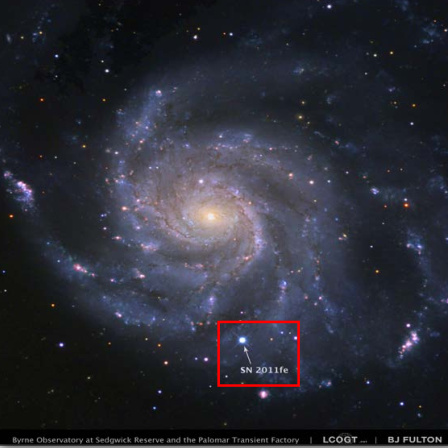
\includegraphics[width = 0.8\textwidth]{./Figures/encyplopedia_of_machine_learning_SN.jpg}
		\rule{35em}{0.5pt}
	\caption[Supernovae]{An image captured by the Palomar Transient Factory of the Pinwheel Galaxy (M101) shows a single exploding star (framed in red), a \textit{supernova}, which can outshine an entire galaxy.}
	\label{fig:supernovae}
\end{figure}
\begin{figure}[htbp]
	\centering
		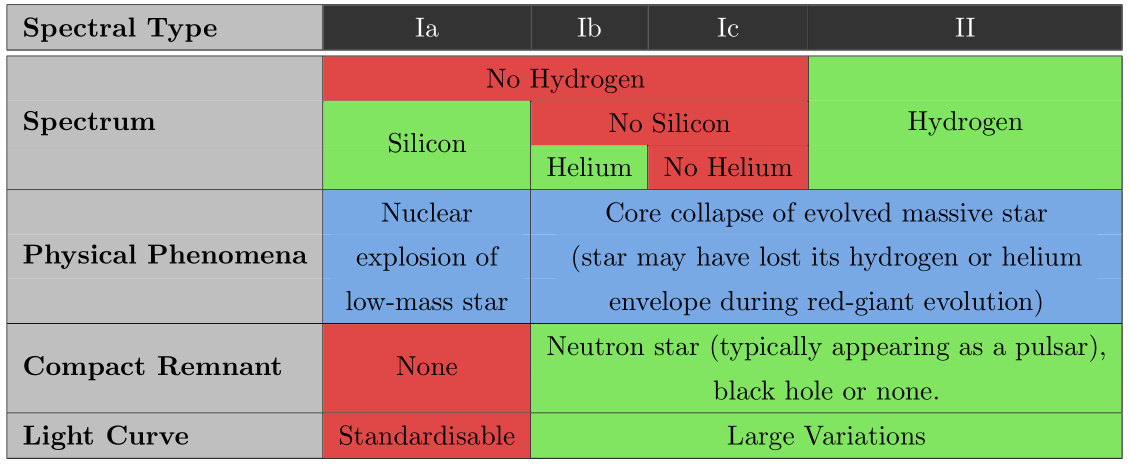
\includegraphics[width = 0.8\textwidth]{./Figures/lise_thesis_SDSS.jpg}
		\rule{35em}{0.5pt}
	\caption[Supernovae Types]{There are several classes of SNe. Type Ia originate from the nuclear explosion of a low mass star and has consistent light curves. Their spectra have no hydrogen but contain silicon. Type Ib has helium unlike Ic, but both lack hydrogen and silicon. Type II is the only type with hydrogen. Type Ib, Ic and II all originate from core collapse of a massive star and vary greatly in light curve features.}
	\label{fig:supernovae_types}
\end{figure}

A Type Ia occurs in binary systems where two stars, a white dwarf and a larger companion star, orbit one another.
If the companion star enters its red giant phase 1 it starts to inflate to a point where some matter can no longer be bound.
The free matter leaking off the red giant is then slowly accreted by the white dwarf.
The white dwarf's mass will increase, but it cannot do so indefinitely as the nuclear forces preventing collapse can only handle so much.
Once the Chandrasekhar limit ($1.4M_{\odot}$, where $M_{\odot}$ denotes solar mass) is reached the core collapses resulting in a thermonuclear explosion which destroys the star within seconds leaving an expanding gaseous remnant rich in metals.
The remaining supernovae types occur when a massive star ($M > 9M_{\odot}$) can no longer withstand its own gravitational pressure and collapses.
The imploded core can remain either as a neutron star (usually in the form of a pulsar) or collapse further into a black hole, or it can be entirely destroyed.
Supernovae differ not only in spectra but light curves too.
A light curve is a plot of a supernova's intensity over time.
The light curves of types Ib, Ic and II SNe can vary substantially depending on the progenitor's metallicity and mass, as shown in Figure ~\ref{fig:supernovae_curve_types}.
As a Type 1a occurs when a white dwarf accretes exactly the right mass their light curves are typically brighter and have very similar light curves.
\begin{figure}[htbp]
	\centering
		\includegraphics[width = 0.9\textwidth]{./Figures/lise_thesis_light_curves_of_SN.PNG}
		\rule{35em}{0.5pt}
	\caption[Supernovae Light Curves]{Star mass, metallicity and other factors cause SNe to have different light curves. Even within different SNe types there is variation with the exception of Type Ia. }
	\label{fig:supernovae_curve_types}
\end{figure}
It is for this reason that Type Ia SNe are particularly useful for cosmologists to measure distance.
The further away the SN the dimmer it will appear.
In addition, the obtained spectra will be appropriately red-shifted in accordance with their recession from us due to the expansion of the universe.
If one knows how bight a candle burns and how dim it appears one can tell how far away the candle is.
Type Ia light curves and spectra allow for exactly this on a cosmological scale, making them `standard candles', see Figure ~\ref{fig:light_curves}.
In this manner the accelerating expansion of the universe was discovered\citep{riess1998observational}\citep{perlmutter1999measurements} which has since motivated even larger supernovae surveys.
\begin{figure}[htbp]
	\centering
		\includegraphics[width = 1.0\textwidth]{./Figures/lise_paper_light_curves.jpg}
		\rule{35em}{0.5pt}
	\caption[SNe Ia Light Curves]{A Supernova event can be seen for weeks. A time-series of the light intensity is known as a \textit{light curve}. For Type Ia, the trigger conditions are so similar as to produce nearly the same light curves viewed at the same distance. As they are equivalently as bright as one another the change in flux, and Doppler shifted light-curves can be used to infer their distance; making them very useful \textit{standard candles}\citep{branch1992type} in cosmology. }
	\label{fig:light_curves}
\end{figure}

\subsection{The SDSS Survey}
%What is the SDSS
The Sloan Digital Sky Survey (SDSS-II) is a multi-spectrum spectroscopic red-shift survey run during three-month campaigns in the Fall of 2005, 2006, and 2007 as part of the extension of SDSS-I.
The SDSS-II SNe Survey was commissioned to address the following goals\citep{abazajian2009seventh}:
\begin{enumerate}
\item Refine the SNe Type Ia Hubble diagram.
At the time the Hubble diagram  was constructed from low - $(z \approx 0.1)$ and high-red-shift $(z \approx 0.3)$ Type Ia samples from multiple telescopes of differing passbands and selection criteria, introducing systematic errors.
The SDSS-II SNe Survey would gather distance estimates for Type Ia SNe in the sparsely populated red-shift range $0.05 < z < 0.35$ to better constrain the Hubble parameter.
\item Minimise SNe systematics.
At the time most SNe surveys had systematic errors comparable to their statistical errors.
Systematic errors in the SDSS-II SNe Survey would be significantly reduced.
Photometric calibration errors of $1\%$ in Stripe 82 were achieved from the many years on the large-scale calibration of the data during SDSS-I.
In addition, the spectroscopic filters had well measured transmission curves and were all situated on the same stable camera.
\item Fix rest-frame ultraviolet light curves.
SNe at red-shift $z > 1$ have their light curves matched to templates of the rest-frame light curve to reduce systematic errors.
For example the 3600 \AA (the u-band) in the SN rest-frame corresponds to $ \approx 8000$ \AA at a red-shift of $1.2$.
At very far red-shift, $z = 0.3$, the SDSS would be capable of observing this region at $4700$ \AA, the g-band.
The measurements can then be used to improve template data in the rest-frame ultraviolet region.
\item Explore photometric methods to measure SNe characteristics.
Spectra measurements of candidates are a luxury available only when other telescopes have free time and favourable conditions.
The SDSS large depository of photometric data would allow a search for a more practical photometric method of SNe classification and red-shift determination.
\item Study SNe types, rates and host galaxies.
SNe rates of occurrence per galaxy could be estimated for the different SNe types.
In addition, the SNe host galaxies identified could be studied for information about progenitor properties.
\item Finally, SDSS-II would serve as a probe for rare and interesting objects as yet unknown to astronomy.
\end{enumerate}

%Operation
The SDSS 2.5 m telescope and imaging camera are located at the Apache Point Observatory in New Mexico which produces photometric measurements in each of the $u$, $g$, $r$, $i$ and $z$ spectrum filters spanning wavelengths 350 to 1000 nm.
SNe are difficult to detect in the $u$ and $z$ filters except at low red-shifts ($z \approx 0.1$ for Type Ia) due to the relatively poor filter throughput.
Beyond a red-shift of 0.4, Type Ia can still be detected, but after $z \approx 0.2$ the ability to obtain high-photometry quality deteriorates quickly.
During the survey the camera is operated under a ``rolling search''.
This is where a portion of the sky is repeatedly scanned to discover new SNe and measure their respective light curves in the intermediate red-shift range of $0.05 < z < 0.35$.

%Camera 
The SDSS telescope camera, illustrated in Figure ~\ref{fig:sdss_camera}, is comprised of six sensor columns each of which contains five CCD chips corresponding to the $r$, $i$, $u$, $z$ and $g$ filters, see Figure ~\ref{fig:band_efficiencies} for corresponding frequency sensitivities.
The telescope is oriented such that a patch of sky drifts through the cameras field of view; known as \textit{drift-scanning}.
The focused image will drift across the columns providing 55 seconds worth of exposure to each CCD.
Sensor readings for a single point in the sky cannot be taken simultaneously as not all CCD’s are exposed to that point.
Instead CCD’s are read out in sync with the drifting i.e. 55 seconds apart.
Such drift scanning allows the telescope to image long continuous strips of the sky.
\begin{figure}[htbp]
	\centering
		\includegraphics[width = 0.8\textwidth]{./Figures/lise_paper_sdss_camera.jpg}
		\rule{35em}{0.5pt}
	\caption[SDSS Camera]{The SDSS photometric camera has five CCD chips for each of the $riugz$ bands in each of six sensor columns. The camera is oriented such that by the natural rotation of the sky the point of exposure drifts down over the column, taking 55s to cross over each of the rows. }
	\label{fig:sdss_camera}
\end{figure}
\begin{figure}[htbp]
	\centering
		\includegraphics[width = 0.8\textwidth]{./Figures/SDSS_EDR_band_effieciency.jpg}
		\rule{35em}{0.5pt}
	\caption[Response Curve]{The upper curves are the quantum efficiencies for light absorption for each of the $ugriz$ filters ignoring atmospheric effects. The lower curve includes the atmospheric effects assuming an air mass - the optical path length through Earth's atmosphere - of 1.3. Further scattering within the chips affects only the $r$ and $i$ bands with the corresponding response curve given by the dashed lines.}
	\label{fig:band_efficiencies}
\end{figure}

%Location
Exposure time per unit area limits the survey from operating over the whole sky.
Instead only Stripe 82, shown in Figure ~\ref{fig:sky_coverage}, was observed.
This is a 300 $deg^2$ area along the celestial equator, 2.5 deg wide in Declination and between Right Ascension of 20 h and 04 h.
It takes about two nights to cover all of Stripe 82 in this way.
However, the average \textit{cadence}(frequency of observation) was approximately four nights as a result of bad weather conditions and interference from moonlight.
Stripe 82 was used to take advantage of the already extensive object databases, reference images and photometric calibration created by SDSS-I.
As both surveys used the same telescope for photometrics this minimised systematic errors that may occur from differing photometric standards on different telescopes.
\begin{figure}[htbp]
	\centering
		\includegraphics[width = 0.7\textwidth]{./Figures/SDSS_EDR_sky_coverage.jpg}
		\rule{35em}{0.5pt}
	\caption[SDSS Coverage]{The SDSS survey is limited in the area of the sky that it can scan by both being ground-based and requiring long exposure times. Shown above is Stripe 82 which was scanned roughly every four nights.}
	\label{fig:sky_coverage}
\end{figure}

%Difference Imaging
SDSS imaging software\citep{stoughton2002sloan} was used to process the raw images and SNe were identified via a frame subtraction technique\citep{alard1998method}).
Each picture of the sky, the \textit{Search Image}, would be subtracted from the most recent previous image of the sky, the \textit{reference image} in the same position, see Figure ~\ref{fig:transient_detection}, resulting in a \textit{Difference Image}.
This was only done in real-time using the $g$, $r$ and $i$ bands, as they are most useful for SNe detection.
Using just 3 bands allows for more easily interpretable false-colour RGB image to be made.
Unless a transient occurred, this will leave a pure noise image.
The SNe candidates would then be filtered by an automated object detection algorithm requiring that difference images have a noticeable difference detected in two or more filters, not coincide with existing catalogued stars or variable objects, and were not seen to be moving during the $r$ and $g$ band exposures.
In 2006 and 2007, further software cuts were made to lessen the number of images for hand scanning.
The change significantly reduced the number of moving objects, diffraction spikes, and long-term variable objects by cross-matching with a veto catalogue.
Now, single-epoch detections would be sent on-wards to manual scanners if they were not moving, bright enough ($M_r < 21$ or $M_g < 21$) and detected in at least two epochs.
\begin{figure}[htbp]
	\centering
		\includegraphics[width = 1.0\textwidth]{./Figures/Transient_detection_The_difference_imaging_pipeline_for_the_transient_search.jpg}
		\rule{35em}{0.5pt}
	\caption[Transient Classification]{A difference images is produced by subtracting a new image from a reference image. Should a peak with large signal to noise ratio be detected it is a transient. Shown above is the difference image for the $i$-band in deep field C3 on 13 October 2013. Noted transients are outlined (in red) below. Outlined in dashed red-boxes are objects that failed initial detection cuts. Objects in solid red boxes passed the cuts but were then ruled out by an \textit{autoScan} algorithm. The objects outlined in yellow circles path both tests and are potential SNe candidates.}
	\label{fig:transient_detection}
\end{figure}

%Detection
In the past, removal of false detections was done manually by astronomers, see Figure ~\ref{fig:hand_scanning} for the decision-tree.
During hand scanning, obvious artefacts such as in Figure ~\ref{fig:transient_examples} were removed.
Artefacts can be produced via diffraction spikes, CCD saturation, bleeding and registration errors among others.
However, this hand-scanning process was imperfect and led to a large number of artefacts that constituted $70\%$ or more of the candidates.
A team of roughly twenty hand scanners used the $g$, $r$ and $i$-band search and difference images (each having a size of $51 \times 51$ pixels) and object history to classify each of the candidate objects into one of ten possible classes: dipoles, artefacts, saturated stars, transients, variables, moving objects, SN Gold, SN Silver, SN Bronze and SN Other\citep{frieman2007sloan}.
For SDSS-II supernova survey, this meant hundreds or thousands of images being manually scanned each night.
Unfortunately it has been found that classification is done inconsistently between people or even the same person over time depending on mood and exhaustion.
\begin{figure}[htbp]
	\centering
		\includegraphics[width = 0.9\textwidth]{./Figures/lise_paper_hand_scanning.jpg}
		\rule{35em}{0.5pt}
	\caption[Hand-scanning]{Hand-scanners labelled the transients in the dataset according to the decision tree above.}
	\label{fig:hand_scanning}
\end{figure}

Even if the transient is genuine it may not be a SN but an asteroid, variable star, cosmic ray or artificial satellite, see Figure ~\ref{fig:transient_examples} for some examples.
\begin{figure}[htbp]
	\centering
		\includegraphics[width = 1.0\textwidth]{./Figures/transient_examples_Real-time_detection_of_transients_in.jpg}
		\rule{35em}{0.5pt}
	\caption[Artefacts]{Many apparent transients are imaging artefacts or are not supernovae. Each of the difference images above show artefacts and their source of occurrence.}
	\label{fig:transient_examples}
\end{figure}

Figure ~\ref{fig:transient_types} shows a summary of the many different genuine transients.
Should other telecopes be available they can be used to validate the remaining SNe candidates\citep{adelman2008sixth}.
\begin{figure}[htbp]
	\centering
		\includegraphics[width = 1.0\textwidth]{./Figures/Transient_types_Thirty_metre_deatiled_science_case.jpg}
		\rule{35em}{0.5pt}
	\caption[Transient Variability]{The variability tree summarizes the potential sources of detected transients.}
	\label{fig:transient_types}
\end{figure}

As hand-scanning accuracy is paramount, fake SNe were injected into the pipeline to provide quality control and calculate the average detection efficiency per human\citep{kessler2015difference}\citep{dilday2008measurement}.

%Research Motivation
Regardless of human accuracy, eye-scanning of future sky surveys such as the Large Synoptic Survey Telescope (LSST) will not be possible due to the millions of detections per night.
The LSST is expected to find 1,000 new supernovae each night for 10 years; at least a million Type Ia SNe over its lifetime, effectively generating one SDSS each night\citep{abell2009lsst}\citep{mickaelian2015astronomical}.
Such Big Data demands new statistical inference and machine learning techniques for processing and analysis.
This concern is what motivates this dissertation on applying Deep Learning techniques to the detection of SNe.

%Data Specs
Throughout the SDSS-II SNe Survey 10,258 new variable objects were discovered and 500 Type Ia were spectroscopically identified including 81 core-collapse SNe.
The final data release was of all transient sources brighter than $\approx 22.5$ mag that had no known variability prior to 2004 and excludes known active galaxies.
The obtained full data-set contains 27,480 objects of which 11,959 are not-real and 15,521 are real.
Data from 2005 were omitted because of the different threshold cuts employed at the time so as not to introduce unnecessary variation into the data-set.
For classification purposes, the original classes were regrouped into three new visual classes, ``artefacts'', ``real objects'' and ``dipoles/saturated''.
Residuals of real objects are point-like (convolved with the telescope and atmosphere’s seeing), artefact residuals resemble diffraction spikes and dipoles/saturated objects are often quite point-like, typically with negative flux in some part of the image stemming from saturated CCD effects or registration errors.

\subsection{Previous Results}
%Prior Research
Prior work on automatic classification has been done as part of the SNe factory where difference image attributes such as position, shape, Full Width Half Maximum (FWHM) and distance to the nearest object in the reference image are used to discriminate between fakes and transients\citep{bailey2007find}\citep{romano2006supernova}.

Recently several `classical' machine learning algorithms to the classification of candidate SNe\citep{du2014machine}.
These include Naive Bayes(NB), Support Vector Machines(SVM), K-Nearest Neighbours(KNN), a three layer MLP(using the python SkyNet package), Minimum-Error Classification(MEC) and Random Forests(RF).
The features used in all these algorithms were derived with several data-reductions methods.
Principal Components Analysis(PCA)\citep{jolliffe2002principal} performs an orthogonal rotation in the complete feature space such that the first axis of the new set of co-ordinates, or the first principle component, is oriented in the direction of greatest variance.
The second PCA component direction will have less variance and so on.
In doing so this also removes any linear correlation between PCA components.
Each sample in the dataset can be entirely described by using the $N$ PCA co-ordinates instead of the original $N$ features.
However, the reducing variance of the PCA components means that earlier PCA components likely carry more information.
If only the first $M$ components are used and the remaining $N - M$ components discarded then the number of features can be severely reduced without losing much information.
Five different feature sets were made with 0, 5, 10, 25, 50, 100 and 200 PCA components respectively.

In addition to PCA, another feature reduction method called Linear Discriminant Analysis(LDA) was used. %reference LDA
LDA projects the data in a direction that maximises the variance between classes and minimises the variance within a class.
LDA can only produce $\leq n_{classes} - 1$ and so can only produce a few components.
As there are only two classes (real and non-real) each object had only one LDA component as a feature.

By creating feature sets with the varied number of PCA components from the original $51\times 51$ image or the central $31\times 31$ image, either including or excluding the LDA component and using either normalized or non-normalized versions a total of 56 data-sets were created.
During training the choice of data-set was treated as a hyper-parameter to be optimized by cross-validation.
Using this exhaustive process to create feature sets the results are shown in Figure ~\ref{fig:classic_result}.

\begin{figure}[htbp]
	\centering
		\includegraphics[width = 0.7\textwidth]{./Figures/classic_ML_result_lise_paper.jpg}
		\rule{35em}{0.5pt}
	\caption[Previous Results]{The ROC Curve and corresponding AUC scores for `classic' machine learning methods on the SDSS dataset\citep{du2014machine}.}
	\label{fig:classic_result}
\end{figure}

The performance results for each of the classifiers on the fake sub-set of SNe is listed in Figure ~\ref{fig:fake_result}.
\begin{figure}[htbp]
	\centering
		\includegraphics[width = 0.45\textwidth]{./Figures/lise_paper_results3_fake.PNG}
		\rule{35em}{0.5pt}
	\caption[Fake SNe QA]{Previous performance results on the fake sub-set of SNe.}
	\label{fig:fake_result}
\end{figure}

Performance on the spectroscopically confirmed SNe sample are shown in Figure ~\ref{fig:spectro_result}.
\begin{figure}[htbp]
	\centering
		\includegraphics[width = 0.5\textwidth]{./Figures/lise_paper_results_spectro.PNG}
		\rule{35em}{0.5pt}
	\caption[SNe confirmed QA]{Previous results by on the spectroscopically confirmed SNe.}
	\label{fig:spectro_result}
\end{figure}

Whilst these results are impressive, deep-learning offers to bypass the laborious creation of feature sets and CNNs have shown impressive results on image recognition tasks.
The rest of this dissertation will focus on the application of CNNs to the data-set in an effort to improve the current state-of-the-art.

To make the clearest comparison between previous results\citep{du2014machine} and this research the exact same data-split was used.
25\% is reserved for the test-set and 75\% of the remaining data is used for training leaving the rest for cross-validation.